\begin{ledgroupsized}[r]{120mm}
\footnotesize
\pstart
\noindent\textbf{\"{U}berlieferung:}
\pend
\end{ledgroupsized}
%
\begin{ledgroupsized}[r]{114mm}
\footnotesize
\pstart
\parindent -6mm
\makebox[6mm][l]{\textit{L}}Auszüge mit Bemerkungen aus \textsc{J. Wallis}, \textit{Mechanica sive De motu tractatus geometricus}, 2 Bde., London 1670-1671: LH XXXV 14, 2 Bl. 117-124. 4 Bog. 2\textsuperscript{o}. Etwa 14 S. Bl. 117~v\textsuperscript{o} um etwa \nicefrac{3}{4} leer, Bl. 118~v\textsuperscript{o} ganz leer, Bl. 124~v\textsuperscript{o} um \nicefrac{1}{5} leer. Im Kopf von Bl. 121~r\textsuperscript{o} Leibniz' eigenhändiger Vermerk: \textit{De Motu Wallis Excerpt. 3.} Im Kopf von Bl. 123~r\textsuperscript{o} weiterer eigenhändiger Vermerk: \textit{Wallis De Motu pars IV\textsuperscript{a} Excerptorum.} Die vier Bogen Bl. 117-124 sind ferner -- zusammen mit Bl. 125 -- von einem aus Bl. 116 und Bl. 126 bestehenden Bogen umschlossen; Bl. 116 ist dabei leer, Bl. 125-126 überliefern einen Teil von N. 35.
\\Cc 2, Nr. 941 A
\pend
\end{ledgroupsized}
%\normalsize
\vspace*{5mm}
\begin{ledgroup}
\footnotesize
\pstart
\noindent
\footnotesize{\textbf{Datierungsgr\"{u}nde}: Zur Datierung von Leibniz' umfangreichen Auszügen aus John Wallis' Abhandlung \textit{Mechanica sive De motu} (2 Bde, London 1670-1671)\cite{00301}
bestehen folgende Anhaltspunkte:%
\newline\hspace*{6mm}%
(1) Zu Beginn des Stücks N.~9 %?? = ex 10 = LH 35.14.02, 114-115
bemerkt Leibniz, er habe die \textit{Mechanica} zu exzerpieren angefangen, beim Fortschreiten aber feststellen müssen,
dass Wallis in seiner Abhandlung unvollständige Beweise geliefert habe
(siehe unten, Marginalie auf S.~\pageref{LH35,14,02_114r_ref-1}).
Im vorliegenden Stück N.~8 %??= ex 9 = LH 35.14.02, 117-124
beklagt sich Leibniz auf Bl.~121~r\textsuperscript{o} mit ähnlichen Worten,
Wallis habe im Kap.~11 der \textit{Mechanica} grundlegende Sätze zum elastischen Stoß unzulänglich bewiesen
(siehe unten, S.~\refpassage{LH35,14,02_121r_ref-1}{LH35,14,02_121r_ref-2};
S.~\refpassage{LH35,14,02_121r_ref-3}{LH35,14,02_121r_ref-4};
S.~\refpassage{LH35,14,02_121r_ref-5}{LH35,14,02_121r_ref-6}).
Leibniz' Bemerkung zu Beginn von N.~9 %?? = ex 10 = LH 35.14.02, 114-115
lässt sich demnach als eine Anspielung auf die in N.~8 %?? = ex 9 = LH 35.14.02, 117-124
geäußerte Kritik an Wallis betrachten.
Es ist folglich anzunehmen, dass N.~8 %?? = ex 9 = LH 35.14.02, 117-124
-- wenigstens bis zu Bl.~121~r\textsuperscript{o} -- bereits bestand,
als Leibniz N.~9 %?? = ex 10 = LH 35.14.02, 114-115
zu verfassen anfing.%
\newline\hspace*{6mm}%
(2) Das Stück N.~9 %?? = ex 10 =LH 35.14.02, 114-115
lässt sich wiederum auf die letzten Monate 1674 datieren.
Daraus ergibt sich, dass Leibniz spätestens zu jener Zeit die Anfertigung der in N.~8 %?? = ex 9 = LH 35.14.02, 117-124
überlieferten Auszüge aus Wallis' \textit{Mechanica} begonnen hatte.%
\newline\hspace*{6mm}%
(3) Sämtliche Textträger des vorliegenden Stücks N.~8 %?? = ex 9 = LH 35.14.02, 117-124
weisen das gleiche Wasserzeichen auf.
Dieses ist für die Zeitspanne zwischen Dezember 1674 und den frühen Sommermonaten 1675 mehrfach belegt.%
\newline\hspace*{6mm}%
(4) Das gleiche Wasserzeichen liegt insbesondere bei den dem mechanischen Phänomen der Reibung gewidmeten Stücken N.~34 und N.~35 vor,
wobei N.~34 von Leibniz auf Mai 1675 und N.~35 edito\-risch auf Mitte 1675 datiert sind.
Da die mit dem Phänomen der Reibung befassten Stücke insgesamt Leibniz' Auseinandersetzung mit Wallis' \cite{00301}\textit{Mechanica}
(sowie mit Mariottes \cite{00311}\textit{Traité de la percussion}) voraussetzen,
ist es anzunehmen, dass N.~8 %?? = ex 9 = LH 35.14.02, 117-124
spätestens im Mai 1675, höchstwahrscheinlich aber bereits in den Monaten zuvor abgeschlossen wurde.%
\newline\hspace*{6mm}% 
Aus den genannten Gründen erweist sich als plausibel, dass Leibniz' Auszüge aus Wallis' \textit{Mechanica} in einem Zeitraum entstanden sind,
welcher die letzten Monate 1674 und die ersten Monate 1675 (bis spätestens Mai) umfasst.}
\pend
\end{ledgroup}
%
%%%%%%%%%%  HIER BEGINNT BLATT 117r.
%
\count\Bfootins=1000
\count\Cfootins=1000
\newpage% PR: Rein provisorisch !!!
% \vspace*{8mm}
\pstart
\noindent
[117~r\textsuperscript{o}] \edtext{%
\textit{Mechanica sive de motu tractatus Geometricus} --
autore Johanne Wallis,\protect\index{Namensregister}{\textso{Wallis} (Wallisius), John 1616-1703}
SS. Th. Doct. Geometriae professore Saviliano etc.
Pars prima in qua de motu generalia[,] de gravium descensu et motuum declivitate, de libra.
Londini\protect\index{Ortsregister}{London}
typis Guilielmi Godbid,\protect\index{Namensregister}{\textso{Godbid}, William, Schaffensperiode 1656-1677}
impensis Mosis Pitt\protect\index{Namensregister}{\textso{Pitt}, Moses, Schaffensperiode 1654-1696}.}{%
\lemma{\textit{Mechanica} [...] Pitt}%
\Cfootnote{Nach J.\cite{00301} \textsc{Wallis}, \textit{Mechanica}, London 1670-1671, Titelblatt des ersten Teils.}}
\pend
\vspace*{1.0em}
\pstart
\textso{Cap. 1. }%
\edtext{\textit{De motu generalia.}}{\lemma{\textit{De motu generalia}}\Cfootnote{\cite{00301}a.a.O., pars I, cap. 1, S. 1 (\textit{WO} I, S. 575\cite{01008}).}}%
\textso{ }%
\edtext{\textit{\textso{Momentum }\protect\index{Sachverzeichnis}{momentum}%
appello quod motui efficiendo conducit,
\textso{impedimentum }\protect\index{Sachverzeichnis}{impedimentum}%
quod motui obstat.}%
}{\lemma{\textit{\textso{Momentum}} [...] \textit{obstat}}\Cfootnote{\cite{00301}a.a.O., S. 2 (\textit{WO} I, S. 576\cite{01008}). Zitat mit Auslassungen.}}
\edtext{Pondus\protect\index{Sachverzeichnis}{pondus} mensura gravitatis.\protect\index{Sachverzeichnis}{gravitas}}{\lemma{ Pondus [...] gravitatis}\Cfootnote{\cite{00301}a.a.O., S. 4 (\textit{WO} I, S. 577\cite{01008}).}}
\edtext{\textso{Declivitas }in descensu[,] \textso{acclivitas }in ascensu[,]
comparatio ex motus longitudine et altitudine.}{\lemma{\textso{Declivitas} [...] altitudine}\Cfootnote{\cite{00301}a.a.O., S. 6 (\textit{WO} I, S. 578\cite{01008}).}}
\pend
\pstart
\edtext{\textso{Obliquitas }est angulus quem facit directio mobilis ad directionem moventis.
\textso{Inclinatio }ad Horizontem est complementum obliquitatis.%
}{\lemma{\textso{Obliquitas} [...] obliquitati}\Cfootnote{\cite{00301}a.a.O., S. 7 (\textit{WO} I, S. 578\cite{01008}).}}
\pend
\pstart 
\edtext{\textso{Prop. 2. }Rationum quotientes vocat Euclides\protect\index{Namensregister}{\textso{Euklid} (Euclides) von Alexandria 287-212 v. Chr.}
[\pgrk{phlikótetas}],\edtext{}{\lemma{}\Bfootnote{\pgrk{phlikózetas} \textit{L ändert Hrsg. nach Vorlage}}}
interpretes male vertunt quantitates.%
}{\lemma{\textso{Prop. 2} [...] quantitates}\Cfootnote{\cite{00301}a.a.O., S. 9f. (\textit{WO} I, S.580f.)\cite{01008}. Vgl. \textsc{Euklid}, \textit{Elementa} V, def. 3.\cite{01051}}}
\pend
\pstart
\edtext{Prop. 7. \textit{Effectus sunt causis suis adaequatis proportionales.}%
}{\lemma{Prop. 7 [...] \textit{proportionales}}\Cfootnote{J. \textsc{Wallis}, \textit{Mechanica}, pars I, cap. 1, London 1670-1671, S. 15\cite{00301} (\textit{WO} I, S. 584)\cite{01008}.}}
\edtext{Hanc propositionem ait transitum aperire a mathematica ad physicam.%
}{\lemma{Hanc [...] physicam}\Cfootnote{\cite{00301}a.a.O., S. 16 (\textit{WO} I, S. 584)\cite{01008}.}}
\pend
\vspace*{1.0em}
\pstart 
Cap. 2. prop. 33 Wallisii\protect\index{Namensregister}{\textso{Wallis} (Wallisius), John 1616-1703}
\edtext{valde male concepta.}{\lemma{}\Bfootnote{valde\ \textbar\ erronea aut \textit{gestr.}\ \textbar\ male concepta \textit{L}}}
\edtext{Dixerat prop. 32
perpendiculum quodvis ut $\displaystyle FP$
(:~centrum est in $\displaystyle F$
pondus in $\displaystyle P$~:)
quantalibet vi\protect\index{Sachverzeichnis}{vis} dimoveri posse loco,
quia quantulacunque sit
\edtext{vis, ad pondus $\displaystyle P,$
tamen rationem
rectae $\displaystyle OH$ ad $\displaystyle PH$ posse intelligi minorem.}{\lemma{vis,}\Bfootnote{%
\textit{(1)}\ possit tamen fieri, ut 
\textit{(2)}\ rati
\textit{(3)}\ ad pondus [...] minorem
\textit{L}}}%
}{\lemma{Dixerat [...] minorem}\Cfootnote{\cite{00301}a.a.O., cap. 2, S. 64f. (\cite{01008}\textit{WO} I, S. 614).}}
Recte huc usque. 
\edtext{Jam ait:}{\lemma{}\Bfootnote{Jam\ \textbar\ hinc \textit{gestr.}\ \textbar\ ait \textit{L}}}
\edtext{\textit{\textso{grave pendulum}\protect\index{Sachverzeichnis}{pendulum}%
\textso{ datum quousque extra perpendiculum data vi movebitur determinare.}}}{\lemma{\textit{\textso{grave}} [...] \textit{\textso{determinare}}}\Cfootnote{\cite{00301}a.a.O., S. 65 (\cite{01008}\textit{WO} I, S. 614).}}
\edtext{Sit scilicet vis ad pondus $\displaystyle P,$ ut $\displaystyle OH$ ad $\displaystyle HP.$
Ducta $\displaystyle PO$ quae circumf. secet in $\displaystyle A.$
\edtext{bisecto arcu}{\lemma{bisecto}\Bfootnote{%
\textit{(1)}\ angulo
\textit{(2)}\ arcu
\textit{L}}}
$\displaystyle PA$ in $\displaystyle S.$
ait non posse
[pondus $\displaystyle P$]\edtext{}{\lemma{pondus $\displaystyle P$}\Bfootnote{\textit{erg. Hrsg. nach Vorlage}}}
pervenire \edtext{nisi usque in $\displaystyle S.$}{\lemma{}\Bfootnote{nisi\ \textbar\ in \textit{streicht Hrsg.}\ \textbar\ usque in \textit{L}}}
Ratio scilicet quia
\edtext{infra $\displaystyle S$ minor est acclivitas\protect\index{Sachverzeichnis}{acclivitas},}{\lemma{infra $\displaystyle S$}\Bfootnote{%
\textit{(1)}\ minor est inclinatio
\textit{(2)}\ minor est acclivitas
\textit{L}}}
et ideo
[vis]\edtext{}{\lemma{vis}\Bfootnote{\textit{erg. Hrsg. nach Vorlage}}}
facilius movet[,]
supra $\displaystyle S$ major
quam quae est ipsius $\displaystyle PO$ 
in qua sola movere pondus\protect\index{Sachverzeichnis}{pondus} $\displaystyle P$ potest.%
}{\lemma{Sit [...] potest}\Cfootnote{\cite{00301}a.a.O., prop. 33, S. 65 (\cite{01008}\textit{WO} I, S. 614f.). Siehe auch \cite{00301}a.a.O., prop. 34, S. 66 (\cite{01008}\textit{WO} I, S. 615).}}
\pend
% \newpage % PR: Rein provisorisch !!!
%\pstart
%\vspace*{3.0em}
%\noindent
%\centering
%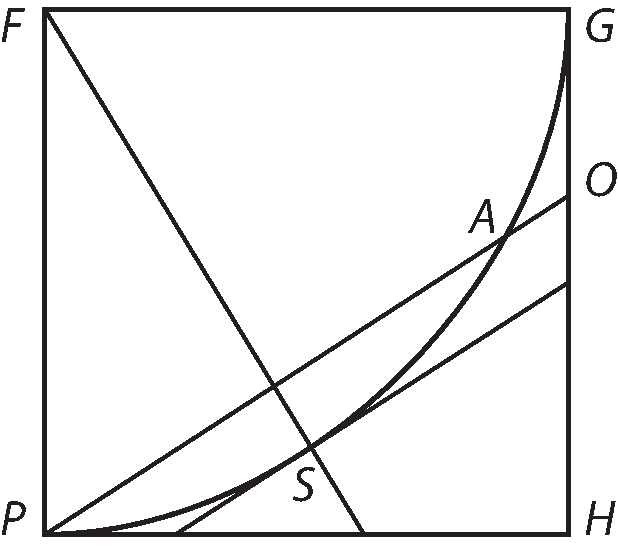
\includegraphics[trim = 0mm -3mm 0mm 0mm, clip, width=0.42\textwidth]{images/LH035,14,02_117r-d1.pdf}\\
%\noindent \centering [\textit{Fig. 1}]\edtext{}{\lemma{[\textit{Fig. 1}]}\killnumber\Cfootnote{\cite{00301}Vgl. a.a.O., Fig. 49 (\cite{01008}\textit{WO} I, S. 611).}}%
%\pend
%\vspace{2.0em}
%%%%%%%%%%%%%%%%%%%% 
\pstart
\begin{wrapfigure}[12]{l}{0.36\textwidth}
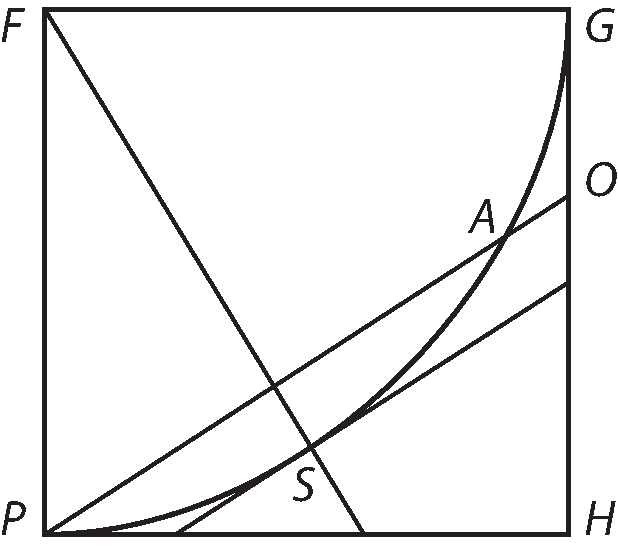
\includegraphics[trim = 0mm -3mm -5mm 0mm, clip, width=0.36\textwidth]{images/LH035,14,02_117r-d1.pdf}\\
\noindent \centering [\textit{Fig. 1}]\edtext{}{\lemma{\hspace{2mm}[\textit{Fig. 1}]}\killnumber\Cfootnote{\cite{00301}Vgl. a.a.O., Fig. 49 (\cite{01008}\textit{WO} I, S. 611).}} 
\end{wrapfigure}
Vera haec, sed nemo ex propositione sic divinaret,
crederet enim potius, quanto ictu impresso quousque elevari debeat.
Res ex ejus sensu tali exemplo declarari potest:
\edtext{si $\displaystyle P$ suspensum ex filo $\displaystyle FP$
sit pondus\protect\index{Sachverzeichnis}{pondus} compositum%
}{\lemma{si $\displaystyle P$}\Bfootnote{%
\textit{(1)}\ sit com
\textit{(2)}\ suspensum [...] compositum
\textit{L}}}
ex plumbo\protect\index{Sachverzeichnis}{plumbum}
et subere\protect\index{Sachverzeichnis}{suber},
plumbo intra lignum\protect\index{Sachverzeichnis}{lignum} abscondito,
pendulum\protect\index{Sachverzeichnis}{pendulum} ejusmodi
in aqua\protect\index{Sachverzeichnis}{aqua} locatum
ascendet ad certum usque inclinationis gradum,
si levitas\protect\index{Sachverzeichnis}{levitas} ligni sit
ad gravitatem\protect\index{Sachverzeichnis}{gravitas} plumbi, ut $\displaystyle OH$ ad $\displaystyle PH,$
ascendet perpendiculum\protect\index{Sachverzeichnis}{perpendiculum} usque in $\displaystyle S.$
Et ita jucundum exhibebitur spectaculum\protect\index{Sachverzeichnis}{spectaculum}
quo perpendiculum in media
\edtext{aqua stabit certa quadam ratione mirantibus spectatoribus inclinatum.%
}{\lemma{aqua}\Bfootnote{%
\textit{(1)}\ velut erectum stabit:
\textit{(2)}\ stabit [...] inclinatum.
\textit{L}}}
Quod si possit tegi filum\protect\index{Sachverzeichnis}{filum} suspendens
mirabitur spectator tanto magis.
Interea [indicis]\edtext{}{\lemma{indici}\Bfootnote{\textit{ändert Hrsg.}}}
digitis ostensio, et varia jam sic spectacula\protect\index{Sachverzeichnis}{spectaculum} exhiberi possunt.
(+~Eadem serviunt
\edtext{ad mirum librae\protect\index{Sachverzeichnis}{libra} genus.~[+)]}{\lemma{ad}\Bfootnote{%
\textit{(1)}\ pondus
\textit{(2)}\ mirum librae genus
\textit{L}}}
Sit perpendiculum\protect\index{Sachverzeichnis}{perpendiculum} ejusmodi
in aqua suspensum angulo si placet semirecto.
Inde assurgat aliquid recte, imponendi ponderis capax, extra aquam\protect\index{Sachverzeichnis}{aqua}.
Quod exit subtilissimum esse debet,
ne ponderis ejus ratio habeatur,
nisi malimus rem ponderandam[,]
cum est subtili inclusam vitreo globulo[,]\protect\index{Sachverzeichnis}{globulus vitreus}
in ipsa aqua ponderare.
Imo ne pondus\protect\index{Sachverzeichnis}{pondus} rei exeuntis quicquam faciat,
effici potest, ut quantum intrat, tantum exeat in circulum
aut ut in aequilibri balancier\protect\index{Sachverzeichnis}{balancier}.
Quo posito tantum objici potest aquae inaequalitas,
et praeterea calculo opus, ob actionem obliquam.
Melior ergo haud dubie altera erit libra,\protect\index{Sachverzeichnis}{libra}
solius penduli\protect\index{Sachverzeichnis}{pendulum} ope,
nunc tantum admoneam aliam applicationem hujus principii superesse perelegantem.
\edtext{Nimirum
%
[117~v\textsuperscript{o}] %%%%%%%%%%  HIER BEGINNT BLATT 117v.
%
concavitate inter}{\lemma{Nimirum}\Bfootnote{%
\textit{(1)}\ inter
\textit{(2)}\ concavitate inter
\textit{L}}}
duos globos\protect\index{Sachverzeichnis}{globus} relicta et liquore\protect\index{Sachverzeichnis}{liquor} repleta,
in quo globuli vitrei\protect\index{Sachverzeichnis}{globulus vitreus}
prout opus gravati non nisi ad certam altitudinem ascendere descendereve
\edtext{possunt. Opus est}{\lemma{possunt.}\Bfootnote{%
\textit{(1)}\ An
\textit{(2)}\ Opus est
\textit{L}}}
autem ut globuli illi\protect\index{Sachverzeichnis}{globulus vitreus} fere
utrobique tangant duas quibus intercipiuntur sphaeras,
ita tamen ut aliqua sit illis ascendendi descendendique libertas.
Hoc \edtext{modo concavitas}{\lemma{modo}\Bfootnote{%
\textit{(1)}\ globus
\textit{(2)}\ concavitas
\textit{L}}}
$\displaystyle EF$ quasi in zonas\protect\index{Sachverzeichnis}{zona} dividi pot-
\pend
\newpage
\pstart
\noindent 
\begin{window}[0,r,\hspace{4mm}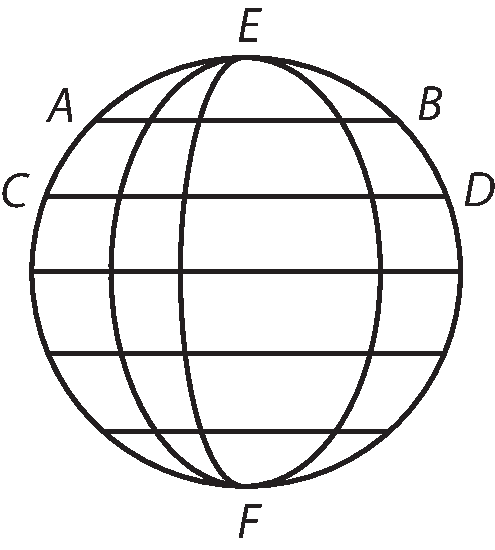
\includegraphics[%trim = -3mm -2mm 0mm 0mm, clip,
width=0.28\textwidth]
{images/LH035,14,02_117v-d1.pdf}, \centering{[\textit{Fig. 2}] \vspace{4mm}}]
\noindent
%\begin{wrapfigure}[10]{l}{0.28\textwidth} \noindent \vspace*{-1.5em}
%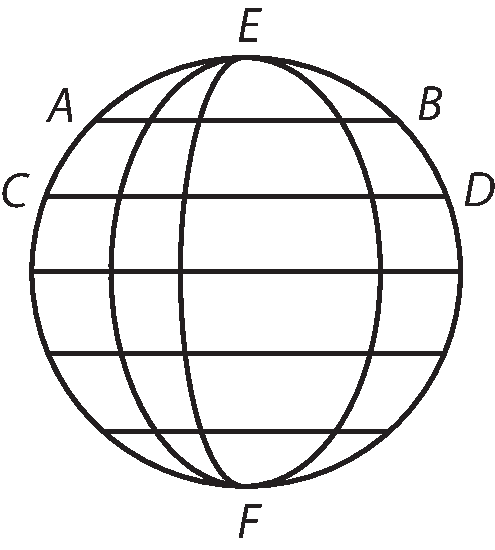
\includegraphics[trim = 0mm -1mm -5mm 0mm, clip, width=0.28\textwidth]{images/LH035,14,02_117v-d1.pdf}\\
%\noindent
%\centering
%[\textit{Fig. 2}]
%\end{wrapfigure}
est aut climata,\protect\index{Sachverzeichnis}{clima} in quibus morentur,
instar superficiei sphaerae terrestris.
Servit ad res in classes distinguendas,
ita tamen ut in singulis classibus divisione aut certa fixa sede opus non sit:
applicari potest ad Hierarchiam novem
\edtext{ordinibus angelorum\protect\index{Sachverzeichnis}{angelus}}{\lemma{\hspace*{1,8mm}4f. \hspace*{1,8mm}ordinibus}\killnumber\Bfootnote{%
\textit{(1)}\ angulorum
\textit{(2)}\ angelorum
\textit{L}}}
etc. et {daemonum\reversemarginpar\marginnote{\scriptsize\hspace{-13mm}5}},\protect\index{Sachverzeichnis}{daemon}
\edtext{Tabulam Zebetis,\protect\index{Namensregister}{\textso{Kebes} (Cebes, Zebes) von Theben, 5./4. Jh. v. Chr.}}{\lemma{\hspace*{1,8mm}5 \hspace*{1,8mm}Tabulam Zebetis}\killnumber\Cfootnote{\cite{01053} \textsc{Epiktet}, \textit{Enchiridion. Una cum Cebetis Thebani tabula}, Leiden und Antwerpen 1670. Siehe \cite{01054}\textit{LSB} VI, 3, N. 24.}}
animalia et habitus Europae,\protect\index{Ortsregister}{Europa}
Africae,\protect\index{Ortsregister}{Africa} Asiae\protect\index{Ortsregister}{Asia} etc.
prorsus ut pictura sit facta in globo.\protect\index{Sachverzeichnis}{globus}
Partiri \edtext{licebit in varios}{%
\lemma{\hspace*{1,8mm}7 \hspace*{1,8mm}licebit}\killnumber\Bfootnote{%
\textit{(1)}\ pro vari
\textit{(2)}\ in varios
\textit{L}}}
quasi meridianos,\protect\index{Sachverzeichnis}{meridianus}
qui liquoribus\protect\index{Sachverzeichnis}{liquor} aut saltem globis communicationem negent,
ita quaelibet cellula,\protect\index{Sachverzeichnis}{cellula}
vel interceptio meridianorum novum ordinis {genus\reversemarginpar\marginnote{\scriptsize\hspace{-13mm}10}} dabit.
%
[118~r\textsuperscript{o}]%%%%%%%%%%  HIER BEGINNT BLATT 118r (118v ist leer)
%
\end{window}
\pend
\count\Bfootins=1200
\count\Cfootins=1200
%\newpage
% PR: Abstand erforderlich. Breite des Abstands anpassungsfähig.
\pstart \vspace{0.3em} \protect\rule[-4mm]{0mm}{10mm}\setline{11}Wallis,\protect\index{Namensregister}{\textso{Wallis} (Wallisius), John 1616-1703} part. 1. cap. 3. prop. 24,
\edtext{aliquando ita accurate facta est libra
\textit{ut} $\displaystyle\frac{1}{400}$ma
\textit{grani huc illuc vertatur, imo}[,]
\textit{quod in honoratissimi Boylii\protect\index{Namensregister}{\textso{Boyle} (Boylius, Boyl), Robert 1627-1691} quadam bilance observatum est}[,]
\textit{parte unius grani \protect\rule[-4mm]{0mm}{10mm}$\displaystyle\frac{1}{1024}$.
quod coram compluribus testibus fide dignis experimento facto
saepius comprobatum fuit.}%
}{\lemma{aliquando [...] \textit{fuit}}\Cfootnote{\cite{00301}J. \textsc{Wallis}, \textit{Mechanica}, pars I, cap. 3, London 1670-1671, S. 108 (\cite{01008}\textit{WO} I, S. 641). Zitat mit Auslassungen.}}
\pend
\pstart%
%$\displaystyle \frac{1}{\infty}$ pars infinitesima.
\protect\rule[-4mm]{0mm}{10mm}\edtext{$\displaystyle \frac{1}{\infty}$ pars infinitesima.}
{\lemma{$\displaystyle \frac{1}{\infty}$ pars infinitesima.}\Cfootnote{\cite{00301}J. \textsc{Wallis}, \textit{Mechanica}, pars II, cap. 4, London 1670-1671, S. 110 (\cite{01008}\textit{WO} I, S. 645)}}
\quad
$\displaystyle \frac{\phantom{++}}{\phantom{++}}$
\quad
$\displaystyle \efrac{\vphantom{+}}{\displaystyle\efrac{\displaystyle +}{\displaystyle\efrac{\displaystyle -}{}}}a \efrac{\vphantom{+}}{\displaystyle\efrac{\displaystyle -}{\displaystyle\efrac{\displaystyle +}{}}}b$ est eorum differentia.
\pend
\vspace{0.3em}% PR: Abstand erforderlich. Breite des Abstands anpassungsfähig.
\pstart
Cap. V est instar
\edtext{libri, est de}{\lemma{libri,}\Bfootnote{%
\textit{(1)}\ de
\textit{(2)}\ est de
\textit{L}}}
calculo centri gravitatis\protect\index{Sachverzeichnis}{centrum gravitatis}.
Repetit quaedam ex sua \edtext{\textit{arith\-metica infinitorum}}{%
\lemma{\textit{arithmetica infinitorum}}%
\Cfootnote{J.\cite{00315} \textsc{Wallis}, \textit{Arithmetica infinitorum, seu Nova methodus inquirendi in curvilineorum quadratura}, Oxford 1656.}}\edtext{.\\%
\hspace*{7,5mm}%
Cap. 5. prop. 1. \textit{Si}}{\lemma{\textit{infinitorum.}}\Bfootnote{%
\textit{(1)}\ \textit{Si}
\textit{(2)}\ Cap. [...] \textit{Si}
\textit{L}}}%
\edtext{\textit{ intelligatur infinita series quantorum ab ipso capite seriei}[,]
\textit{puta $\displaystyle 0$ vel \protect\rule[-4mm]{0mm}{10mm}$\displaystyle\frac{1}{0}$}[,]
\textit{inchoatorum, et continue crescentium secundum seriem primanorum}[,]
\textit{secundanorum, etc.}
vel \textit{subsecundanorum}[,]
\textit{subtertianorum etc. eorumve reciprocam,}
[\textit{quorum}]\edtext{}{\lemma{quarum}\Bfootnote{\textit{L ändert Hrsg. nach Vorlage}}}
\textit{ultimum datum sit;
erit totius ratio ad seriem totidem ultimo aequalium,
ea quae est unius ad indicem seriei uno auctum.}
Ita seriei secundanorum index 2
\edtext{erit trilineum parabolicum}{\lemma{erit}\Bfootnote{%
\textit{(1)}\ parabola
\textit{(2)}\ complementum
\textit{(3)}\ trilineum parabolicum
\textit{L}}}
ad \edtext{rectangulum isoparallelum,}{\lemma{rectangulum}\Bfootnote{%
\textit{(1)}\ circumscriptum
\textit{(2)}\ isoparallelum
\textit{L}}}
ut 1 ad $\displaystyle\efrac{}{\displaystyle\efrac{\underbrace{2+1}}{3}}.$
% ERSETZT: $\displaystyle\begin{array}{cc} \underbrace{2+1} \\ 3 \end{array}.$
Ita in subsecundanis
[quorum]\edtext{}{\lemma{quarum}\Bfootnote{\textit{L ändert Hrsg.}}}
index $\displaystyle\frac{1}{2},$
erit parabola ad
\edtext{Rectang. isoparallelum,}{\lemma{Rectang.}\Bfootnote{%
\textit{(1)}\ circumscriptum
\textit{(2)}\ isoparallelum
\textit{L}}}
\protect\rule[-4mm]{0mm}{10mm}ut 1 ad $\displaystyle 1 + \frac{1}{2}$
seu ut 1 ad $\displaystyle\frac{3}{2}$
seu ut 2 ad 3.%
}{\lemma{\textit{Si intelligatur} [...] 2 ad 3}\Cfootnote{J.\cite{00301} \textsc{Wallis}, \textit{Mechanica}, pars II, cap. 5, London 1670-1671, S. 148 (\cite{01008}\textit{WO} I, S. 667f.). Zitat mit Auslassungen.}}
\pend
\count\Bfootins=1500
\count\Cfootins=1500
\pstart
Ut autem intelligatur quid sit index[,] sciendum idem esse quod
\edtext{exponentem abscissae,}{\lemma{}\Bfootnote{exponentem\ \textbar\ incognitae seu \textit{gestr.}\ \textbar\ abscissae \textit{L}}}
quae explicat valorem ordinatae,
v.g. $\displaystyle\sqrt{\vphantom{\Large{hy}}}$\!{\textcircled{$\scriptstyle 3$}}$\displaystyle x^4 \sqcap\, y.$
erit index seu exponens seriei: $\displaystyle 4 \smallsmile 3.$
Nempe extractio divisione,
in se ductio multiplicatione,
divisio substractione repraesentatur[;]
unde Reciprocorum iidem mole exponentes
qui directorum, sed negati,
v.g. \protect\rule[-4mm]{0mm}{10mm}$\displaystyle y^2 \sqcap\, x.$
est exponens $\displaystyle 2.$\quad%
$\displaystyle \sqrt{\vphantom{y}}y\, \sqcap\, x.$
est exponens $\displaystyle\frac{1}{2}.$\quad%
$\displaystyle\frac{1}{y^2} \sqcap\, x.$
est exponens $\displaystyle -2.$\quad%
et $\displaystyle\frac{1}{\sqrt{\vphantom{y}}y}\, [\sqcap\ x]$\edtext{}{\lemma{}\Bfootnote{$\displaystyle\sqcap\ x$\ \ \textit{erg. Hrsg.}\hspace{-3mm}}}
est exponens \protect\rule[-4mm]{0mm}{10mm}$\displaystyle -\frac{1}{2}.$
\pend
\pstart
Unde sequitur res in reciprocis satis notabilis.
Nempe ut ait Wallis\protect\index{Namensregister}{\textso{Wallis} (Wallisius), John 1616-1703}
\edtext{prop. 7.
\textit{Si intelligatur ex rectis planisve secundum aliquam ex
\edtext{reciprocis (\hspace{-1.2mm}\phantom)indicem}{\lemma{}\Bfootnote{\textit{reciprocis}\ \textbar\ \textit{in def. 2. gestr.}\ \textbar\ \textit{(\hspace{-1.2mm}\phantom)indicem} \textit{L}\hspace{-3mm}}}
habentibus negativum) seriem infinitam,
(ab \protect\rule[-4mm]{0mm}{10mm}$\displaystyle\frac{1}{0}$ ipsa seriei origine inchoatam,
et dato terminatam) figura conflari:
Habebit haec ad verticem latitudinem infinitam,
finitam tamen, si ex parte verticis intelligatur vel tantillum plano parallelo abscindi
(adeoque figura saltem truncata magnitudinis erit finitae:}[\textit{)}]\edtext{}{\lemma{}\Bfootnote{\textit{)\ \ erg. Hrsg.}}}
\textit{Aream vero quae sit ad parallelogrammum vel solidum prismaticum
super aequali basi aeque altum, ut $\displaystyle 1$ ad indicem unitate auctum,
adeoque vel magnitudine finitam si index sit major quam \protect\rule[-4mm]{0mm}{10mm}$\displaystyle -1$}[,]
\textit{puta $\displaystyle -\frac{1}{4}.$ $\displaystyle -\frac{1}{2}.$
\edtext{$\displaystyle -\frac{1}{3}.$}{%
\lemma{$\displaystyle -\frac{1}{3}$}%
\Cfootnote{In der Vorlage $\displaystyle -\frac{3}{4}.$}}
vel infinitam si index sit $\displaystyle -1$}
(+~ut in Hyperbola Apolloniana~+)
\textit{vel plusquam infinitam,
si sit index minor
\edtext{quam $\displaystyle -1.$}{\lemma{}\Bfootnote{\textit{quam}\ \textbar\ plusquam \textit{gestr.}\ \textbar\ $\displaystyle -1.$\ \textit{L}}}
puta $\displaystyle -2.$ $\displaystyle -3$ etc.}%
}{\lemma{prop. 7. [...] \textit{etc.}}\Cfootnote{\cite{00301}a.a.O., S. 165 (\cite{01008}\textit{WO} I, S. 679). Zitat mit Auslassung.}}
\pend
\pstart
% \vspace*{1.0em}% PR: Rein provisorisch !!!
\noindent
\centering
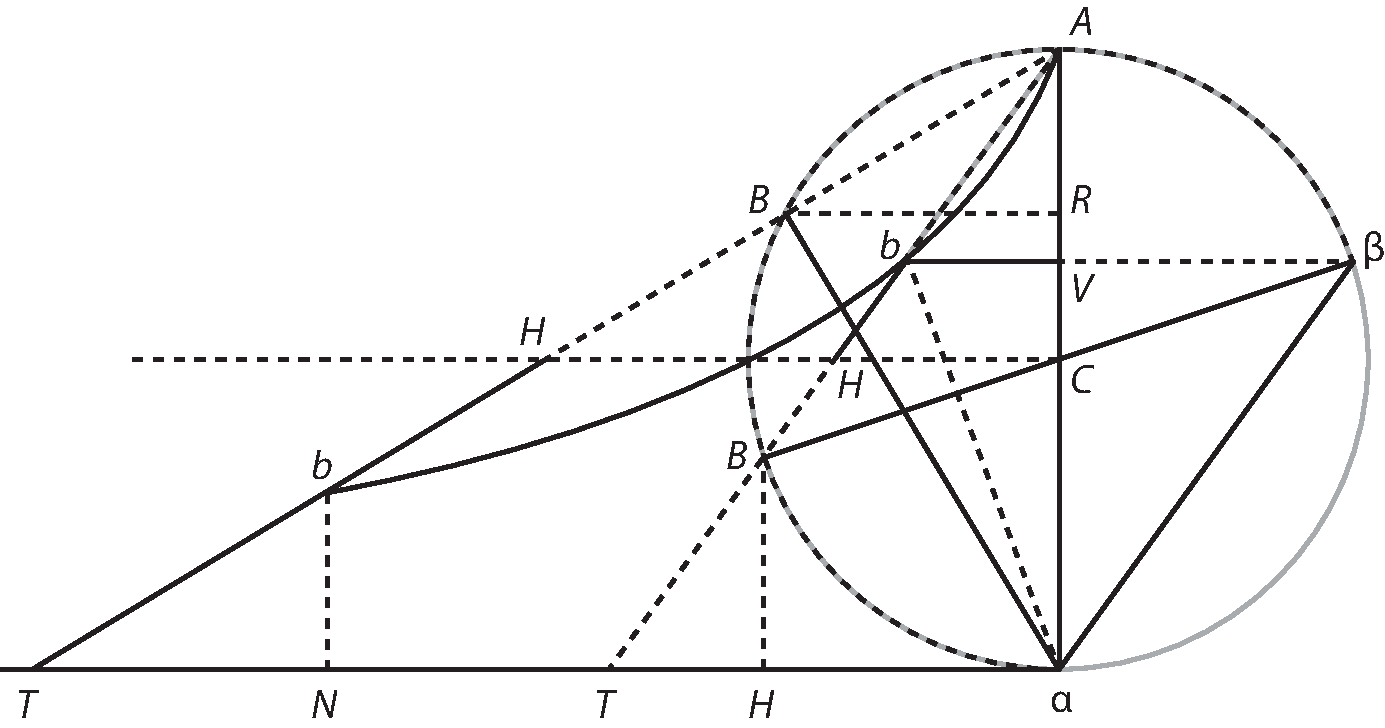
\includegraphics[trim = 0mm -3mm 0mm 0mm, clip, width=0.9\textwidth]{images/LH035,14,02_118r-d1.pdf}\\
\noindent \centering [\textit{Fig. 3, tlw. Blindzeichnung}]\edtext{}{\lemma{\hspace*{1,8mm}[\textit{Fig. 3}]}\killnumber\Cfootnote{\cite{00301}Vgl. a.a.O., Fig. 205 (\cite{01008}\textit{WO} I, S. 904).}}%
\pend
\count\Bfootins=1200
\count\Cfootins=1200
\vspace{1em}
\pstart
\advanceline{-2}
\edtext{%
De cissoeide haec habet Wallisius\protect\index{Namensregister}{\textso{Wallis} (Wallisius), John 1616-1703}
Cap. V. prop. 29 \edtext{et in part. 3. Epilogo ex Miscellaneis prop. 2}{\lemma{et in [...] prop. 2}\Bfootnote{\textit{erg. L}}}.%
}{\lemma{De cissoeide [...] prop. 2}\Cfootnote{\cite{00301}a.a.O., S. 531-533 und pars III, cap. 15, S. 754-759 (\cite{01008}\textit{WO} I, S. 904-910).}}
\edtext{%
\textit{Cissoeidis lineae meminit Pappus\protect\index{Namensregister}{\textso{Pappos} (Pappus) von Alexandrien, um 300}
lib. 3, prop. 5 pro duabus mediis proportionalibus inveniendis excogitatae.
Cujus haec natura},
ut \edtext{$\displaystyle ABB\alpha$ semicirculus}{%
\lemma{$\displaystyle ABB\alpha$}\Bfootnote{%
\textit{(1)}\ arcus circuli
\textit{(2)}\ semicirculus
\textit{L}}}
centro $\displaystyle C.$
angulus $\displaystyle HCA$ rectus.
$\displaystyle HB\, \sqcap\, Hb.$
cissoeides $\displaystyle Abb.$%
}{\lemma{\textit{Cissoeidis} [...] $\displaystyle Abb$}\Cfootnote{\cite{00301}a.a.O., pars II, cap. 5, S. 531 (\cite{01008}\textit{WO} I, S. 904). Vgl. \textsc{Pappos}, \textit{Mathematica collectio}, l. III, probl. I, prop. V.\cite{01015}}}
\edtext{%
Aliter construi potest eadem curva ex Pappo.\protect\index{Namensregister}{\textso{Pappos} (Pappus) von Alexandrien, um 300}
Nempe ipsis sinui recto \edtext{$\displaystyle V\beta$}{\lemma{$\displaystyle V\beta$}\Bfootnote{\textit{erg. L}}}
et verso \edtext{$\displaystyle AV$}{\lemma{$\displaystyle AV$}\Bfootnote{\textit{erg. L}}}
tertia proportionalis est applicata ex curva ad axem seu diametrum circuli, $\displaystyle bV.$
Nempe ducta diametro $\displaystyle BC\beta$
et junctis $\displaystyle A\beta,$ $\displaystyle bV\beta.$
patet in $\displaystyle\largetriangledown$\textsuperscript{lo} $\displaystyle \beta bB,$
ob $\displaystyle bB$ et $\displaystyle B\beta$ bisectas recta $\displaystyle HC.$
esse $\displaystyle HC,$ et $\displaystyle bV\beta$ parallelas.
Ergo anguli ad $\displaystyle V$ recti.
Ergo $\displaystyle V\alpha,$ $\displaystyle V\beta,$ $\displaystyle VA,$ $\displaystyle Vb$ continue proportionales.
Ergo positis $\displaystyle AV\, \sqcap\, v$
et $\displaystyle V\beta\, \sqcap\, s$
(sinu verso et recto)
\protect\rule[-4mm]{0mm}{10mm}erit: $\displaystyle Vb\, \sqcap \frac{v^2}{s}$
seu $\displaystyle\sqcap\ \protect\frac{v^2}{\sqrt{2av - v^2}}.$%
}{\lemma{Aliter [...] $\displaystyle \protect\frac{v^2}{\sqrt{2av - v^2}}$}\Cfootnote{\cite{00301}\textsc{J. Wallis}, \textit{Mechanica}, pars II, cap. 5, London 1670-1671, S. 533 (\cite{01008}\textit{WO} I, S. 905). Vgl. \textsc{Pappos}, \textit{Mathematica collectio}, l. III, probl. I, prop. V.\cite{01015}}}%
\edlabel{LH035,14,02_118r_01}\edtext{}{{\xxref{LH035,14,02_118r_01}{LH035,14,02_118r_02}}\lemma{$\displaystyle \protect\frac{v^2}{\sqrt{2av - v^2}}.$}\Bfootnote{%
\textit{(1)}\ Porro ut primus notavit Hugenius\protect\index{Namensregister}{\textso{Huygens} (Hugenius, Ugenius, Hugens, Huguens), Christiaan 1629-1695}
portiones $\displaystyle b\alpha A,$ aequales
\textit{(2)}\ Est [...] notabilis
\textit{L}}}
\pend
\count\Bfootins=900
\count\Cfootins=900
\pstart
Est et alia hujus curvae proprietas notabilis.\edlabel{LH035,14,02_118r_02}
\edtext{%
Producatur $\displaystyle Ab.$
Dum occurrat tangenti oppositi circuli verticis $\displaystyle \alpha,$
nempe ipsi $\displaystyle \alpha T,$
in punctis $\displaystyle T$
erit ubiqe \edtext{$\displaystyle \alpha T\, \sqcap\, b\beta$ quia}{%
\lemma{$\displaystyle \sqcap\, b\beta$}\Bfootnote{%
\textit{(1)}\ seu e
\textit{(2)}\ quia
\textit{L}}}
$\displaystyle AT$ et $\displaystyle \beta\alpha$ parallelae,%
}{\lemma{Producatur [...] parallelae}\Cfootnote{\cite{00301}\textsc{J. Wallis}, \textit{Mechanica}, pars III, cap. 15, London 1670-1671, S. 754 (\cite{01008}\textit{WO} I, S. 906).}}
quod probo,
quia idem angulus $\displaystyle AB\beta,$ et $\displaystyle B\beta\alpha$
ad eandem rectam $\displaystyle B\beta.$
Nam arcus $\displaystyle \alpha B$ $\displaystyle \sqcap$
\edtext{arcui}{\lemma{arcui}\Bfootnote{\textit{erg. L}}}
\edtext{$\displaystyle A\beta.$
Est et alia proprietas, quod semper}{%
\lemma{$\displaystyle A\beta.$}\Bfootnote{%
\textit{(1)}\ Unde et semper
\textit{(2)}\ Est [...] semper
\textit{L}}}
$\displaystyle AB\, \sqcap\, bT$
vel $\displaystyle BT\, \sqcap\, Ab,$
quia $\displaystyle H\alpha\, \sqcap\, V\beta.$
ergo $\displaystyle bV\, \sqcap\, TH.$
ergo $\displaystyle BH\, \sqcap\, AV,$
vel $\displaystyle BT\, \sqcap\, Ab.$
vel denique $\displaystyle bT\, \sqcap\, AB.$
quod ex eo potuisset probari,
quia $\displaystyle AH\, \sqcap\, HT.$
Jam \edtext{%
Hugenius\protect\index{Namensregister}{\textso{Huygens} (Hugenius, Ugenius, Hugens, Huguens), Christiaan 1629-1695}
observat spatium $\displaystyle AbbT\alpha\ \sqcap$
triplo segmento $\displaystyle BB\alpha B$
addito $\displaystyle\largetriangledown$\textsuperscript{lo} $\displaystyle AB\alpha.$%
}{\lemma{Hugenius [...] $\displaystyle\largetriangledown$\textsuperscript{lo} $\displaystyle AB\alpha$}%
\Cfootnote{\cite{00301}a.a.O., S. 754 (\cite{01008}\textit{WO} I, S. 906f.).
Siehe C.\cite{01068} \textsc{Huygens}, \textit{Brief an J. Wallis vom April 1658}, in \textit{HO} II, S. 170-173.}}
\edtext{%
Wallisius\protect\index{Namensregister}{\textso{Wallis} (Wallisius), John 1616-1703} sic enuntiat brevius:
spatium $\displaystyle Abb\alpha\ \sqcap$
triplo segmento $\displaystyle BB\alpha B.$%
}{\lemma{Wallisius [...] $\displaystyle BB\alpha B$}\Cfootnote{J.\cite{00301} \textsc{Wallis}, \textit{Mechanica}, p. III, c. 15, London 1670-1671, S. 758 (\cite{01008}\textit{WO} I, S. 909f.).}}\edtext{
Cum sit $\displaystyle AB\, \sqcap\, bT.$
erit $\displaystyle bN\, \sqcap\, AV.$}{\lemma{%
$\displaystyle BB\alpha B.$}\Bfootnote{%
\textit{(1)}\ Nota est $\displaystyle \alpha b\, \sqcap\, \alpha B.$ NB.
\textit{(2)}\ Cum [...] $\displaystyle AV$
\textit{L}}}
%
[119~r\textsuperscript{o}] %%%%%%%%%%  HIER BEGINNT BLATT 119r (118v ist leer).
%
\pend
\vspace*{1.0em}% PR: Abstand erforderlich. Breite des Abstands anpassungsfähig.
\pstart
\noindent
\edtext{%
Wallisii\protect\index{Namensregister}{\textso{Wallis} (Wallisius), John 1616-1703}
\textit{Mechanica de Motu}\cite{00301} pars III\textsuperscript{tia}
ubi de vecte\protect\index{Sachverzeichnis}{vectis}
et reliquis illis machinis quas vocant fundamentales\protect\index{Sachverzeichnis}{machina fundamentalis}
et \textit{Motibus compositis\protect\index{Sachverzeichnis}{motus compositus}
acceleratis\protect\index{Sachverzeichnis}{motus acceleratus},
retardatis\protect\index{Sachverzeichnis}{motus retardatus},
et projectorum\protect\index{Sachverzeichnis}{motus projectorum};
de percussione\protect\index{Sachverzeichnis}{percussio},
de cuneo\protect\index{Sachverzeichnis}{cuneus},
de Elatere\protect\index{Sachverzeichnis}{elater},
et Resilitione\protect\index{Sachverzeichnis}{resilitio}
seu Reflexione\protect\index{Sachverzeichnis}{reflexio},
de Hydrostaticis\protect\index{Sachverzeichnis}{hydrostatica}
et aeris aequipondio\protect\index{Sachverzeichnis}{aequipondium aeris}
deque variis quaestionibus Mechanicis.}\protect\index{Sachverzeichnis}{quaestio mechanica}}{%
\lemma{Wallisii [...] \textit{Mechanicis}}%
\Cfootnote{Nach J.\cite{00301} \textsc{Wallis}, \textit{Mechanica}, London 1670-1671, Titelblatt des dritten Teils.}}
Mihi unica pars 3\textsuperscript{tia}
\edtext{videtur vere Mechanica%
}{\lemma{videtur}\Bfootnote{%
\textit{(1)}\ utilis illis qui
\textit{(2)}\ vere Mechanica
\textit{L}}}%
\edtext{, nam%
}{\lemma{Mechanica}\Bfootnote{%
\textit{(1)}\ reliqua enim
\textit{(2)}\ nam
\textit{L}}}
parte \edtext{prima generalia,%
}{\lemma{prima}\Bfootnote{%
\textit{(1)}\ non
\textit{(2)}\ generalia
\textit{L}}}
parte 2\textsuperscript{da}, vix nisi Geometrica habentur.
\pend
\vspace*{1.0em}
\pstart 
\textso{Cap. 6. prop. 1.}
ubi de vecte.
\edtext{\textit{Sic aliquando} in \textit{plura distribuitur motus,
ut} ambiguum \textit{sit,}
\edtext{quid sit \textit{fulcrum},\protect\index{Sachverzeichnis}{fulcrum}
quid \textit{mobile.}\protect\index{Sachverzeichnis}{mobile}%
}{\lemma{quid sit}\Bfootnote{%
\textit{(1)}\ vectis quid \textit{mobile}
\textit{(2)}\ \textit{fulcrum}, quid \textit{mobile}
\textit{L}}}
\textit{Sic \edtext{in navium%
}{\lemma{in}\Bfootnote{%
\textit{(1)}\ navis
\textit{(2)}\ \textit{navium}
\textit{L}}}
remis dum vis\protect\index{Sachverzeichnis}{vis} manubrio applicatur,
palmula aquae ut fulcro innixa scalmum cum conjuncta navi submovet.
Verum cum} non \textit{ita firmum fulcrum sit aqua, quin et ipsa nonnihil pressa cedat,
ratione motus hujus scalmus pro fulcro erit, aqua pro mobili.
Cum} vero et \textit{remus incurvetur;
hinc tertius oritur motus,}
et hi \textit{tres motus se minuunt invicem.}%
}{\lemma{\textit{Sic} [...] \textit{invicem}}\Cfootnote{\cite{00301}a.a.O., cap. 6, S. 575 (\cite{01008}\textit{WO} I, S. 943). Zitat mit Auslassungen.}}
\pend
\pstart
\edtext{Si ejusdem vectis duo fulcra $\displaystyle AC.$ $\displaystyle BD,$
obliquo situ non partiuntur onus aequaliter sed plus sustinet $\displaystyle AC$ inferior,
quod patet erigendo longam scalam aut perticam.
Nam si $\displaystyle AB$ plane fiat perpendicularis horizonti
$\displaystyle BD$ nihil feret, $\displaystyle AC$ omnia.
Hinc partiri \edtext{licebit onus%
}{\lemma{licebit}\Bfootnote{%
\textit{(1)}\ vires
\textit{(2)}\ onus
\textit{L}}}
in data ratione ipsa obliquitate.}{%
\lemma{Si ejusdem [...] obliquitate}%
\Cfootnote{\cite{00301}a.a.O., S. 581 (\cite{01008}\textit{WO} I, S. 947).}}
\pend
\count\Bfootins=1500
\count\Cfootins=1500
\pstart
\noindent
\begin{minipage}[c]{0.35\textwidth}
\centering
\hspace*{-5mm}
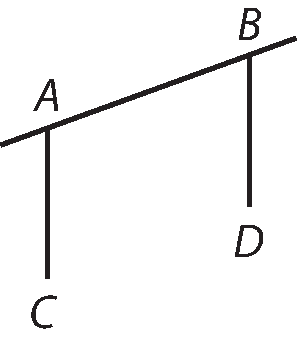
\includegraphics[width=0.55\textwidth]{images/LH035,14,02_119r-d1.pdf}%\\
\end{minipage}
%\hspace*{13mm}
%\vspace{-5mm}
\begin{minipage}[c]{0.65\textwidth}
\centering
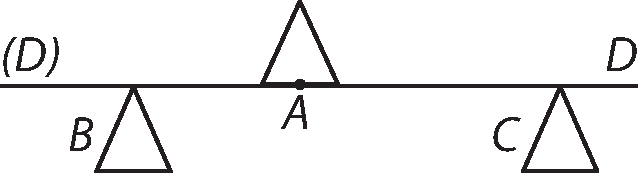
\includegraphics[width=0.6\textwidth]{images/LH035,14,02_119r-d2.pdf}%\\
\end{minipage}\\
\\
\vspace{1.5em}
\hspace*{13mm} [\textit{Fig. 4}]\hspace*{53mm} [\textit{Fig. 5, gestr.}]
\pend
\count\Bfootins=1500
\count\Cfootins=1500
\vspace*{3.0em}% PR: Rein provisorisch !!!
\pstart
\noindent
\advanceline{-2}[\textit{Folgender kleingedruckter Text gestrichen:}]
\pend
\vspace*{0.5em}
\pstart
\footnotesize
\edlabel{LH035,14,02_119r_01}\edtext{}{{\xxref{LH035,14,02_119r_01}{LH035,14,02_119r_02}}%
\lemma{}\Bfootnote{%
\textit{(1)}\ Quin etsi vectes
\textit{(2)}\ Prop. 5. 6. Vectis
\textit{L}}}%
\edtext{Prop. 5. 6. Vectis\protect\index{Sachverzeichnis}{vectis}%
\edlabel{LH035,14,02_119r_02}
sit \edtext{horizontalis, pondere\protect\index{Sachverzeichnis}{pondus} suo onerans%
}{\lemma{horizontalis,}\Bfootnote{%
\textit{(1)}\ non sit sermo de ejus pondere, sed imposito tantum $\displaystyle A$
\textit{(2)}\ pondere suo onerans
\textit{L}}}
duo fulcra\protect\index{Sachverzeichnis}{fulcrum} $\displaystyle B.$ $\displaystyle C,$
tunc onus\protect\index{Sachverzeichnis}{onus} inter se partiuntur,
idque in ea ratione quae est reciproca distantiarum suarum a centro
\edtext{gravitatis\protect\index{Sachverzeichnis}{centrum gravitatis} $\displaystyle A.$ Itaque%
}{\lemma{}\Bfootnote{gravitatis\ \textbar\ vectis \textit{gestr.}\ \textbar\ $\displaystyle A.$ Itaque\ \textit{L}}}
magis premitur fulcrum, cui propius centrum gravitatis.
Nimirum ponatur vectis\protect\index{Sachverzeichnis}{vectis}
pondus\protect\index{Sachverzeichnis}{pondus} in punctum $\displaystyle A$ colligi.
Premitur fulcrum $\displaystyle B,$ tanta vi
quanta esset vis sustentatrix\protect\index{Sachverzeichnis}{vis sustentatrix} ponderis $\displaystyle A$
si abesset fulcrum\protect\index{Sachverzeichnis}{fulcrum} $\displaystyle B.$
Quod si jam abesset
\edtext{fulcrum $\displaystyle B,$ ponamus vim sustentatricem ponderis $\displaystyle A,$%
}{\lemma{fulcrum $\displaystyle B,$}\Bfootnote{%
\textit{(1)}\ tunc vi utique qua
\textit{(2)}\ ponamus [...] ponderis $\displaystyle A,$
\textit{L}}}
esse in puncto $\displaystyle D$ distantia qualibet $\displaystyle CD.$
Ut ergo sustineat, erit $\displaystyle D$ ad
\edtext{vim quam exercet}{\lemma{vim quam exercet}\Bfootnote{\textit{erg. L}}}
$\displaystyle A,$ ut $\displaystyle AC$ ad $\displaystyle DC$ seu in reciproca distantiarum.%
}{\lemma{Prop. 5. [...] distantiarum}\Cfootnote{a.a.O.,
S. 579-581 (\cite{01008}\textit{WO} I, S. 946f.).}}
\pend
\vspace{1.0em} 
\pstart
Cap. VI. \edtext{prop. 5.
\textit{Si vectis,\protect\index{Sachverzeichnis}{vectis}
(Tignum, palanga, Trabs oblonga)
situ horizontali jacens,
utroque sui extremo fulcris\protect\index{Sachverzeichnis}{fulcrum} sustineatur,
fulcra bina sustinentia onus\protect\index{Sachverzeichnis}{onus} inter se partiuntur,
idque in ea ratione, quae est reciproca distantiarum suarum
a vectis centro gravitatis,\protect\index{Sachverzeichnis}{centrum gravitatis}
et quidem utrumvis eam totius portionem sustinet,
quae ad totum eam habeat rationem,
quam habet contrarii fulcri distantia ad distantiam totam seu vectis longitudinem.}
Aequaliter partiuntur si centrum gravitatis sit in medio,
si non sit, id \textit{magis premitur cui propius centrum.}
Idem est si vectis\protect\index{Sachverzeichnis}{vectis} nullum intelligatur pondus,
sed is alio pondere\protect\index{Sachverzeichnis}{pondus}
\edtext{oneratus, quod censendum est
locatum, ubi est ejus centrum gravitatis.\protect\index{Sachverzeichnis}{centrum gravitatis}%
}{\lemma{oneratus,}\Bfootnote{%
\textit{(1)}\ cujus cent
\textit{(2)}\ quod [...] gravitatis.
\textit{L}}}%
}{\lemma{prop. 5. [...] gravitatis}\Cfootnote{\cite{00301}\cite{01008}a.a.O., S. 579f. (\textit{WO} I, S. 946).}}
\pend
\newpage
\count\Bfootins=1000
\count\Cfootins=1000
\pstart
\begin{wrapfigure}{l}{0.36\textwidth}
\vspace{-4mm}
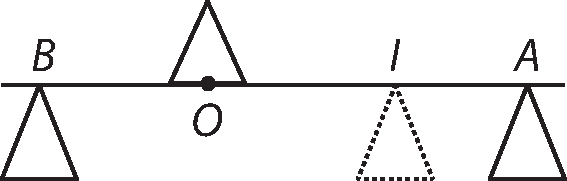
\includegraphics[trim = 0mm -3mm -5mm 0mm, clip, width=0.36\textwidth]{images/LH035,14,02_119r-d3.pdf}\\
% \vspace*{0,5mm}
\noindent
\centering
[\textit{Fig. 6}]\edtext{}{\lemma{\hspace*{1,8mm}[\textit{Fig. 6}]}\killnumber\Cfootnote{\cite{00301}Vgl. a.a.O., Fig. 232 (\cite{01008}\textit{WO} I, S. 947).}}%
\end{wrapfigure}
\edtext{$\displaystyle O$ centrum gravitatis,\protect\index{Sachverzeichnis}{centrum gravitatis}
fulcra\protect\index{Sachverzeichnis}{fulcrum} $\displaystyle B.$ $\displaystyle A.$
Tanto onere\protect\index{Sachverzeichnis}{onus} premitur fulcrum $\displaystyle A,$
quanto opus esset
\edtext{in $\displaystyle A$}{\lemma{in $\displaystyle A$}\Bfootnote{\textit{erg. L}}}
ad sustinendum pondus\protect\index{Sachverzeichnis}{pondus} $\displaystyle O$ si abesset $\displaystyle A.$
Porro minore opus est vi\protect\index{Sachverzeichnis}{vis sustentatrix}
ad sustinendum pondus $\displaystyle O$ in $\displaystyle A,$
quam ad sustinendum ipsum in $\displaystyle O.$
Sit vis in $\displaystyle A$ fulcro sustinens
ad vim ipsi $\displaystyle O$ aequalem seu in $\displaystyle O$ sustinentem, 
seu ad onus ut in reciproca ratione
\edtext{distantiarum, fulcri\protect\index{Sachverzeichnis}{fulcrum} et oneris,\protect\index{Sachverzeichnis}{onus}
seu ut}{\lemma{distantiarum,}\Bfootnote{%
\textit{(1)}\ seu ut
\textit{(2)}\ fulcri et oneris, seu ut
\textit{L}}}
$\displaystyle BO$ ad $\displaystyle BA.$
Ergo vis in $\displaystyle\protect\rule[-4mm]{0mm}{10mm} A\, \sqcap \frac{O \smallfrown BO}{BA}.$
Eodem modo vis in $\displaystyle B\, \sqcap \frac{O \smallfrown AO}{BA}.$
Ergo $\displaystyle\protect\rule[-4mm]{0mm}{10mm}\frac{\text{vis in } A}{\text{vis in } B} \sqcap \frac{BO}{AO}$ 
seu in reciproca distantiarum.%
}{\lemma{$\displaystyle O$ centrum [...] distantiarum}\Cfootnote{\cite{00301}a.a.O., S. 580f. (\cite{01008}\textit{WO} I, S. 946f.).}}
Perelegans demonstratio.
Hinc potest ita aptari locus ponderis,\protect\index{Sachverzeichnis}{pondus}
ut uno fulcro\protect\index{Sachverzeichnis}{fulcrum} existente altero
\edtext{debiliore, proportionaliter%
}{\lemma{debiliore,}\Bfootnote{%
\textit{(1)}\ nihilominus aequi
\textit{(2)}\ proportionaliter
\textit{L}}}
onerentur omnes.
Vellem tamen rigorosius ista demonstrari.
Nam supponitur ita inter calculum\protect\index{Sachverzeichnis}{calculus} unum omnia,
id scilicet quod subtrahi fingitur,
alterum nihil \edtext{substinere.\\%
\hspace*{7,5mm}Hinc%
}{\lemma{substinere.}\Bfootnote{%
\textit{(1)}\ An forte ita procedendum esset
\textit{(2)}\ Hinc
\textit{L}}}
jam \edtext{prop. 7 infert Wallisius,\protect\index{Namensregister}{\textso{Wallis} (Wallisius), John 1616-1703}
hinc calculari posse
\textit{quanta cuivis vectis\protect\index{Sachverzeichnis}{vectis} puncto firmitas requiratur ne}
\edtext{\textit{rumpatur}[,]
sive de solo vectis pondere,%
}{\lemma{\textit{rumpatur}}\Bfootnote{%
\textit{(1)}\ suo pondere.
\textit{(2)}\ sive de solo vectis pondere,
\textit{L}}}
sive et de alio imposito pondere\protect\index{Sachverzeichnis}{pondus}
quaestio \edtext{sit.
Nimirum}{\lemma{sit}\Bfootnote{%
\textit{(1)} , (nimirum
\textit{(a)}\ ponderum omnium onerantium
\textit{(b)}\ pondera omnium onerantia sive vectis solus, sive
\textit{(aa)}\ alia
\textit{(bb)}\ aliorum cum aut sine vecte pondus ponatur ex eorum centro gravitatis pendere. Inde
\textit{(2)} . Nimirum
\textit{L}}}
si de puncto aliquo quaeratur ut $\displaystyle I.$
tanta requiritur minimum firmitudo in $\displaystyle I.$
quanta opus esset fulcro in $\displaystyle I$ posito,
si nullo vinculo continerentur.
Quod fulcrum\protect\index{Sachverzeichnis}{fulcrum} imaginarium punctis repraesento,
erunt enim quasi duo vectes\protect\index{Sachverzeichnis}{vectis} $\displaystyle BI.$ $\displaystyle IA$
habentes unum fulcrum commune,
quod proinde centro gravitatis\protect\index{Sachverzeichnis}{centrum gravitatis}
tum ponderum omnium in $\displaystyle BI$
tum ponderum omnium in $\displaystyle IA,$
oneratum intelligendum est.%
}{\lemma{prop. 7 [...] intelligendum est}\Cfootnote{\cite{00301}a.a.O., S. 582f. (\cite{01008}\textit{WO} I, S. 948).}}
Mihi haec rationi satis consentanea videntur,
etsi nescio \edtext{quid contra margini ascripserit
Hugenius\protect\index{Namensregister}{\textso{Huygens} (Hugenius, Ugenius, Hugens, Huguens), Christiaan 1629-1695}
in suo Wallisii\protect\index{Namensregister}{\textso{Wallis} (Wallisius), John 1616-1703} exemplari.%
}{\lemma{quid [...] exemplari}\Cfootnote{Ein Exemplar der 1670/71-Ausgabe von Wallis' \textit{Mechanica} ist in dem Katalog verzeichnet, der kurz nach Huygens' Tode 1695 für die öffentliche Auktion seiner Buchsammlung erstellt wurde: Siehe \cite{01090}\textit{Catalogus ... librorum, praecipue mathematicorum, politicorum et miscellaneorum ... Christiani Hugenii}, den Haag 1695, S. 8 (Libri mathematici in quarto, Nr. 104; der Katalog ist in \cite{00113}\textit{HO} XXII zwischen S. 816 und S. 817 abgedruckt). Dieses Exemplar der \textit{Mechanica} ist aller Wahrschein\-lichkeit nach dasjenige, das Leibniz zum Exzerpieren vorlag und in dem er Huygens' Randbemerkungen lesen konnte. Dessen Spuren lassen sich nach der genannten Auktion nicht weiter verfolgen.}}
Unum notandum, etsi hic dicatur fulcro hoc
quo ait Wallisius\protect\index{Namensregister}{\textso{Wallis} (Wallisius), John 1616-1703} modo onerari[,]
hoc tamen intelligendum est, si scilicet ambo
\edtext{sustineant.
Sed hoc videtur nihil esse.
Nam si%
}{\lemma{sustineant.}\Bfootnote{%
\textit{(1)}\ Nam si vel unum ex illis sit debilius, toto
\textit{(2)}\ Sed hoc [...] Nam si
\textit{L}}}
scilicet ponantur sustinere,
nihil amplius habemus quod quaeramus.
Quaeritur enim quanta vi opus sit, ut sustineant,
id est quae sit vis minima sustinens,\protect\index{Sachverzeichnis}{vis sustentatrix}
seu maxima non sustinens in fulcris.
Et sciendum proinde est,
cuilibet fulcro\protect\index{Sachverzeichnis}{fulcrum} totam vim sustinendam, saltem pro distantiae ratione variatam,
itaque non dicendum esse vim totam esse partitam.
Nam in pluribus ejusmodi concinnantibus nullus est locus
qui non sustineat totam massam\protect\index{Sachverzeichnis}{massa}\textso{ dis\-junctive,}
in eo igitur
%
[119~v\textsuperscript{o}] %%%%%%%%%%  HIER BEGINNT BLATT 119v.
%
hallucinatus videtur Wallisius\protect\index{Namensregister}{\textso{Wallis} (Wallisius), John 1616-1703}
qui sumsit conjunctive[:]
error. Porro ex hypothesi ista multa calculat
Wallisius,\protect\index{Namensregister}{\textso{Wallis} (Wallisius), John 1616-1703}
ut quid fiat si vectis\protect\index{Sachverzeichnis}{vectis} sit inclinatus
seu fulcra\protect\index{Sachverzeichnis}{fulcrum} inaequalis altitudinis.
Item si plures vectes in uno puncto ut $\displaystyle O$ commissi.
Nam quoad hoc,
stantibus fulcris $\displaystyle A$ et $\displaystyle B.$
remoto $\displaystyle C$
movebitur onus\protect\index{Sachverzeichnis}{onus} in $\displaystyle O$
circa rectam $\displaystyle AB,$ velut axem aequilibrii,
itaque hinc aestimanda distantia $\displaystyle C$ ab illo axe, etc.
Hinc jam progreditur ad aestimandas contignationes\protect\index{Sachverzeichnis}{contignatio}
et tabulata\protect\index{Sachverzeichnis}{tabulatum}.
Sed semper eundem errat errorem,
qui est profecto in praxi quoque maximus,
quod \edtext{scilicet fulcra partiantur%
}{\lemma{scilicet}\Bfootnote{%
\textit{(1)}\ partiri
\textit{(2)}\ fulcra partiantur
\textit{L}}}
vim oneris\protect\index{Sachverzeichnis}{vis oneris} inter se,
quod verum est, si aeque firma sint,
sed si vel unum eorum non esset capax toti sustinendo ibi frangeretur.
Est ergo ut ita dicam, ut in re conjunctis.
\pend
\vspace{0.9em}
\count\Bfootins=1200
\count\Cfootins=1200
\pstart
\centering 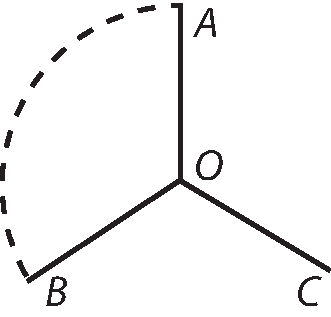
\includegraphics[width=0.2\textwidth]{images/LH035,14,02_119v-d1.pdf}\\
\centering [\textit{Fig. 7}]
\pend
\vspace{0.8em}
\pstart
\protect\setline{17} Interea \protect\setline{17}quod sequitur non est inelegans:
\edtext{Prop. X.
\textit{Contignationem\protect\index{Sachverzeichnis}{contignatio}
planam ex tignis\protect\index{Sachverzeichnis}{tignum} multo brevioribus,
quam sit areae longitudo invicem conjunctis construere.}%
}{\lemma{Prop. X. [...] \textit{construere}}\Cfootnote{%
\cite{00301}\textsc{J. Wallis}, \textit{Mechanica}, pars III, cap. 6, London 1670-1671, S. 589 (\cite{01008}\textit{WO} I, S. 953).\hspace{-3mm}}}
Jam quod adjicit,
\edtext{\textit{et computo aestimare},}{%
\lemma{\textit{et} [...] \textit{aestimare}}%
\Cfootnote{\cite{00301}a.a.O.\cite{01008}\hspace{-3mm}}}
huic non \edtext{fiderem. Explicatio: \textit{potest} }{%
\lemma{fiderem}\Bfootnote{%
\textit{(1)}\ posse
\textit{(2)}\ . Explicatio: \textit{potest}
\textit{L}}}%
%%%%%%%%%%%%%%%%%%%%%%%%%%%%%%%%%%%%%
\edtext{vero inquit \textit{hoc variis modis fieri.
Eam vero formam prae caeteris seligendam
putavi quam jam olim anno 1644
Cantabrigiae\protect\index{Ortsregister}{Cambridge}
primum delineabam, in Collegio Reginensi
in quo tum temporis socius eram,
et quam non ita multo post tigillis\protect\index{Sachverzeichnis}{tigillum} ligneis construendam curabam,
(quo manifestius indicarem, theoriam posse in praxin reduci);
eamque  in vesperiis Comitiorum Oxoniae\protect\index{Ortsregister}{Oxford},
anno 1652, postquam ad munus illud, quod etiamnum sustineo, vocatus eram,
solenni praelectione exponebam,
ejusque calculum\protect\index{Sachverzeichnis}{calculus}
vesperiis Comitiorum anni sequentis 1653 similiter explicabam.
Quamque ex eo tempore tum nostratium tum exterorum non pauci satis approbarunt,
aliqui etiam imitati sunt; quam et serenissimus Rex noster,
Carolus II,\protect\index{Namensregister}{\textso{Karl II.}, König von England 1660-1685}
post auspicatum suum in Angliam\protect\index{Ortsregister}{England} reditum,
inter} [\pgrk{keim'hlia}]\edtext{}{\lemma{\pgrk{khimeilia}}\Bfootnote{\textit{L ändert Hrsg.}}}
\textit{sua dignatus est reponere.
Specimen exhibet areae quadratae cujus latitudo
est fere quadrupla longitudinis tignorum\protect\index{Sachverzeichnis}{tignum} longissimorum,
quae ita sunt invicem intertexta, ut se mutuo sustineant.
Et quidem quo supra planitiem non assurgant,
qua parte tignum quodvis aliud sibi superne impositum sus\-tinet
(quod sui partibus intermediis fit)
superne ad mediam quasi partem excavatur,
qua parte vero alii impositum sustinetur,
quod in sui extremis fit, tantundem quasi excavatur inferne,
quo fit, ut sibi mutuo impacta aream planam faciant.}
%%%%%%%%%%%%%%%%%%%%%%%%%%%%%%%%%%%%%
\textit{Si tamen metuendum videatur ut} (+~dicendum, ne~+)
\textit{propter ligni\protect\index{Sachverzeichnis}{lignum} naturam flexilem
partes mediae onere pressae nonnihil}
%
\noindent
\textit{subsidant:
huic incommodo cavebitur, si excavationes non praecise ad mediam tigni crassitiem pertingant,
sed paulo citra medium desinant.
Quippe hoc pacto assurget paulum in singulis juncturis contignatio,\protect\index{Sachverzeichnis}{contignatio}
qua compensetur illa exigua depressio, quae ex curvatura oriatur.
Faciem lateralem tigni\protect\index{Sachverzeichnis}{tignum} longioris exhibet figura 244.
brevioris \edtext{figura 245, facies superna in ipsa fig. 243}{%
\lemma{figura 245,}\Bfootnote{%
\textit{(1)}\ figura
\textit{(2)}\ \textit{facies} [...] \textit{243}
\textit{L}}}
satis} patet.
}{\lemma{\textit{potest} [...] patet}\Cfootnote{\cite{00301}a.a.O., S.589f. (\cite{01008}\textit{WO} I, S. 953f).}} Sed haec non opus curiosius descri-
\pend
\pstart
\begin{wrapfigure}[7]{l}{0.25\textwidth} 
\vspace{-3.5mm}
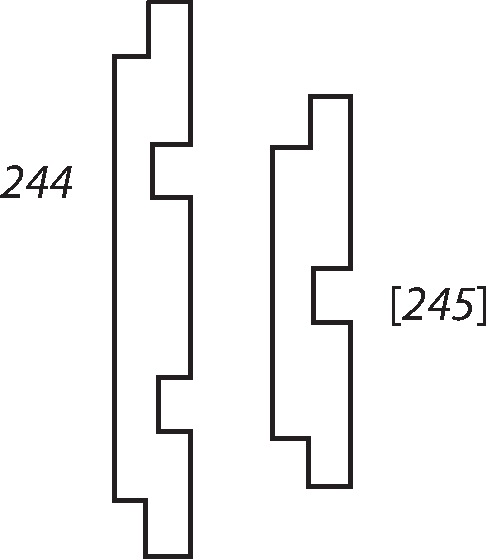
\includegraphics[trim = 0mm -4mm -10mm 0mm, clip, width=0.25\textwidth]{images/LH035,14,02_119v-d2}\\
\centering
[\textit{Fig. 8}]
\end{wrapfigure}
\noindent bere[,]
habetur enim \edtext{figura apud
\protect\index{Namensregister}{\textso{Monconys} (Monconisius), Balthasar de 1611-1665}%
Monconisium%
}{\lemma{figura apud Monconisium}\Cfootnote{\cite{00118}\textsc{B. de Monconys}, \textit{Journal des voyages}, Lyon 1665-1666, Teil II, S. 49f. und Fig. 8.}}%
\edtext{.\edtext{ Omissa putanda%
}{\lemma{Monconisium.}\Bfootnote{%
\textit{(1)}\ Omitte partem lineae 2 jungentem I et II lineas
\textit{(2)}\ Omissa putanda
\textit{L}}}
quae \edtext{lineis a me transfixa.%
}{\lemma{lineis}\Bfootnote{%
\textit{(1)}\ notata
\textit{(2)}\ a me transfixa
\textit{L}}}}{%
\lemma{Omissa [...] transfixa}%
\Cfootnote{Siehe die von Leibniz gezeichneten Verbindungsstriche in der Abbildung [\textit{Fig. 11}] auf S. \pageref{LH35,14,02_119v_ref-1}.}}
\edtext{%
Si \textit{area minus lata
ut paucioribus tignis de muro in murum} eatur,
\textit{eousque ut non nisi quaternis sit opus tignis ut in fig. 246
vel etiam, quae est figura omnium simplicissima,
ternis tignis, ut in fig. 247.}}{%
\lemma{\textit{Si area} [...] \textit{fig. 247}}\Cfootnote{\cite{00301}\textsc{Wallis}, \textit{Mechanica}, pars III, cap. 6, London 1670-1671, S. 591 (\cite{01008}\textit{WO} I, S. 954f.). Zitat mit Auslassungen.}}\edtext{}{\lemma{\hspace*{1,8mm}[\textit{Fig. 8}]}\killnumber\Cfootnote{\cite{00301}Vgl. a.a.O., Fig. 244 und 245 (\cite{01008}\textit{WO} I, S. 954).}}
\pend
% \vspace{0.85em}
%\pstart
%%\begin{wrapfigure}[13]{l}{0.29\textwidth} 
%\noindent
%\vspace{-4mm}
%\centering
%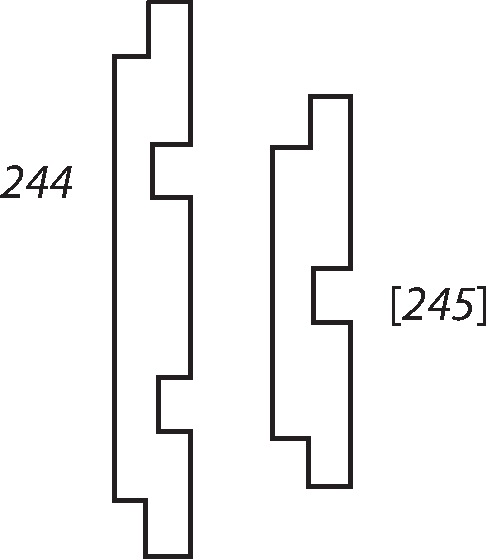
\includegraphics[trim = 0mm -4mm -4mm 0mm, clip, width=0.275\textwidth]{images/LH035,14,02_119v-d2}\\
%\noindent
%\centering
%[\textit{Fig. 8}]
%\vspace{-0.1mm}
%\edtext{}{\lemma{\hspace*{1,8mm}[\textit{Fig. 8}]}\killnumber\Cfootnote{\cite{00301}Vgl. a.a.O., Fig. 244 und 245 (\cite{01008}\textit{WO} I, S. 954).}}
%%\end{wrapfigure}
%\pend
%\newpage
%\pstart
%\vspace*{1.5em}
%\noindent\centering
%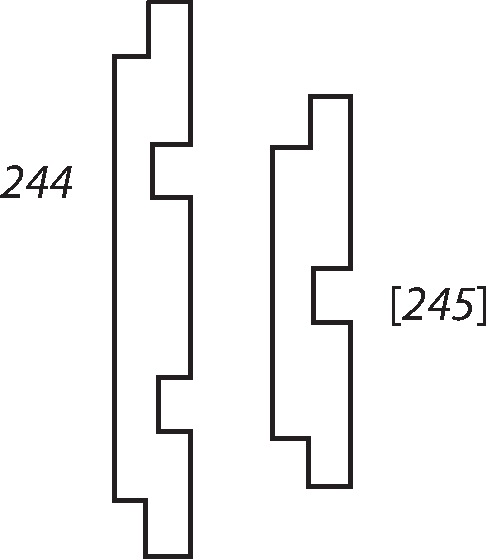
\includegraphics[width=0.3\textwidth]{images/LH035,14,02_119v-d2}\\%
%\vspace*{0.5em}%
%[\textit{Fig. 8}]\edtext{}{\lemma{\hspace*{1,8mm}[\textit{Fig. 8}]}\killnumber\Cfootnote{\cite{00301}Vgl. a.a.O., Fig. 244 und 245 (\cite{01008}\textit{WO} I, S. 954).}}
%\pend
%\newpage% PR: Rein provisorisch !!!!
\count\Bfootins=1200
\count\Cfootins=1200
\pstart
\begin{minipage}[t]{0.5\textwidth}
\hspace*{-5mm}
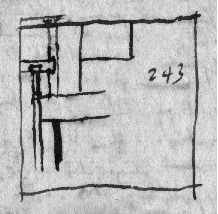
\includegraphics[width=0.7\textwidth]{images/LH035,14,02_119v_Ausschnitt.pdf}\\
%\vspace{0.3em}
\rule[-4mm]{0mm}{10mm}\noindent\centering\hspace*{-12mm}[\textit{Fig. 9}]
\end{minipage}
\hspace*{-5mm}
\begin{minipage}[t]{0.5\textwidth}
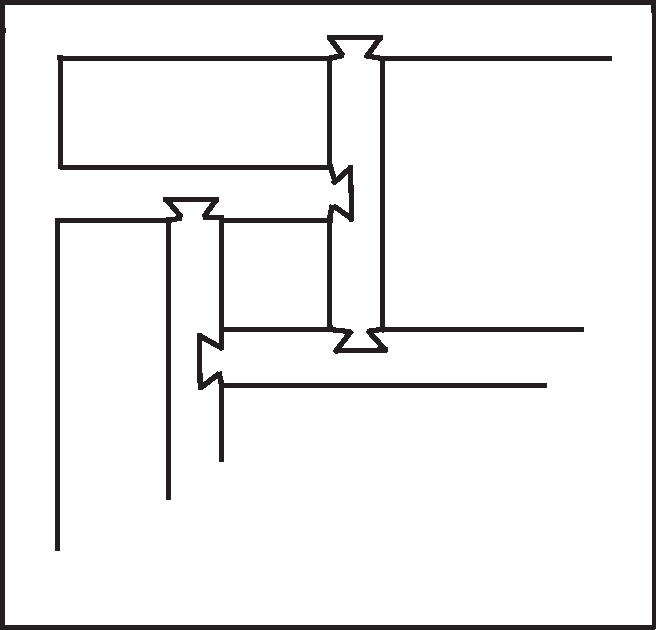
\includegraphics[width=0.7\textwidth]{images/LH035,14,02_119v-d3.pdf}\\
%\vspace{0.3em}
\rule[-4mm]{0mm}{10mm}\noindent\centering\hspace*{-6mm}[\textit{Fig. 10, erg. Hrsg. nach Wallis}]
% \vspace{1em}
\end{minipage}
%\hspace*{21mm} \textit{[Fig. 9]}\hspace*{59mm} \textit{[Fig. 10]}%
\edtext{}{\lemma{\hspace*{1,8mm}[\textit{Fig. 10}]}\killnumber\Cfootnote{Leibniz' Abzeichnung [\textit{Fig. 9}] nach Vorlage verbessert. Vgl. \cite{00301}a.a.O., Fig. 243 (\cite{01008}\textit{WO} I, S. 953).}}
\pend
\vspace*{4.5em}
%\vspace*{3em}% PR: Rein provisorisch !!!!
\pstart
\noindent\centering
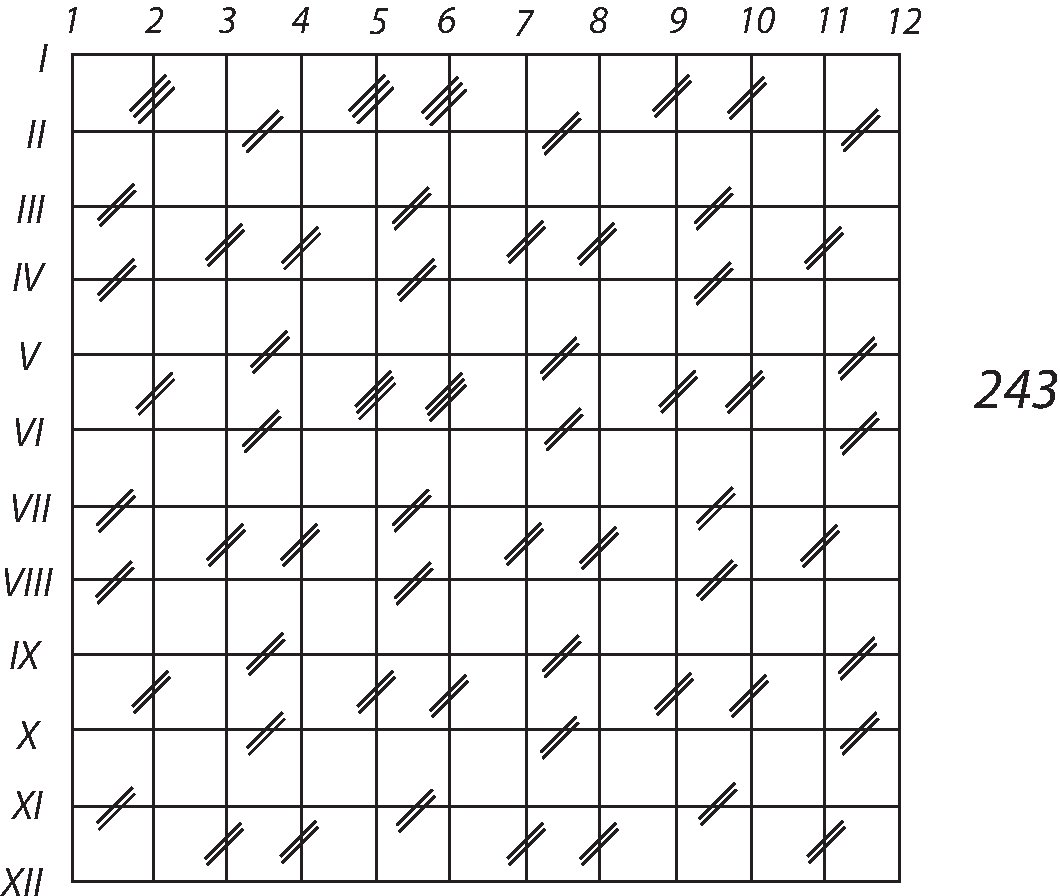
\includegraphics[width=0.6\textwidth]{images/LH035,14,02_119v-d4.pdf}\\%
%\vspace{1.0em}%
\rule[-4mm]{0mm}{10mm}\centering
[\textit{Fig. 11}]\edtext{}{\lemma{\hspace*{1,8mm}[\textit{Fig. 11}]}\killnumber\Cfootnote{\cite{00301}Vgl. a.a.O. %, Fig. 243 (\cite{01008}\textit{WO} I, S. 953).
Die Verbindungsstriche hat Leibniz ergänzt.}}\label{LH35,14,02_119v_ref-1}
\pend
\newpage % PR: Rein provisorisch !!!!
\pstart
%\vspace*{6em}
\begin{minipage}[t]{0.5\textwidth}
\hspace*{-10mm}
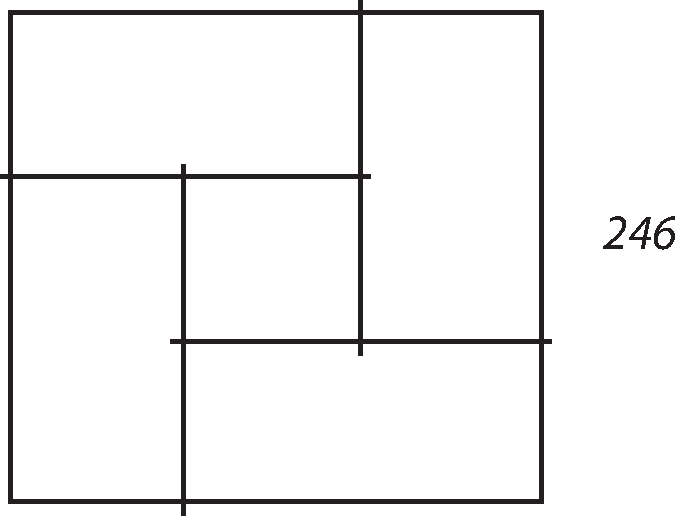
\includegraphics[width=0.8\textwidth]{images/LH035,14,02_119v-d5.pdf}\\
%\vspace{1.0em}
\rule[-4mm]{0mm}{10mm}\noindent\centering\hspace*{-20mm}[\textit{Fig. 12}]
\end{minipage}
\hspace*{-5mm}
\begin{minipage}[t]{0.5\textwidth}
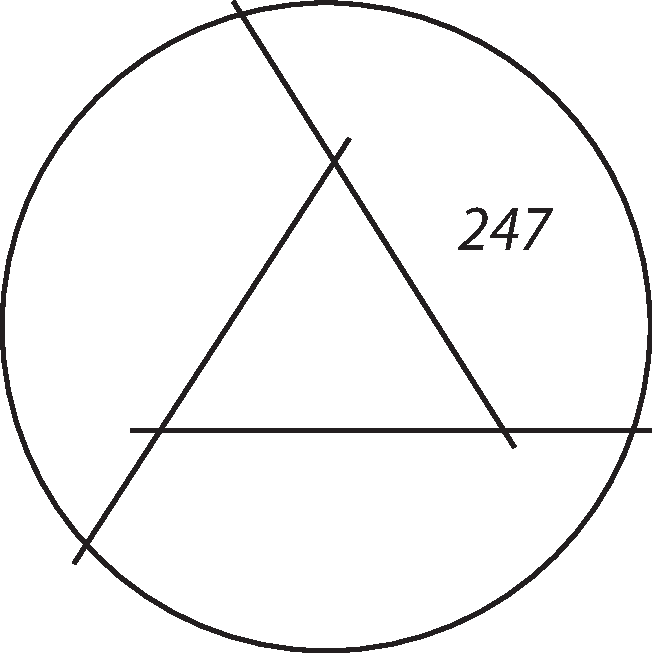
\includegraphics[width=0.60\textwidth]{images/LH035,14,02_119v-d6.pdf}\\
%\vspace{1.0em}
\rule[-4mm]{0mm}{10mm}\noindent\centering\hspace*{-6mm}[\textit{Fig. 13}]
% \vspace{1em}
\end{minipage}
\edtext{}{\lemma{\hspace*{1,8mm}[\textit{Fig. 12}]}\killnumber\Cfootnote{\cite{00301}Vgl. a.a.O., Fig. 246 (\cite{01008}\textit{WO} I, S. 955).}}%
\edtext{}{\lemma{\hspace*{1,8mm}[\textit{Fig. 13}]}\killnumber\Cfootnote{\cite{00301}Vgl. a.a.O., Fig. 247 (\cite{01008}\textit{WO} I, S. 955).}}%
\pend
\vspace{0.5em} 
%\newpage
\count\Afootins=1300
\count\Bfootins=1300
\count\Cfootins=1300
\pstart
%
[120~r\textsuperscript{o}] %%%%%%%%%%  HIER BEGINNT BLATT 120r.
%
\setline{1}In schol. ad cap. 7. prop. 3 disserit de rotis\protect\index{Sachverzeichnis}{rota}, quales curruum.\protect\index{Sachverzeichnis}{currus}
\edtext{\textit{Observatum est in usu communi,
quod et Aristoteles\protect\index{Namensregister}{\textso{Aristoteles}, 384-322 v. Chr.} attigit in Quaest. Mechan. 9,
majores rotas, sphaeras, cylindros facilius moveri.}}{%
\lemma{\textit{Observatum} [...] \textit{moveri}}\Cfootnote{%
\cite{00301}a.a.O., cap. 7, S. 617 (\cite{01008}\textit{WO} I, S. 973). Zitat mit Auslassung.
Siehe \textsc{Aristoteles}, \cite{01002}\textit{Mech.} 9, 852a14-16.% 
% \cite{00313}\textit{Quaestiones mechanicae}, Venedig 1585, S. 517.
}}
% 
\edtext{Cylindrum quali utimur in hortis ad complanandum[,]
\textit{scytalem vocat Aristoteles.}\protect\index{Namensregister}{\textso{Aristoteles}, 384-322 v. Chr.}}{%
\lemma{Cylindrum [...] \textit{Aristoteles}}\Cfootnote{%
\cite{00301}J. \textsc{Wallis}, \textit{Mechanica}, pars III, cap. 7, London 1670-1671, S. 618 (\cite{01008}\textit{WO} I, S. 974).
Siehe \textsc{Aristoteles}, \cite{01002}\textit{Mech.} 9, 852a16.}}
%
\edtext{\textit{Si aeris}\protect\index{Sachverzeichnis}{resistentia aeris}
(vel aquae\protect\index{Sachverzeichnis}{resistentia aquae})
\textit{resistentiae ratio habeatur}[,]
magis obsistetur majori.}{%
\lemma{\textit{Si aeris} [...] majori}\Cfootnote{%
\cite{00301}J. \textsc{Wallis}, \textit{Mechanica}, pars III, cap. 7, London 1670-1671, S. 618 (\cite{01008}\textit{WO} I, S. 974).}}
%
\edtext{Sed\edtext{ scabrities%
}{\lemma{Sed}\Bfootnote{%
\textit{(1)}\ cur rotam
\textit{(2)}\ scabrities
\textit{L}}}
soli potius advocanda.
Dentes\protect\index{Sachverzeichnis}{dens} impliciti ne labantur impedient[,]
non ut volvantur, unde rotunda moventur facilius.}{%
\lemma{Sed [...] facilius}\Cfootnote{%
\cite{00301}a.a.O., S. 618f. (\cite{01008}\textit{WO} I, S. 974).}}
\edtext{Hinc difficile trahuntur currus\protect\index{Sachverzeichnis}{currus} rotis\protect\index{Sachverzeichnis}{rota} sufflaminatis. 
Hinc fit etiam forte quod projecta\protect\index{Sachverzeichnis}{projectum} in aere\protect\index{Sachverzeichnis}{aer} volvuntur,
v.g. quae funda\protect\index{Sachverzeichnis}{funda} projiciuntur[,]
circulariter lata fuere antequam
\textit{relicta funda per circuli tangentem procedant,
projecti partes ab hujus circuli centro remotiores}[,]
\textit{majores propterea circumferentias eo motu descripserant 
adeoque velocioris motus conceperant impetum\protect\index{Sachverzeichnis}{impetus}
quam quae propiores,}
\textit{qui quidem impetus inaequales,
ubi ex peripheria ad rectam tangentem transitur volutionem inchoant
(projecti centro per rectam procedente partibusque superioribus concitatius reliquis)
\edtext{}{\lemma{}\Afootnote{\textit{Am Rand:} NB.\vspace{-8mm}}}%
eademque coepta cum nihil impediat perseverat.}}{%
\lemma{Hinc difficile [...] \textit{perseverat}}\Cfootnote{%
\cite{00301}a.a.O., S. 619 (\cite{01008}\textit{WO} I, S. 974f.). Zitat mit Auslassung.}}
%
Porro \edtext{%
\textit{quod facit in humi volutis soli asperitas\protect\index{Sachverzeichnis}{asperitas}
id facit in Trochlearum\protect\index{Sachverzeichnis}{trochlea} orbiculis 
asperitas funis}\protect\index{Sachverzeichnis}{funis}
[\textit{ductarii}],\edtext{}{\lemma{ductari}\Bfootnote{\textit{L ändert Hrsg. nach Vorlage}}}
% Wallis, Mechanica, London 1670-1671, S. 619.
quasi fingas non rotas sed fundum moveri.
Hinc facilius movetur funis
circa orbiculum mobilem.}{%
\lemma{\textit{quod} [...] mobilem}\Cfootnote{%
\cite{00301}a.a.O. 619 (\cite{01008}\textit{WO} I, S. 975). Zitat mit Auslassungen.}}
\pend 
\vspace{3em}
%\newpage
\pstart
\centering
%\protect\begin{wrapfigure}[9]{l}{0.4\textwidth}
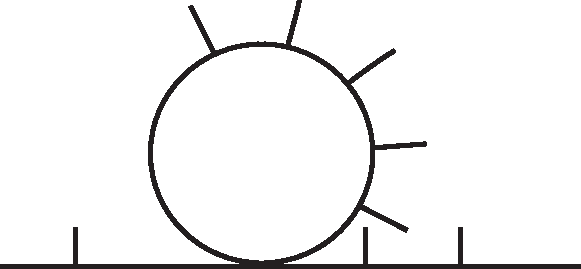
\includegraphics[trim = 0mm 0mm -5mm 0mm, clip, width=0.4\textwidth]{images/LH035,14,02_120r-d1.pdf}\\
\noindent \setline{6}
\rule[-4mm]{0mm}{10mm}\centering
[\textit{Fig. 14}]
\pend
\vspace{3em}
\pstart
%\protect\end{wrapfigure}
\begin{minipage}[c]{0.45\textwidth}
\hspace*{-10mm}
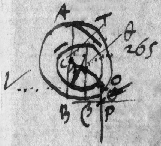
\includegraphics[width=0.9\textwidth]{images/LH035,14,02_120r-Ausschnitt.pdf}%\\
%\\
%\noindent\centering\hspace*{-18mm}[\textit{Fig. 15}]
\end{minipage}
\hspace*{-2mm}
\begin{minipage}[c]{0.55\textwidth}
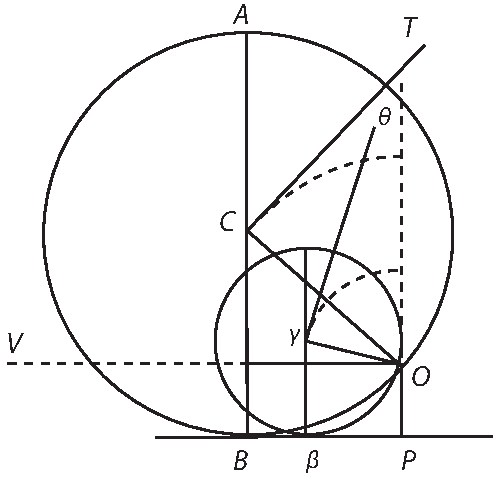
\includegraphics[width=0.95\textwidth]{images/LH035,14,02_120r-d2.pdf}%\\
%\\
%\noindent\centering\hspace*{-2mm}[\textit{Fig. 16, erg. Hrsg. nach Wallis}]
\vspace{0.5em}
\end{minipage}
\vspace*{1.0em}
\hspace*{17mm} [\textit{Fig. 15}]\hspace*{45mm}[\textit{Fig. 16, erg. Hrsg. nach Wallis}]%
\edtext{}{\lemma{\hspace*{1,8mm}[\textit{Fig. 16}]}\killnumber\Cfootnote{Leibniz' Abzeichnung [\textit{Fig. 15}] nach Vorlage verbessert. Vgl. \cite{00301}a.a.O., Fig. 265 (\cite{01008}\textit{WO} I, S. 974).}}%
\pend
\newpage
%\vspace{2em}
\count\Bfootins=1200
\count\Cfootins=1200
\pstart %%
\edtext{Si superandae sint in plano eminentiae,
acclivior erit ascensus per circuli minoris tangentem[,] ideo difficilior.
Et post ascensionem acclivem fingendum porro est,
circa extremum punctum seu apicem rotam\protect\index{Sachverzeichnis}{rota} volvi
\edtext{debere, ut porro%
}{\lemma{}\Bfootnote{\hspace{-2mm}debere,\ \textbar\ velut cum cycloeidem describere \textit{gestr.}\ \textbar\ debet, \textit{streicht Hrsg.}\ \textbar\ ut porro \textit{L}\hspace{-3mm}}}
progrediatur. 
[Imaginare]\edtext{}{\lemma{Imaginarre}\Bfootnote{\textit{L ändert Hrsg.}\hspace{-3mm}}}
jam rotae tantum centrum gravitatis\protect\index{Sachverzeichnis}{centrum gravitatis}
quod est ipsum circuli seu rotae centrum, volvi[;]
major obliquitas in \edtext{tangente $\displaystyle CT$ ad arcum circuli%
}{\lemma{tangente}\Bfootnote{%
\textit{(1)}\ ad $\displaystyle CT$ circuli
\textit{(2)}\ $\displaystyle CT$ ad
\textit{(a)}\ circulum
\textit{(b)}\ arcum circuli
\textit{L}\hspace{-3mm}}}
quem describit centrum majoris,
\edtext{quam $\displaystyle\gamma\theta$}{\lemma{}\Bfootnote{quam\ \textbar\ ad \textit{streicht Hrsg.}\ \textbar\ $\displaystyle\gamma\theta$\ \textit{L}}}
quem minoris.}{%
\lemma{Si superandae [...] minoris}%
\Cfootnote{\cite{00301}a.a.O., S. 620 (\cite{01008}\textit{WO} I, S. 975).}}
%
\edtext{Et forte ait nunc esse
\edtext{angulum $\displaystyle BCO,$ $\displaystyle \beta\gamma O$
\textit{quem vult Aristoteles}\protect\index{Namensregister}{\textso{Aristoteles}, 384-322 v. Chr.}%
}{\lemma{angulum}\Bfootnote{%
\textit{(1)}\ de quo loquitur Aristoteles\protect\index{Namensregister}{\textso{Aristoteles}, 384-322 v. Chr.}
\textit{(2)}\ $\displaystyle BCO$ [...] \textit{Aristoteles}
\textit{L}}}
\textit{cum dicit} 
\edtext{\textit{angulum circuli majoris habere nutum ad angulum circuli minoris}}{%
\lemma{\textit{angulum} [...] \textit{minoris}}%
\Cfootnote{\textsc{Aristoteles}, \cite{01002}\textit{Mech.} 8, 851b38f.%
% \cite{00313}\textit{Quaestiones mechanicae}, Venedig 1585, S. 516.
}} (quod male
\edtext{interpretes}{%
\lemma{interpretes}%
\Cfootnote{Wallis weist an dieser Stelle auf Henri de Monantheuil,\protect\index{Namensregister}{\textso{Monantheuil} (Monantholius), Henri 1536-1606} Bernardino Baldi\protect\index{Namensregister}{\textso{Baldi} (Baldus), Bernardino 1553-1617} und Giovanni di Guevara\protect\index{Namensregister}{\textso{Guevara} Giovanni de 1581-1641} hin.}}
ad angulum contactus\protect\index{Sachverzeichnis}{contactus} trahunt,)
\textit{nam et minor est angulus $\displaystyle BCO$ quam $\displaystyle \beta\gamma O.$
adeoque $\displaystyle C$ directius imminet,
et obliquior angulus}
[$\displaystyle COP$]\edtext{}{\lemma{$\displaystyle OP$}\Bfootnote{\textit{L ändert Hrsg.}}}
\textit{quam $\displaystyle \gamma OP.$
adeoque $\displaystyle C$ minus offensat,}
(:~\textit{si vero de angulo contactus\protect\index{Sachverzeichnis}{contactus} intelligeretur,
plus offensaret rota vel sphaera major quam minor
quia pluribus subjectis partibus simul incumbit
cylindrus seu sphaera materialis, ut post dicetur.}~:)
\textit{Sive igitur superanda sit sive deprimenda eminentia $\displaystyle PO,$
quorum ut plurimum vel alterum vel utrumque faciendum erit,
quo volutio continuetur,
magis valebit rota major caeteris paribus.
% [...]
Sin abrumpenda esset eminentia $\displaystyle PO$ vel propellenda:
cum hoc per pulsum lateralem faciendum sit,
et potissimum in horizontali recta
ut $\displaystyle VO$ secundum quam vel huic parallelam fit tractio horizontalis}[,]
\textit{quae magis hic spectanda quam perpendicularis pressio,
id potius fiet per rectam $\displaystyle \gamma O$
quae a situ horizontali minus recedit, quam per $\displaystyle CO.$
Adeoque hoc respectu Rota minor praevalebit majori},
sed \textit{hoc rarius contingit,
et vix nisi in altioribus obstaculis.
Eminentiae minores deprimi solent vel superari potius quam propelli.}}{%
\lemma{Et forte [...] \textit{propelli}}%
\Cfootnote{\cite{00301}a.a.O., S. 621 (\cite{01008}\textit{WO} I, S. 976). Zitat mit Auslassungen.}}
%
\pend
\pstart
\edtext{Est et alia Ratio pro majore. \textit{Dum ab eminentia una}
[\textit{ad}]\edtext{}{\lemma{ab}\Bfootnote{\textit{L ändert Hrsg.}}}
\textit{alteram transit magis deprimitur minor quam major rota},
et ideo ei ex profundiori valle assurgendum.
Est et alia ratio[:] si rota\protect\index{Sachverzeichnis}{rota} minor aeque gravis
\edtext{majori, Rota minor deprimat planitiem%
}{\lemma{majori,}\Bfootnote{%
\textit{(1)}\ majus ejus segmentum
\textit{(2)}\ quod intra terram lutumque imprimetur rota minore, majus erit quam quod majore
\textit{(3)}\ Rota [...] planitiem
\textit{L}}}
$\displaystyle NVO$ usque ad $\displaystyle B$ vel $\displaystyle \beta.$
Ergo subjectae materiae\protect\index{Sachverzeichnis}{materia} tantum loco pellet,
\edtext{quo}{\lemma{quo}\Cfootnote{In der Vorlage \textit{quantum}.}}
locum faciat segmento $\displaystyle QRB.$
\textit{Quo autem major eo}
\edtext{\textit{penetret} tantum \textit{deprimendum erit seu loco pellendum,
quantum est segmentum $\displaystyle NBO,$
quod majus segmento $\displaystyle QBR.$}%
}{\lemma{\textit{penetret}}\Bfootnote{%
\textit{(1)}\ \textit{tantundem} quo autem major eo pen
\textit{(2)}\ tantum [...] $\displaystyle QBR.$
\textit{L}}}
\textit{Hoc} ergo \textit{ut fiat majore opus est pondere.
Ponitur autem utrique pondus\protect\index{Sachverzeichnis}{pondus} aequale,
non} ergo \textit{fiet},
ergo major tam alte non penetrabit.}{%
\lemma{Est et [...] penetrabit}%
\Cfootnote{\cite{00301}J. \textsc{Wallis}, \textit{Mechanica}, pars III, cap. 7, London 1670-1671, S. 622 (\cite{01008}\textit{WO} I, S. 976f.).}}
%
\edtext{Hactenus rotam\protect\index{Sachverzeichnis}{rota} consideravimus ut gravem,
at seclusa quoque gravitatis\protect\index{Sachverzeichnis}{gravitas} consideratione idem habet locum.
In superiore \edtext{figura, 265}{\lemma{figura, 265}\Cfootnote{Siehe oben, [\textit{Fig. 15}] und [\textit{Fig. 16}].}}
amoliendus \edtext{obex\protect\index{Sachverzeichnis}{obex} $\displaystyle OP.$%
}{\lemma{obex}\Bfootnote{%
\textit{(1)}\ 265.
\textit{(2)}\ $\displaystyle OP.$
\textit{L}}}
vis\protect\index{Sachverzeichnis}{vis} applicata in $\displaystyle A,$
vel ut in cylindris plerumque aut rotis,
in $\displaystyle C.$ fulcrum\protect\index{Sachverzeichnis}{fulcrum}
vectis\protect\index{Sachverzeichnis}{vectis}
[$\displaystyle AB.$]\edtext{}{\lemma{$\displaystyle B.$}\Bfootnote{\textit{L ändert Hrsg. nach Vorlage}}}
Fortius ergo aget applicata in $\displaystyle C.$
quam in $\displaystyle \gamma.$}{%
\lemma{Hactenus [...]  quam in $\displaystyle \gamma$}%
\Cfootnote{\cite{00301}a.a.O., S. 622f. (\cite{01008}\textit{WO} I, S. 977).}}
\pend
\count\Bfootins=1200
\count\Cfootins=1200
% \newpage% PR: Rein provisorisch !!!!
\vspace*{1.5em}
\pstart
\noindent\centering
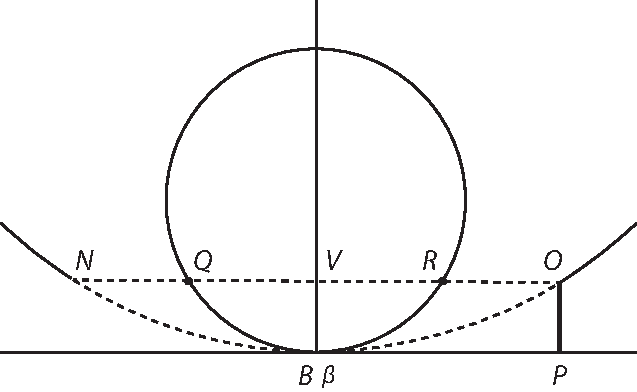
\includegraphics[width=0.6\textwidth]{images/LH035,14,02_120r-d3.pdf}\\%
\rule[-4mm]{0mm}{10mm}\setline{8}%
[\textit{Fig. 17}]\edtext{}{\lemma{\hspace*{1,8mm}[\textit{Fig. 17}]}\killnumber\Cfootnote{\cite{00301}Siehe a.a.O., Fig.
% 266 und 
267 (\cite{01008}\textit{WO} I, S. 976).}}
\pend
%\newpage% PR: Rein provisorisch !!!!
\vspace*{1em}% PR: Rein provisorisch !!!!
%%%%%%%%%%%%%%%%%%%% 
\pstart
\edtext{Quod attinet ad funes\protect\index{Sachverzeichnis}{funis} ductarios
et trochlearum\protect\index{Sachverzeichnis}{trochlea} orbiculos[,]
premitur orbiculus contra axem a fune[,] 
hinc frictio.\protect\index{Sachverzeichnis}{frictio}
Et quo axis\protect\index{Sachverzeichnis}{axis} major hoc et frictio.
Hinc in \edtext{majoribus orbiculis}{%
\lemma{}\Afootnote{\textit{Über} majoribus orbiculis: ex Baldo\textsuperscript{[a]}%
\vspace{2mm}\\
\footnotesize
\textsuperscript{[a]} ex Baldo: B.\cite{01005} \textsc{Baldi}, \textit{In mechanica Aristotelis problemata exercitationes}, Mainz 1621, S. 78-80.
\vspace{-4mm}
}}
minor ratio axis, ad circumferentiam orbis,
ideoque frictionis quae
\edtext{in ea}{\lemma{in ea}\Bfootnote{\textit{erg. L}}}
fieret manente orbiculo ob resistentiam
\edtext{axis; praesertim cum%
}{\lemma{axis;}\Bfootnote{%
\textit{(1)}\ contra ips
\textit{(2)}\ praesertim cum
\textit{L}}}
et vis ad majorem a centro motus distantiam applicetur.
\edtext{}{\lemma{}\Afootnote{\textit{Über} applicetur: v. c.}}%
Eadem in plaustrorum curruumve rotis.
\textit{Nam axium extrema quae rotarum\protect\index{Sachverzeichnis}{rota} modiolis immittuntur,
onera pressa, ita premunt foraminum imo,
ut non possit sine frictione converti rota circa axem suum,
in parte praesertim inferiori.
Quam causam assignat Arist.\protect\index{Namensregister}{\textso{Aristoteles}, 384-322 v. Chr.}
Mech. Q. 11.}
\edtext{\textit{cur supra scytalas
% [...]
facilius} moventur \textit{onera\protect\index{Sachverzeichnis}{onus} quam supra currus}[,]}{%
\lemma{\textit{cur} [...] \textit{currus}}%
\Cfootnote{\textsc{Aristoteles}, \cite{01002}\textit{Mech.} 11, 852a29f.%
% \cite{00313}\textit{Quaestiones mechanicae}, Venedig 1585, S. 517.
}}
\textit{nempe ob evitatam axis\protect\index{Sachverzeichnis}{axis} frictionem.}}{%
\lemma{Quod [...] \textit{frictionem}}%
\Cfootnote{\cite{00301}a.a.O., S. 624 (\cite{01008}\textit{WO} I, S. 978). Zitat mit Auslassungen.}}
%
\pend
\count\Bfootins=1500
\count\Cfootins=1500
\pstart
\edtext{Est et alia ratio a frictione\protect\index{Sachverzeichnis}{frictio}
quae \edtext{favet majoribus rotis%
}{\lemma{favet}\Bfootnote{%
\textit{(1)}\ curribus\protect\index{Sachverzeichnis}{currus}
\textit{(2)}\ majoribus rotis
\textit{L}}}
vel orbiculis, sumta et ipsa a frictione.
%
[120~v\textsuperscript{o}] %%%%%%%%%%  HIER BEGINNT BLATT 120v.
%
Posita nimirum eadem utrobique axis magnitudine[,]
non tantum difficilius superabitur hoc frictionis\protect\index{Sachverzeichnis}{frictio}
impedimentum in axe,\protect\index{Sachverzeichnis}{axis}
in minoribus rotis,\protect\index{Sachverzeichnis}{rota}
sed etiam saepius repetetur,
quia ut aequale spatium percurrat rota minor, saepius convertetur.
Hinc et plaustrorum rotae anteriores et axes citius teruntur et saepius
\edtext{reparantur. Cui tamen conferre potest,%
}{\lemma{reparantur.}\Bfootnote{%
\textit{(1)}\ Accedit
\textit{(2)}\ Cui [...] potest
\textit{L}}}
quod quia [inferiores]\edtext{}{\lemma{inferior}\Bfootnote{\textit{L ändert Hrsg.}}}
plerumque esse solent rotae anteriores magis a pondere premuntur.}{%
\lemma{Est et [...] premuntur}%
\Cfootnote{\cite{00301}J. \textsc{Wallis}, \textit{Mechanica}, pars III, cap. 7, London 1670-1671, S. 625 (\cite{01008}\textit{WO} I, S. 978).}}
%
\pend
\pstart
\edtext{Cur plaustrorum rotae anteriores posterioribus minores?
Ratio quia ob viarum flexus saepe plaustrum vertendum,
cui multum conducit rotarum\protect\index{Sachverzeichnis}{rota} anteriorum parvitas.
Magno opus foret circuitu si
\edtext{aequales essent anteriores posterioribus.%
}{\lemma{aequales}\Bfootnote{%
\textit{(1)}\ minores majoribus
\textit{(2)}\ essent anteriores posterioribus.
\textit{L}}}
Sed est et alia ratio.
Notandum \textit{lora quae plaustris equum alligant
affixa esse saltem mediate ad axem anteriorem ejusve capita,
saltem non inferius quam sit axis ille.}
Si axis\protect\index{Sachverzeichnis}{axis} ille aequalis pectori equi[,]
[tractus]\edtext{}{\lemma{tractatus}\Bfootnote{\textit{L ändert Hrsg. nach Vorlage}}}
erit horizontalis seu recta $\displaystyle BC$ horizonti parallela[;]
sed cum ascendendum, tunc $\displaystyle BC$ recta
secundum quam vis\protect\index{Sachverzeichnis}{vis} applicatur[,]
parallela fiet potius $\displaystyle TO$ acclivitati.
Saltem propius ei accedet, quam si $\displaystyle B$ punctum
esset aeque altum ac $\displaystyle C$ pectus equi, vel etiam altius.}{%
\lemma{Cur [...] altius}%
\Cfootnote{\cite{00301}a.a.O., S. 626f. (\cite{01008}\textit{WO} I, S. 979f.).}}
%
\pend
%\vspace*{2.5em}
\newpage
\pstart
% \vspace*{3em}
\noindent\centering
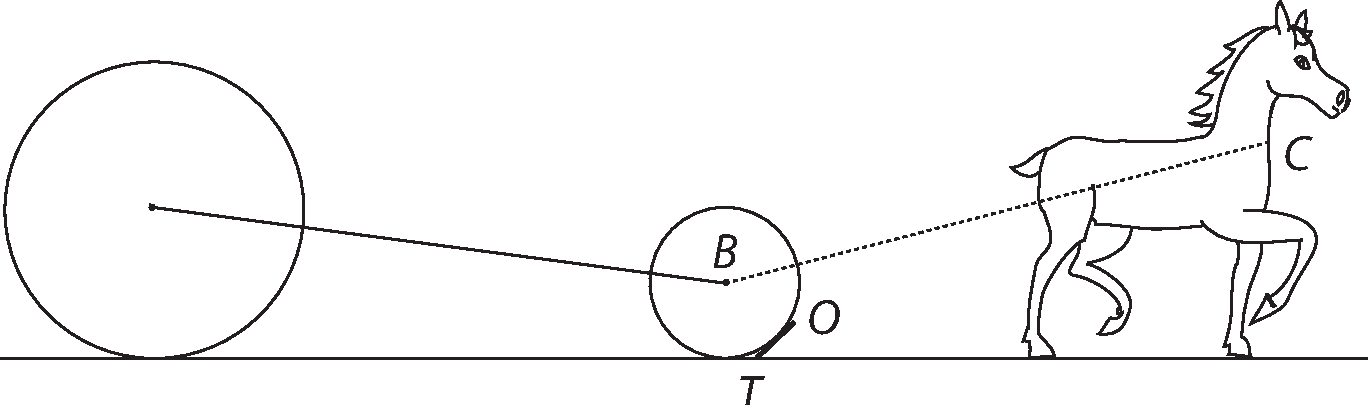
\includegraphics[width=0.90\textwidth]{images/LH035,14,02_120v-d1.pdf}\\%
\vspace*{0.5em}%
[\textit{Fig. 18}]\edtext{}{\lemma{\hspace*{1,8mm}[\textit{Fig. 18}]}\killnumber\Cfootnote{Vgl. \cite{00301}a.a.O., Fig. 271 (\cite{01008}\textit{WO} I, S. 979).}}
\pend
\vspace{3em}
\count\Afootins=1200
\count\Bfootins=1200
\count\Cfootins=1200
\pstart
\textso{Cap. IX. de Cochlea. }\protect\index{Sachverzeichnis}{cochlea}%
\setline{1}\edtext{%
\textit{Helix circa Cylindrum rectum est curva similaris sive uniformis,
cujus pars}
quaevis cuivis congruere potest.
\textit{Si expandi intelligatur in planum superficies cylindrica,}
ex helice\protect\index{Sachverzeichnis}{helix} \textit{fiet linea}
\edtext{\textit{recta}, et talis quidem%
}{\lemma{\textit{recta},}\Bfootnote{%
\textit{(1)}\ ita
\textit{(2)}\ et talis quidem
\textit{L}}}
ut qui prius maneant inclinationis et obliquitatis anguli.}{%
\lemma{\textit{Helix} [...] anguli}%
\Cfootnote{\cite{00301}a.a.O., cap. 9, prop. 1, S. 638 (\cite{01008}\textit{WO} I, S. 988).}}
%
\edtext{Quae duae posteriores proprietates competunt et spiralibus circa cylindros scalenos,
aut etiam circa solidum prismaticum quodvis.
Sed non prima.
Ex similari helicis natura pendet usus cochlearum.}{%
\lemma{Quae [...] cochlearum}%
\Cfootnote{\cite{00301}a.a.O., S. 639 (\cite{01008}\textit{WO} I, S. 988).}}
%
\pend
\pstart
\edtext{Spiralis\protect\index{Sachverzeichnis}{spiralis}
circa cylindrum rectum vel scalenum,
vel etiam solidum prismaticum quodvis,
longitudinem exhibere.
Nimirum expansa superficie in planum in rectam ei aequalem transit,
cujus datur longitudo.}{%
\lemma{Spiralis [...] longitudo}%
\Cfootnote{\cite{00301}a.a.O., prop. 5, S. 642 (\cite{01008}\textit{WO} I, S. 990).}}
%
\edtext{Nempe pro una circulatione,
ejus quadratum aequale quadrato altitudinis cylindri et
\edtext{curvae quae est basis.%
}{\lemma{curvae}\Bfootnote{%
\textit{(1)}\ baseos
\textit{(2)}\ quae est basis
\textit{L}}}}{%
\lemma{Nempe [...] basis}%
\Cfootnote{\cite{00301}a.a.O., prop. 6, S. 643f. (\cite{01008}\textit{WO} I, S. 990).}}
%
Subtilis est satis
\edtext{methodus quam subjicit,
qua exhibet cochleae\protect\index{Sachverzeichnis}{cochlea} soliditatem,
cujuscunque generis sit prisma.
Scilicet \textit{non modo prisma scalenum utcunque inclinatum sed et utcunque distortum
aequatur prismati recto aeque alto.}}{%
\lemma{methodus [...] \textit{alto}}%
\Cfootnote{\cite{00301}a.a.O., S. 644 (\cite{01008}\textit{WO} I, S. 991).}}
% 
\pend
\newpage
%\vspace*{3em}% PR: Rein provisorisch !!!!
\pstart
\begin{minipage}[t]{0.5\textwidth}
\hspace*{-10mm}
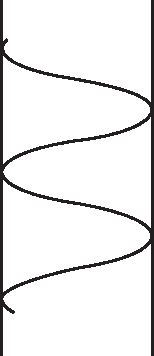
\includegraphics[width=0.3\textwidth]{images/LH035,14,02_120v-d2.pdf}\\
\\
\noindent\centering\hspace*{-29mm}[\textit{Fig. 19}]
\end{minipage}
\hspace*{-5mm}
\begin{minipage}[t]{0.5\textwidth}
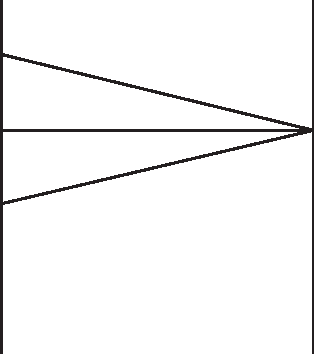
\includegraphics[width=0.6\textwidth]{images/LH035,14,02_120v-d3.pdf}\\
\\
\noindent\centering\hspace*{-9mm}[\textit{Fig. 20}]
\vspace{1em}
\end{minipage}
%\hspace*{22mm}[\textit{Fig. 19}] \hspace*{46mm}[\textit{Fig. 20}]
\pend
%\newpage
\count\Afootins=1000
\count\Bfootins=1000
\count\Cfootins=1000
\vspace*{2.0em}% PR: Rein provisorisch !!!!
\pstart 
Cap. X. \setline{1}de motu accelerato\protect\index{Sachverzeichnis}{motus acceleratus} etc.
% Wallis, Mechanica, London 1670-1671, S. 645.
\edtext{\textit{Si celeritates\protect\index{Sachverzeichnis}{celeritas} sint in temporum ratione duplicata
erunt longitudines in temporum\protect\index{Sachverzeichnis}{tempus} ratione triplicata} etc.
\textit{Si celeritates in ratione temporum triplicata}[,]
\textit{erunt longitudines in quadruplicata} etc.}{%
\lemma{\textit{Si celeritates} [...] \textit{quadruplicata} etc.}%
\Cfootnote{\cite{00301}a.a.O., cap. 10, prop. 5, S. 653 (\cite{01008}\textit{WO} I, S. 997). Zitat mit Aus\-lassungen\hspace{-2mm}}}
\pend
\pstart 
\edtext{Motus projectorum\protect\index{Sachverzeichnis}{motus proejctorum}
in parabolica:\protect\index{Sachverzeichnis}{linea parabolica}
exclusa consideratione resistentis medii.}{%
\lemma{Motus [...] medii}%
\Cfootnote{\cite{00301}a.a.O., prop. 8, S. 658 (\cite{01008}\textit{WO} I, S. 1001).}}
%
\edtext{\textit{Quoniam ob hanc resistentiam\protect\index{Sachverzeichnis}{resistentia medii}
Motus secundum directionem projicientis,
qui supponitur aequabilis}[,]
\textit{revera minuitur et denique extinguitur,
ob continuam cum medio resistente luctam,
et propterea sensim deficit a linea parabolica.}
Et hinc fit etiam, ut
[globuli ex bombardis]\edtext{}{\lemma{globuli ex bombardis}\Bfootnote{\textit{erg. Hrsg. nach Vorlage}}}
ex majore distantia minus feriant.
Nam si uniformi celeritate\protect\index{Sachverzeichnis}{celeritas uniformis} procederet
[latio]\edtext{}{\lemma{latio}\Bfootnote{\textit{erg. Hrsg. nach Vorlage}}}
secundum directionem projicientis,
quicquid sit de motu descensus[,]
murum sive propinquum sive remotum aequaliter feriret.}{%
\lemma{\textit{Quoniam} [...] feriret}%
\Cfootnote{\cite{00301}a.a.O., S. 659 (\cite{01008}\textit{WO} I, S. 1001).}}
%
\pend
\vspace*{1.0em}
\pstart
Cap. XI. de percussione.\protect\index{Sachverzeichnis}{percussio}
\edtext{%
\textit{Si grave\protect\index{Sachverzeichnis}{grave} subsequens
segnius secundum eandem rectam praecedenti directe impingat},
si \textit{utriusque momentum\protect\index{Sachverzeichnis}{momentum}
per utriusque pondus\protect\index{Sachverzeichnis}{pondus} dividatur}[,]
\textit{habebitur communis utriusque celeritas},
et \textit{celeritas futura in utriusvis pondus ducta exhibet ejus momentum} mox \textit{futurum.}}{%
\lemma{\textit{Si grave} [...] \textit{futurum}}%
\Cfootnote{\cite{00301}a.a.O., cap. 11, prop. 3, S. 664 (\cite{01008}\textit{WO} I, S. 1004). Zitat mit Auslassung.}}
%
\pend
\newpage
\count\Afootins=1200
\count\Bfootins=1200
\count\Cfootins=1200
\pstart
\edtext{%
\textit{Si contrariis motibus sibi impingant}[,]
\textit{Momentorum} non summa
sed \textit{differentia per summam ponderum dividatur.}}{%
\lemma{\textit{Si contrariis} [...] \textit{dividatur}}%
\Cfootnote{\cite{00301}a.a.O., prop. 4, S. 665 (\cite{01008}\textit{WO} I, S. 1005). Zitat mit Auslassung.}}
%
\pend
\pstart
\edtext{%
\textit{Ictus magnitudo aequipollet
\edtext{duplo momenti}{\lemma{}\Afootnote{\textit{Über duplo momenti:} Obscure.\vspace{-8mm}}}
ablati in fortiori.}
Facit scilicet tum ut fortius perdit,
tum ut alterum recipiat.
\textit{Designo autem ictus\protect\index{Sachverzeichnis}{ictus} magnitudinem per momentum fortiori
ablatum quoniam effectus ictus in fortiori} semper \textit{uniformis}[,]
sola scilicet momenti ablatio[,]
\textit{adeoque simplicius verbis exprimitur,
effectus\protect\index{Sachverzeichnis}{effectus} in reliquo}
nunc \textit{impetus\protect\index{Sachverzeichnis}{impetus} deperditio,}
nunc \edtext{\textit{aquisitio novi, nonnunquam utrumque}.%
}{\lemma{\textit{aquisitio}}\Bfootnote{%
\textit{(1)}\ \textit{novi} etc.
\textit{(2)}\ \textit{novi, nonnunquam utrumque.}
\textit{L}}}}{%
\lemma{\textit{Ictus} [...] \textit{utrumque}}%
\Cfootnote{\cite{00301}a.a.O., prop. 5, S. 666f. (\cite{01008}\textit{WO} I, S. 1006). Zitat mit Auslassung.\hspace{25mm}}}
%
\pend
\pstart
\edtext{%
Hinc sequitur si obex\protect\index{Sachverzeichnis}{obex} sit firmus[,]
\textit{ictum\protect\index{Sachverzeichnis}{ictus} aequipollere
duplo momento\protect\index{Sachverzeichnis}{momentum} gravis impingentis,}
nam totum perdit}{%
\lemma{Hinc [...] perdit}%
\Cfootnote{\cite{00301}a.a.O., prop. 6, S. 667 (\cite{01008}\textit{WO} I, S. 1006f.).}}%
%
.\edtext{%
\newline%
\hspace*{7,5mm}%
Idem est si gravia\protect\index{Sachverzeichnis}{grave}%
}{\lemma{perdit.}\Bfootnote{%
\textit{(1)}\ Si gravia
\textit{(2)}\ Idem est si gravia
\textit{L}}}%
\edtext{ celeritatibus\protect\index{Sachverzeichnis}{celeritas} reciproce proportionalibus
[sibi]\edtext{}{\lemma{sibi}\Bfootnote{\textit{erg. Hrsg. nach Vorlage}}}
occurrant, nam et tunc destruitur ictus.}{%
\lemma{Idem [...] ictus}%
\Cfootnote{\cite{00301}a.a.O., prop. 7, S. 668 (\cite{01008}\textit{WO} I, S. 1007).}}
%\newpage
%\pstart
%\edtext{%
%Hinc sequitur si obex\protect\index{Sachverzeichnis}{obex} sit firmus[,]
%\textit{ictum\protect\index{Sachverzeichnis}{ictus} aequipollere
%duplo momento\protect\index{Sachverzeichnis}{momentum} gravis impingentis,}
%nam totum perdit}{%
%\lemma{Hinc [...] perdit}%
%\Cfootnote{\cite{00301}a.a.O., prop. 6, S. 667 (\cite{01008}\textit{WO} I, S. 1006f.).}}%
%%
%\edtext{.\edtext{ \\%
%\hspace*{7,5mm}%
%Idem est si gravia\protect\index{Sachverzeichnis}{grave}%
%}{\lemma{perdit.}\Bfootnote{%
%\textit{(1)}\ Si gravia
%\textit{(2)}\ Idem est si gravia
%\textit{L}}}
%celeritatibus\protect\index{Sachverzeichnis}{celeritas} reciproce proportionalibus
%[sibi]\edtext{}{\lemma{sibi}\Bfootnote{\textit{erg. Hrsg. nach Vorlage}}}
%occurrant, nam et tunc destruitur ictus.}{%
%\lemma{Idem [...] ictus}%
%\Cfootnote{\cite{00301}a.a.O., prop. 7, S. 668 (\cite{01008}\textit{WO} I, S. 1007).}}
%
(+~Ratio quia destruuntur duo motus, concurrentes aequales.
Hinc duplum momenti deperditi.~[+)]\edtext{}{\lemma{\phantom(\hspace{-1.2mm}+)}\Bfootnote{\textit{erg. Hrsg.}}}
\pend
\pstart
\edtext{%
\textit{Si grave motum aequali quiescenti non impedito directe impingat,
ictus magnitudo momento gravis moti aequipollet.}}{%
\lemma{\textit{Si grave} [...] \textit{aequipollet}}%
\Cfootnote{\cite{00301}a.a.O., prop. 9, S. 670 (\cite{01008}\textit{WO} I, S. 1008).}}
%
\pend
\pstart
\edtext{%
\textit{Si duo gravia aequalia, celeritatibus inaequalibus in easdem partes ferantur,
et sequens antecedenti directe impingat,
ictus aequipollet momento utriusvis,
celeritatum differentia lati.}}{%
\lemma{\textit{Si duo} [...] \textit{lati}}%
\Cfootnote{\cite{00301}a.a.O., prop. 10, S. 671 (\cite{01008}\textit{WO} I, S. 1008).}}
%
\pend
\pstart
\edtext{%
\textit{Si duo gravia}
[\textit{aequalia}]\edtext{}{\lemma{\textit{aequalia}}\Bfootnote{\textit{erg. Hrsg. nach Vorlage}}}
\textit{celeritatibus utcunque inaequalibus ad contrarias partes lata sibi mutuo directe occurrant,
ictus\protect\index{Sachverzeichnis}{ictus} aequipollet momento}\protect\index{Sachverzeichnis}{momentum}
\edtext{utriusque[,]}{\lemma{utriusque}\Cfootnote{In der Vorlage \textit{utriusvis}.\hspace{-2mm}}}
\edtext{\textit{celeritatum aggregato lati.}%
}{\lemma{\textit{celeritatum}}\Bfootnote{%
\textit{(1)}\ differentia \textit{lati}
\textit{(2)}\ \textit{aggregato lati}
\textit{L}}}}{%
\lemma{\textit{Si duo} [...] \textit{lati}}%
\Cfootnote{\cite{00301}a.a.O., prop. 11, S. 672 (\cite{01008}\textit{WO} I, S. 1009).}}
%
\pend
\pstart
\edtext{%
\textit{Si grave\protect\index{Sachverzeichnis}{grave} motum gravi quiescenti utcunque inaequali directe impingat;
erit ictus magnitudo, ad momentum gravis moti, ut quiescentis pondus\protect\index{Sachverzeichnis}{pondus} duplum,
ad ponderis utriusque aggregatum.}}{%
\lemma{\textit{Si grave} [...] \textit{aggregatum}}%
\Cfootnote{\cite{00301}a.a.O., prop. 12, S. 673 (\cite{01008}\textit{WO} I, S. 1009).}}
%
\pend
\count\Afootins=1000
\count\Bfootins=1000
\count\Cfootins=1000
\newpage
\pstart
\edtext{%
Si\edtext{ sequens grave%
}{\lemma{Si}\Bfootnote{%
\textit{(1)}\ duo gravia
\textit{(2)}\ sequens grave
\textit{L}}}
\textit{antecedenti directe impingat,
erit ictus magnitudo ad momentum gravis sequentis celeritatum differentia lati,
ut duplum ponderis antecedentis ad simul utriusque pondus:
ad momentum vero antecedentis eadem celeritatum differentia lati,
ut duplum sequentis ad simul utriusque pondus,
hoc est, ad momentum utriusvis differentia celeritatum lati,
ut duplum reliqui ad simul utriusque pondus.}}{%
\lemma{Si sequens [...] \textit{pondus}}%
\Cfootnote{\cite{00301}a.a.O., prop. 13, S. 674 (\cite{01008}\textit{WO} I, S. 1010).}}
%
\pend
\pstart
\edtext{%
\textit{Si duo gravia aequalia vel inaequalia
quibuscunque celeritatibus, motibus contrariis sibi mutuo directe occurrant,
erit ictus magnitudo ad momentum alterutrius gravium,
ut reliqui pondus duplum, ad simul utriusque pondus.}}{%
\lemma{\textit{Si duo} [...] \textit{pondus}}%
\Cfootnote{\cite{00301}a.a.O., prop. 14, S. 675 (\cite{01008}\textit{WO} I, S. 1011). Zitat mit Auslassung.}}
%
\pend
%\newpage
\pstart
Quod\edlabel{LH35,14,02_121r_ref-1} attinet ad horum
%
[121~r\textsuperscript{o}] %%%%%%%%%%  HIER BEGINNT BLATT 121r.
%
Theorematum \edtext{demonstrationes facile apparet}{%
\lemma{demonstrationes}\Bfootnote{%
\textit{(1)}\ in prop. 2 statim supponit quod scilicet
\textit{(2)}\ facile apparet
\textit{L}}}
rigorose examinanti
\edtext{ab eo non demonstrari caput rei,}{%
\lemma{ab eo}\Bfootnote{%
\textit{(1)}\ pleraque
\textit{(2)}\ non demonstrari
\textit{(a)}\ principia
\textit{(b)}\ caput rei
\textit{L}}}
sed \edtext{supponi. Nimirum}{%
\lemma{supponi.}\Bfootnote{%
\textit{(1)}\ Quod s
\textit{(2)}\ Nimirum
\textit{L}}}
\edtext{remittit nos in prop. 2. capitis de percussione\protect\index{Sachverzeichnis}{percussio} seu XI\textsuperscript{mi}.}{%
\lemma{remittit [...] seu XI\textsuperscript{mi}}%
\Cfootnote{\cite{00301}a.a.O., S. 663 (\cite{01008}\textit{WO} I, S. 1004).}}
%
ad \edtext{prop. 27. cap. 1.
ubi demonstrare conatur virium gradus\protect\index{Sachverzeichnis}{gradus virium}
ex celeritatum\protect\index{Sachverzeichnis}{celeritas}
et ponderum\protect\index{Sachverzeichnis}{pondus} rationibus componi.}{%
\lemma{prop. 27 [...] componi}%
\Cfootnote{\cite{00301}a.a.O., pars I, cap. 1, S. 29 (\cite{01008}\textit{WO} I, S. 592).}}
%
Nempe reducitur res tandem ad paralogismum.\edlabel{LH35,14,02_121r_ref-2}
Quae de gravium pondere dixerat, considerato velut impedimento, in dicto cap. 1. \edtext{prop. 22. 25. 27.}{%
\lemma{prop. 22. 25. 27}%
\Cfootnote{\cite{00301}a.a.O., S. 26 und 28f. (\cite{01008}\textit{WO} I, S. 591f.).}}
%
ea huc applicat,
cum tamen in motu corporum concurrentium qualis est 
\edtext{horizontalis, pondus non videatur}{%
\lemma{horizontalis,}\Bfootnote{%
\textit{(1)}\ non vid
\textit{(2)}\ pondus non videatur
\textit{L}}}
amplius impedimentum esse.
Notabilis est prop. ejus cap. 1. \edtext{prop. 25.
celeritates esse in composita ratione ex directa longitudinum et reciproca temporum.}{%
\lemma{prop. 25 [...] temporum}%
\Cfootnote{\cite{00301}a.a.O., S. 28 (\cite{01008}\textit{WO} I, S. 591f.).}}
%
Et \edtext{prop. 22. Vis\protect\index{Sachverzeichnis}{vis} $\displaystyle V.$
Tempus\protect\index{Sachverzeichnis}{tempus} $\displaystyle T.$
Momentum\protect\index{Sachverzeichnis}{momentum} $\displaystyle M.$
dicit: $\displaystyle M\, \sqcap\, VT.$ 
Pondus $\displaystyle P.$
longitudo in quam elevandum pondus $\displaystyle L.$
impedimentum ex utroque compositum $\displaystyle I,$
erit $\displaystyle I\, \sqcap\, PL.$\edtext{ Ait}{%
\lemma{$\displaystyle PL.$}\Bfootnote{%
\textit{(1)}\ Nam
\textit{(2)}\ Ait
\textit{L}}}
\edtext{esse ut $\displaystyle M$ seu $\displaystyle VT$ unius}{%
\lemma{esse}\Bfootnote{%
\textit{(1)}\ $\displaystyle VT$ un
\textit{(2)}\ ut $\displaystyle M$ seu $\displaystyle VT$ unius
\textit{L}}}
ad $\displaystyle M$ seu $\displaystyle VT$ alterius motus,
ita et $\displaystyle I$ seu $\displaystyle PL$ unius esse 
\edtext{ad $\displaystyle I$ seu $\displaystyle PL$}{%
\lemma{ad $\displaystyle I$ seu }\Bfootnote{%
\textit{(1)}\ $\displaystyle TL$
\textit{(2)}\ $\displaystyle PL$
\textit{L}}}
alterius seu impedimenta esse momentis proportionalia.
Nam si unum momentum tollit impedimentum $\displaystyle I$,\protect\index{Sachverzeichnis}{impedimentum}
duplum ejus \edtext{tollet duplum impedimentum $\displaystyle I.$}{%
\lemma{tollet duplum}\Bfootnote{%
\textit{(1)}\ momentum $\displaystyle I.$
\textit{(2)}\ impedimentum $\displaystyle I.$
\textit{L}}}
quia effectus, sublatio impedimentorum, causis adaequatis[,] momentis[,] proportionalis.}{%
\lemma{prop. 22 [...] proportionalis}%
\Cfootnote{\cite{00301}a.a.O., S. 26 (\cite{01008}\textit{WO} I, S. 590f.). Vgl. a.a.O., prop. 7, S. 15 (\cite{01008}\textit{WO} I, S. 584).}}
%
Haec bene, si ostendisset magnitudinem impedimenti consistere generaliter in magnitudine ponderis.
Videbatur enim eodem impetu\protect\index{Sachverzeichnis}{impetus}
moveri unum corpus magnitudinis cujuscunque[,]
quod et fieret in vacuo aliisque motibus non systematicis.
\pend
\count\Afootins=1200
\count\Bfootins=1200
\count\Cfootins=1200
\pstart
Propositionem\edlabel{LH35,14,02_121r_ref-3} eorum quae de ictus\protect\index{Sachverzeichnis}{ictus} magnitudine dicit fundamentalem,
quod ictus aequipolleat duplo momenti\protect\index{Sachverzeichnis}{momentum} ablati fortiori[,]
dicit[,] non demonstrat satis,
aut ita obscure ut non
\edtext{intelligam.\edlabel{LH35,14,02_121r_ref-4} Quantum}{%
\lemma{intelligam.}\Bfootnote{%
\textit{(1)}\ Ictus in
\textit{(2)}\ Quantum
\textit{L}}}
scilicet momenti percutienti decedit,
tantum percussum recipit,
quorum utrumque cum sit effectus ictus,
ictus utrique aequipollet.
Ego mallem ita dicere ictus\protect\index{Sachverzeichnis}{ictus} quantitatem tantam esse,
quantum eo posito tollitur motus.
Nam vis\protect\index{Sachverzeichnis}{vis} illa
\edtext{perdita aliquo usque}{%
\lemma{perdita}\Bfootnote{%
\textit{(1)}\ in
\textit{(2)}\ aliquo usque
\textit{L}}}
perveniat necesse 
\edtext{est.
\edtext{Propositione illa:}{%
\lemma{Propositione illa}\Cfootnote{\cite{00301}a.a.O., pars III, cap. 11, prop. 8, S. 669 (\cite{01008}\textit{WO} I, S. 1007).\hspace{-4mm}}}
si gravia\protect\index{Sachverzeichnis}{grave} communi motu ferantur}{%
\lemma{est}\Bfootnote{%
\textit{(1)}\ , si gravia communi motu ferantur
\textit{(2)}\ . Propositione [...] ferantur
\textit{L}}} 
tantundem esse quantum
\edtext{ad ictus magnitudinem}{%
\lemma{ad}\Bfootnote{%
\textit{(1)}\ utriusque
\textit{(2)}\ ictus magnitudinem
\textit{L}}}
ac si is utrobique abesset,
eleganter utitur ad demonstrationes suas,
nunc addendo nunc auferendo motus quosdam[,]
utrobique pro arbitrio. 
Unde fit ut omnes propositiones de ictu demonstret duobus modis.
\pend
\count\Afootins=1200
\count\Bfootins=1200
\count\Cfootins=1200
\pstart
Sequitur prop. XV. Centrum quod vocat percussionis.\protect\index{Sachverzeichnis}{centrum percussionis}
Nimirum \edtext{ait\edtext{: \textit{percussiones}\protect\index{Sachverzeichnis}{percussio}}{%
\lemma{ait:}\Bfootnote{%
\textit{(1)} quantum
\textit{(2)} \textit{percussiones}
\textit{L}}} 
\textit{particularum gravis percutientis pro varia ejusdem positione et figura calculo aestimantur.
Adeoque et centrum virium seu percussionis, quod ipsum est,} 
inquit \textit{punctum percussionis}
\textit{maximae.}}{%
\lemma{ait [...] \textit{maximae}}%
\Cfootnote{\cite{00301}a.a.O., S. 677 (\cite{01008}\textit{WO} I, S. 1012).\hspace{-4mm}}}%
%
\edtext{ Sciendum}{\lemma{}\Bfootnote{%
\textit{maximae.}\ \textbar\
\textit{(1)}\ Inde definimus
\textit{(2)}\ Ita posset centrum gravitatis definiri punctum gravitatis maximae ex omnibus unde suspendi potest.
\textit{erg. und gestr.}\ \textbar\
Sciendum
\textit{L}}}
est, \edtext{illic sumi puncta quaelibet pro nudis ponderibus,\protect\index{Sachverzeichnis}{pondus}
hic pro ponderibus impetu\protect\index{Sachverzeichnis}{impetus} ex motu quaesito onustis.
Hinc si motu parallelo feratur grave,
ita ut quodlibet punctum eadem moveatur celeritate,\protect\index{Sachverzeichnis}{celeritas}
tunc idem est centrum Virium, et centrum gravitatis\protect\index{Sachverzeichnis}{centrum gravitatis}}{%
\lemma{illic [...] centrum gravitatis}%
\Cfootnote{\cite{00301}a.a.O.\cite{01008}\hspace{-4mm}}}
%
(+~nota:
centrum gravitatis\protect\index{Sachverzeichnis}{centrum gravitatis} definiri posset punctum gravitatis maximae
ex omnibus illis unde suspendi potest grave.\protect\index{Sachverzeichnis}{grave}
Nam tunc tota gravitate\protect\index{Sachverzeichnis}{gravitas} sua ponderat:
videndum an hoc verum~+).
At \edtext{si grave moveatur motu rotationis,
ita scilicet ut punctum
\edtext{unum alio}{\lemma{}\Bfootnote{unum\textbar\ sit \textit{streicht Hrsg.}\ \textbar\ alio \textit{L}}}
celerius moveatur
(+~id aliter fieri potest, etiam sine motu rotationis\protect\index{Sachverzeichnis}{motus rotationis}
scilicet si grave sit liquidum~+)
tunc cum pondera\protect\index{Sachverzeichnis}{pondus} sint aequalia[,]
vires erunt ut celeritates,\protect\index{Sachverzeichnis}{celeritas} seu ut distantiae
\edtext{punctorum}{\lemma{punctorum}\Bfootnote{\textit{erg. L}}}
ab axe rotationis.}{%
\lemma{si grave [...] rotationis}%
\Cfootnote{\hspace{-2mm}\cite{00301}a.a.O., S. 677f. (\cite{01008}\textit{WO} I, S. 1012).}}
\pend
%\newpage
\count\Afootins=1000
\count\Bfootins=1000
\count\Cfootins=1000
\pstart
%%%%%%%%%%%%%
\edtext{%
Itaque\hfill repraesentando\hfill vires\protect\index{Sachverzeichnis}{vis}\hfill per\hfill figuram,\hfill
ducta\hfill per\hfill figurae\hfill centrum\hfill gravitatis\\ recta dabit et
[centrum virium]\edtext{}{\lemma{centrum virium}\Bfootnote{\textit{erg. Hrsg. nach Vorlage}}}
corporis propositi:
patet enim esse vim puncti $\displaystyle B$ ad vim puncti $\displaystyle D,$
ut arcus $\displaystyle BB,$ $\displaystyle DD$ seu ut \edtext{in $\protect\displaystyle\largetriangledown$\textsuperscript{lo}\! $\displaystyle ABC$}{%
\lemma{in $\protect\displaystyle\largetriangledown$\textsuperscript{lo}}\Bfootnote{%
\textit{(1)}\ $\displaystyle BC$ ad
\textit{(2)}\ $\displaystyle ABC$
\textit{L}}}
sunt $\displaystyle BC$ et $\displaystyle DE.$
Ergo per trianguli centrum\hfill gravitatis\hfill\protect\index{Sachverzeichnis}{centrum gravitatis}\hfill $\displaystyle G$\hfill
ducta\hfill recta\hfill parallela,\hfill $\displaystyle GV$\hfill
dabit\hfill $\displaystyle V$\hfill centrum\hfill virium\hfill in\hfill linea\hfill $\displaystyle AB.$}{%
\lemma{Itaque [...] linea $\displaystyle AB$}%
\Cfootnote{\cite{00301}a.a.O., S. 678 (\cite{01008}\textit{WO} I, S. 1013).}}
%
\pend
%\newpage
\pstart
\begin{wrapfigure}[13]{l}{0.42\textwidth}
\vspace{-4mm}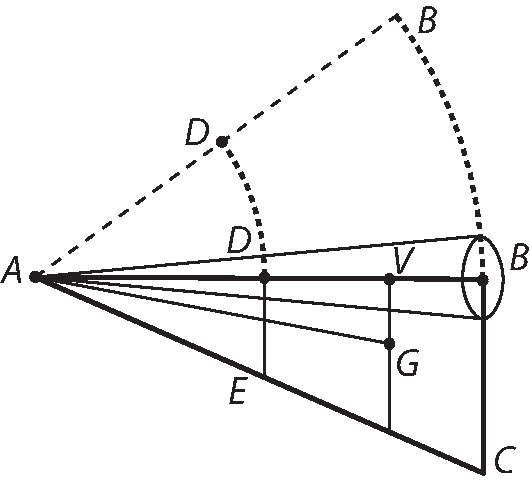
\includegraphics[trim = 0mm 0mm -4mm 0mm, clip, width=0.42\textwidth]{images/LH035,14,02_121r-d1.pdf}
\noindent
\centering
[\textit{Fig. 21}]\edtext{}{\lemma{\hspace*{1,8mm}[\textit{Fig. 21}]}\killnumber\Cfootnote{Vgl. \cite{00301}a.a.O., Fig. 307 (\cite{01008}\textit{WO} I, S. 1013).}}
\end{wrapfigure}
\noindent\edtext{%
Eadem si $\displaystyle AB$ intelligatur esse conus seu pyramis
erunt ejus particulae ab $\displaystyle A$ vertice numeratae 
crescentes ut 1. 4. 9. series
[secundanorum].\edtext{}{\lemma{primanorum}\Bfootnote{\textit{L ändert Hrsg. nach Vorlage}}}
Celeritates autem cujus\-libet puncti ut series primanorum:
\edtext{1. 2. 3. Ergo}{%
\lemma{}\Bfootnote{1. 2. 3.\ \textbar\ 4. \textit{gestr.}\ \textbar\ Ergo\ \textit{L}}}
momentum ut series tertianorum 1. 8. 27.
\edtext{unde trilineo parabolico cubicali applicato,
et ducta per ejus centrum gravitatis recta,}{%
\lemma{unde}\Bfootnote{%
\textit{(1)}\ si
\textit{(2)}\ trilineo [...] recta,
\textit{L}}}
\edtext{ea in axe dabit centrum aequilibrii.}{%
\lemma{ea}\Bfootnote{%
\textit{(1)}\ dabit centrum virium in pyram
\textit{(2)}\ in axe [...] aequilibrii.
\textit{L}}}}{%
\lemma{Eadem [...] aequilibrii}%
\Cfootnote{\cite{00301}a.a.O., S. 679 (\cite{01008}\textit{WO} I, S. 1014).\hspace{-4mm}}}
%
\edtext{Nempe generaliter componenda series ponderum\protect\index{Sachverzeichnis}{pondus}
cum serie celeritatum utcunque quaesita,\protect\index{Sachverzeichnis}{celeritas quaesita}
ut habeatur series virium, quae si
\edtext{considerentur ut librae\protect\index{Sachverzeichnis}{libra} gravamina,}{%
\lemma{considerentur ut}\Bfootnote{%
\textit{(1)}\ momenta
\textit{(2)}\ librae gravamina
\textit{L}}}
eisdem legibus hic exquiretur centrum gravitatis,\protect\index{Sachverzeichnis}{centrum gravitatis}
quibus supra centrum
aequilibrii}{%
\lemma{Nempe [...] aequilibrii}%
\Cfootnote{\cite{00301}a.a.O., S. 679f. (\cite{01008}\textit{WO} I, S. 1014).}}%
%
\edtext{. Non}{%
\lemma{aequilibrii.}\Bfootnote{%
\textit{(1)}\ Notandum
\textit{(2)}\ Non
\textit{L}}}
satis diserte explicat unum,
quae scilicet sit recta $\displaystyle AB$ ad quam fieri debet applicatio.
Unde vocat axem figurae
\edtext{ut Trianguli,}{%
\lemma{}\Bfootnote{ut\ \textbar\ lineae, \textit{gestr.}\ \textbar\ Trianguli,\ \textit{L}}}
pyramidis, coni, sed in his figuris,
quae similiter per medium dividi possunt,
facile patet axis.
Ac vero in aliis, erit $\displaystyle AB$ semper
\edtext{recta quae transit per ipsius figurae,
v.g. si sit semiconus, centrum gravitatis,
et simul per axem rotationis.}{%
\lemma{recta}\Bfootnote{%
\textit{(1)}\ quae transit per axem
\textit{(2)}\ quae [...] rotationis
\textit{L}}}
Ita puto, etsi diserte non dicat Wallisius.
\edlabel{LH35,14,02_121r_ref-5}Videtur tandem dicere, sed non demonstrat.\edlabel{LH35,14,02_121r_ref-6}
\pend
\pstart
\edtext{Quod si jam aliquis manu aliterve impediat rotationem,
res redibit ad superiora de duobus fulcris
(+~dubito, nam in duobus fulcris indeterminatum punctum rotationis, hic determinatur~+)
et loco supra centri gravitatis\protect\index{Sachverzeichnis}{centrum gravitatis}
substituendum nunc centrum percussionis.\protect\index{Sachverzeichnis}{centrum percussionis}}{%
\lemma{Quod [...] percussionis}%
\Cfootnote{\cite{00301}a.a.O., S. 680 (\cite{01008}\textit{WO} I, S. 1014).}}
%
\pend
\count\Afootins=1000
\count\Bfootins=1000
\count\Cfootins=1000
\pstart
Denique monet
\edtext{\textit{processum a dato corporis percutientis centro gravitatis ad ejusdem circa axem datum centrum virium} requirendum
% In der Vorlage \textit{inquirendum}
\textit{alium non esse quam a dato plani centro gravitatis ad ungulae eidem insistentis centrum gravitatis.}}{%
\lemma{\textit{processum} [...] \textit{gravitatis}}%
\Cfootnote{\cite{00301}a.a.O. (\cite{01008}\textit{WO} I, S. 1014f.). Zitat mit Auslassungen.\hspace{-4mm}}}
%
[121~v\textsuperscript{o}] %%%%%%%%%%  HIER BEGINNT BLATT 121v.
%
\edtext{%
\textit{Porro cum centrum virium\protect\index{Sachverzeichnis}{centrum virium}
sit ut plurimum saltem intra ipsum solidum,
percussio autem a solido facta sit in superficiei puncto aliquo;
si quis quaerat in quo superficiei puncto pro hoc aut illo solidi percutientis situ}
res \textit{contingat}, dicendum est
\textit{in eo superficiei puncto} id \textit{contingere}
(+~credo ut sit maxima percussio\protect\index{Sachverzeichnis}{percussio}~+),
\textit{quod est in} linea directionis \textit{centri virium,
in ictus\protect\index{Sachverzeichnis}{ictus} instanti.}}{%
\lemma{\textit{Porro} [...] \textit{instanti}}%
\Cfootnote{\cite{00301}a.a.O., S. 681 (\cite{01008}\textit{WO} I, S. 1015). Zitat mit Auslassungen.}}
%
Itaque \edtext{inquit \edtext{grave\protect\index{Sachverzeichnis}{grave} [si] percussionem spectes}{%
\lemma{grave}\Bfootnote{%
\textit{(1)}\ si ponderationem aestim
\textit{(2)}\ \textbar\ si \textit{erg. Hrsg.}\ \textbar\ percussionem spectes
\textit{L}}}
perinde se habere,
ac si totum sit in
\edtext{centro percussionis.}{%
\lemma{centro}\Bfootnote{%
\textit{(1)}\ gravitatis
\textit{(2)}\ percussionis
\textit{L}}}}{%
\lemma{inquit [...] percussionis}%
\Cfootnote{\cite{00301}a.a.O.\cite{01008}}}
%
Et \edtext{%
\textit{hinc} inquit
\textit{ad funependula\protect\index{Sachverzeichnis}{funependulum}
aestimanda via patet}[,]
\textit{nempe cujuscunque figurae sit suspensum solidum,
puta cylindricum, Conicum, aliudve,
tantae longitudinis}[,]
\textit{vibrationem\protect\index{Sachverzeichnis}{vibratio} quod spectat}[,]
\textit{reputandum esse
quanta est \edtext{distantia a puncto suspensionis}{%
\lemma{distantia a}\Bfootnote{%
\textit{(1)}\ vibrationis
\textit{(2)}\ \textit{puncto suspensionis}
\textit{L}}}
ad centrum virium.
Adeoque verbi gratia,
dato quod funependula ejusdem longitudinis aequalibus temporibus vibrent;
si conus vertice suspensus,
cujus centrum virium,\protect\index{Sachverzeichnis}{centrum virium}
ut ex calculo superius insinuato}[,]
\protect\rule[-4mm]{0mm}{10mm}\textit{a vertice distet $\displaystyle \frac{4}{5}$ totius altitudinis}[,]
\textit{cum globulo ex tenuissimo 
\edtext{filo (cujus consideratio itaque non habetur) suspenso,%
}{\lemma{filo}\Bfootnote{%
\textit{(1)}\ \textit{suspenso}
\textit{(2)}\ \textit{(cujus} [...] \textit{suspenso}
\textit{L}}}
cujus longitudo sit
(a puncto suspensionis ad centrum virium globuli)
% [...]
ut 4 ad 5. aequalibus temporibus vibrabitur uterque,}
\edtext{ob aequalem distantiam centri virium.\protect\index{Sachverzeichnis}{centrum virium}}{%
\lemma{ob [...] virium}%
\Cfootnote{In der Vorlage \textit{utpote quorum Centrum virium aequaliter a puncto suspensionis distant.}}}%
}{%
\lemma{\textit{hinc} [...] virium}%
\Cfootnote{\cite{00301}a.a.O., S. 681f. (\cite{01008}\textit{WO} I, S. 1015). Zitat mit Auslassungen.}}
%
\pend
\vspace{2.5em}
\count\Afootins=1500
\count\Bfootins=1500
\count\Cfootins=1500
\pstart
\noindent\centering
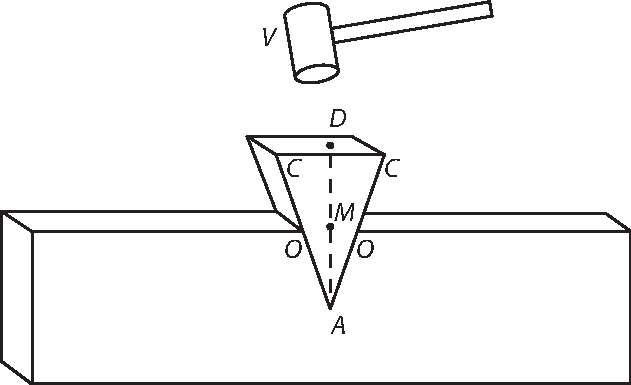
\includegraphics[width=0.7\textwidth]{images/LH035,14,02_121v-d1.pdf}\\%
\vspace*{0.2em}%
[\textit{Fig. 22}]\edtext{}{\lemma{\hspace*{1,8mm}[\textit{Fig. 22}]}\killnumber\Cfootnote{Vgl. \cite{00301}a.a.O., pars III, cap. 12, Fig. 309 (\cite{01008}\textit{WO} I, S. 1016).}}
\pend
\newpage
%\vspace*{1.5em}% PR: Rein provisorisch !!!!
\pstart
Cap. XII. de Cuneo.
Non contemnendum videtur quod de eo habet paucis:
\edtext{%
\textit{intelligatur} inquit \textit{ligni tenacitas
seu firmitudo cuneo\protect\index{Sachverzeichnis}{cuneus} divellenda,}
vel \textit{quorumvis obicum\protect\index{Sachverzeichnis}{obex}
cuneo divellendorum resistentia\protect\index{Sachverzeichnis}{resistentia} ut $\displaystyle O.$}
[\textit{Dico}]\edtext{}{\lemma{Dic}\Bfootnote{\textit{L ändert Hrsg. nach Vorlage}}}
\textit{primo: si adhibeatur in cunei dorso $\displaystyle D.$
vis $\displaystyle V$ quae sit ad $\displaystyle O,$
ut $\displaystyle CC$ cunei crassities ad ejusdem altitudinem $\displaystyle DA,$}
seu \textit{ut} [$\displaystyle c$]\edtext{}{\lemma{$\displaystyle C$}\Bfootnote{\textit{L ändert Hrsg. nach Vorlage}}}
\textit{ad} [$\displaystyle a.$]\edtext{}{\lemma{$\displaystyle A.$}\Bfootnote{\textit{L ändert Hrsg. nach Vorlage}}}
\textit{vis illa in $\displaystyle D$ aequipollebit obici,
adeoque aucta superabit.
Nam cum per \edtext{prop. 5. cap. 2.}{%
\lemma{prop. 5. cap. 2 }%
\Cfootnote{\cite{00301}a.a.O., pars I, S. 37f. (\cite{01008}\textit{WO} I, S. 597).}}
motus in ea ratione polleant,
quae ex rationibus virium motricium\protect\index{Sachverzeichnis}{vis motrix}
et progressuum regressuumve secundum lineam directionis suae componitur,
sitque amolitio obicis}[,]\protect\index{Sachverzeichnis}{obex}
\textit{contra directionem suam,
ad progressum virium
(secundum directionem suam}[\textit{)}]\edtext{}{\lemma{\textit{)}}\Bfootnote{\textit{erg. Hrsg. nach Vorlage}}}
\textit{\edtext{ut $\displaystyle c$ ad $\displaystyle a$}{%
\lemma{ut}\Bfootnote{%
\textit{(1)}\ $\displaystyle C$ \textit{ad} $\displaystyle A$
\textit{(2)}\ $\displaystyle c$ \textit{ad} $\displaystyle a$
\textit{L}}}
seu $\displaystyle CC$ ad $\displaystyle DA,$}
quia \textit{dum detruditur cuneus per totam altitudinem,
dirimitur obex per totam crassitiem,
et in toto processu proportionaliter.}
Ideo \textit{si vires $\displaystyle V.$ $\displaystyle O$ sint
ipsis $\displaystyle a.$ $\displaystyle c$ progressibus suis
reciproce proportionales aequipollebunt motus},
quia ratio ex reciprocis composita est aequalitatis.
Si jam mallei\protect\index{Sachverzeichnis}{malleus} vis composita\protect\index{Sachverzeichnis}{vis composita}
ex ejus pondere\protect\index{Sachverzeichnis}{pondus} et celeritate,\protect\index{Sachverzeichnis}{celeritas}
\protect\rule[-4mm]{0mm}{10mm}seu $\displaystyle PC\, \sqcap\, V\, \sqcap \edtext{\frac{c}{a}O$ cuneo}{%
\lemma{$\displaystyle \frac{c}{a}O$}\Bfootnote{%
\textit{(1)}\ malleo
\textit{(2)}\ cuneo
\textit{L}}}
directe applicata[,]%
[obici]\edtext{}{\lemma{obici}\Bfootnote{\textit{erg. Hrsg. nach Vorlage}}}
aequipollebit.
Idem ait esse de celeritate
\edtext{quaesita. \textit{Et}}{%
\lemma{quaesita.}\Bfootnote{%
\textit{(1)}\ Ergo
\textit{(2)}\ \textit{Et}
\textit{L}}}
\textit{quidem ob eandem causam eousque amovere seu amoliri perseverabit
donec sic impensa vis, $\displaystyle PC$
particulis cuneo\protect\index{Sachverzeichnis}{cuneus} propioribus rumpendis aut flectendis
per \edtext{aequipollentiam absorbeatur.}{%
\lemma{aequipollentiam}\Bfootnote{%
\textit{(1)}\ impendatur,
\textit{(2)}\ \textit{absorbeatur.}
\textit{L}}}
Idemque momentum secundo adhibitum tantundem praestabit, et tertio tantundem},
et ita porro.}{%
\lemma{\textit{intelligatur} [...] porro}%
\Cfootnote{\cite{00301}a.a.O., prop. 1, S. 684 (\cite{01008}\textit{WO} I, S. 1016f.).}}
%
\pend
\count\Afootins=1200
\count\Bfootins=1200
\count\Cfootins=1200
\pstart
\edtext{Scholium,
\textit{sunt qui cuneum ad geminum vectem\protect\index{Sachverzeichnis}{vectis} referunt
quibus vis in $\displaystyle CC$ applicetur,
fulcra\protect\index{Sachverzeichnis}{fulcrum} autem alii in $\displaystyle OO$ ponunt,
oneraque\protect\index{Sachverzeichnis}{onus} in $\displaystyle A$ utrinque protrudenda.
Alii potius fulcrum commune in $\displaystyle A$ ponunt,
et onera\protect\index{Sachverzeichnis}{onus} in $\displaystyle OO$
(eo potissimum, quod in lignis\protect\index{Sachverzeichnis}{lignum} aliisque diffindendis cunei acies non semper rem diffindendam}
[\textit{attingit}]\edtext{}{\lemma{\textit{attingit}}\Bfootnote{\textit{erg. Hrsg. nach Vorlage}}}
\textit{uspiam sed medio suspensa} manet,
\textit{adeoque dici non potest} pondus\protect\index{Sachverzeichnis}{pondus} \textit{depelleret.}%
[\textit{)}]\edtext{}{\lemma{\textit{)}}\Bfootnote{\textit{erg. Hrsg. nach Vorlage}}}
\textit{Ego vero ut alia incommoda taceam
rem simplicius exponendam duxi ex ipsis motuum elementis.}}{%
\lemma{Scholium [...] \textit{elementis}}%
\Cfootnote{\cite{00301}a.a.O., pars III, cap. 12, prop. 1, S. 685 (\cite{01008}\textit{WO} I, S. 1017). Zitat mit Auslassungen.}}
%
\pend
\pstart
\edtext{Addit \textit{eadem similiter accommodari posse,
Malleo\protect\index{Sachverzeichnis}{malleus} ferreo clavum\protect\index{Sachverzeichnis}{clavus} adigenti,
Tuditi\protect\index{Sachverzeichnis}{tudes} praegrandi}
\protect\index{Sachverzeichnis}{pilum}[\textit{pila}],\edtext{}{\lemma{pilae}\Bfootnote{\textit{L ändert Hrsg. nach Vorlage}}}
\textit{sudes\protect\index{Sachverzeichnis}{sudes} palosve\protect\index{Sachverzeichnis}{palus}}
\edtext{praegrandes}{\lemma{praegrandes}\Cfootnote{In der Vorlage \textit{praeacutos}.}}
\textit{in terram infigenti altius:}
Nam hi \textit{cunei\protect\index{Sachverzeichnis}{cuneus} sunt qui malleo adiguntur:}
In \textit{ascia,\protect\index{Sachverzeichnis}{ascia} bipenni,\protect\index{Sachverzeichnis}{bipennis}
\edtext{securi,\protect\index{Sachverzeichnis}{securis} malleus}{%
\lemma{securi,}\Bfootnote{%
\textit{(1)}\ acies
\textit{(2)}\ malleus
\textit{L}}}
cuneo connexus} est.}{%
\lemma{Addit [...] \textit{connexus} est}%
\Cfootnote{\cite{00301}a.a.O., prop. 2, S. 685 (\cite{01008}\textit{WO} I, S. 1017). Zitat mit Auslassungen.}}
%
Haec ille.
\pend
\pstart
Ego difficultates quasdam reperio.
Nam si tantum pondus consideretur separandorum 
vel ponatur appensum pondus,
quod ea contineat, verum erit, quod dicit.
Sed sciendum abstrahendo a pondere\protect\index{Sachverzeichnis}{pondus}
si difficultas sit tantum in ipsa separatione seu glutine,\protect\index{Sachverzeichnis}{gluten}
tunc primum momentum\protect\index{Sachverzeichnis}{momentum} aestimandum,
quanta scilicet \edtext{celeritate\protect\index{Sachverzeichnis}{celeritas} divellatur,}{%
\lemma{celeritate}\Bfootnote{%
\textit{(1)}\ debeat
\textit{(2)}\ divellatur
\textit{L}}}
seu quanti cunei introitu.
Imo videtur res redire ad
Wallisii\protect\index{Namensregister}{\textso{Wallis} (Wallisius), John 1616-1703}
regulam ponendo $\displaystyle AO$ quae introiit, infinite parvam
ut et $\displaystyle OO$ divulsionem.
Nempe si cuneus\protect\index{Sachverzeichnis}{cuneus} sit instar Trianguli
ponendo $\displaystyle M$ punctum medium
\edtext{ipsius $\displaystyle OO$ tunc $\displaystyle MA,$ ducenda in vim applicatam;\protect\index{Sachverzeichnis}{vis applicata} $\displaystyle MO$ in resistentiam,\protect\index{Sachverzeichnis}{resistentia}
ut intelligatur utriusque vis, in se invicem.}{%
\lemma{ipsius $\displaystyle OO$}\Bfootnote{%
\textit{(1)}\ faciendum, ut $\displaystyle MA$ ad $\displaystyle MO$ ita est
\textit{(2)}\ tunc [...] invicem.
\textit{L}}}
\pend
\count\Afootins=1000
\count\Bfootins=1000
\count\Cfootins=1000
% \newpage% PR: Rein provisorisch !!!
\vspace{1em}
\pstart
\edtext{Sequitur Cap. XIII. de Elatere\protect\index{Sachverzeichnis}{elater} \pgrk{>elat'hr.}
Vis \pgrk{>elastik'h}, ab \pgrk{>ela'unw,} abigo excutio expello.}{%
\lemma{Sequitur [...] expello}%
\Cfootnote{\cite{00301}a.a.O., cap. 13, S. 686 (\cite{01008}\textit{WO} I, S. 1018).}}
Propositiones suas deducit ex ictus magnitudine:\protect\index{Sachverzeichnis}{ictus}
Nempe:
\edtext{\textit{Si grave\protect\index{Sachverzeichnis}{grave} motum
in firmum obicem\protect\index{Sachverzeichnis}{obex} directe impingat,
sitque vel alterum vel utrumque corpus Elasticum,\protect\index{Sachverzeichnis}{corpus elasticum}
eadem celeritate\protect\index{Sachverzeichnis}{celeritas} resiliet seu repercutietur, qua advenerat,
et per eandem rectam.}}{%
\lemma{\textit{Si grave} [...] \textit{rectam}}%
\Cfootnote{\cite{00301}a.a.O., prop. 1, S. 687 (\cite{01008}\textit{WO} I, S. 1018).}}
%
\pend
\pstart
\edtext{\textit{Si grave motum in firmum obicem oblique impingat,
sitque vel alterum, vel utrumque elasticum}[,]
\textit{resilitio\protect\index{Sachverzeichnis}{resilitio} eadem celeritate et in eodem plano ita fiet,}
ut sint anguli incidentiae\protect\index{Sachverzeichnis}{incidentia}
angulis reflexionis\protect\index{Sachverzeichnis}{reflexio} aequales.}{%
\lemma{\textit{Si grave} [...] aequales}%
\Cfootnote{\cite{00301}a.a.O., prop. 2, S. 692 (\cite{01008}\textit{WO} I, S. 1021).\hspace{-3mm}}}
%
\edtext{Hoc recte demonstrat.}{%
\lemma{Hoc [...] demonstrat}%
\Cfootnote{\cite{00301}a.a.O.\cite{01008}}}
\pend
\pstart
\edtext{\textit{Si duo gravia invicem aequalia aequali celeritate sibi mutuo directe occurrant,
sintque alterum, vel utrumque corpora Elastica,}
%
[122~r\textsuperscript{o}] %%%%%%%%%%  HIER BEGINNT BLATT 122r.
%
\textit{aut etiam si gravia\protect\index{Sachverzeichnis}{grave} illa sint inaequalia
sed celeritates\protect\index{Sachverzeichnis}{celeritas} habeant reciproce proportionales
(quo saltem momenta sint aequalia):
Resiliet utrumque eadem celeritate
qua accesserat, et per eandem rectam.}}{%
\lemma{\textit{Si duo} [...] \textit{rectam}}%
\Cfootnote{\cite{00301}a.a.O., prop. 3, S. 695 (\cite{01008}\textit{WO} I, S. 1023).}}%
%
\edtext{ \\%
\hspace*{7,5mm}%
Si\edlabel{35,14,02_122r_1}\edtext{}{{%
\xxref{35,14,02_122r_1}{35,14,02_122r_2}}
\lemma{Si motis [...] de ictu}%
\Cfootnote{\cite{00301}a.a.O., prop. 4, S. 696f. (\cite{01008}\textit{WO} I, S. 1024). Siehe \cite{00301}a.a.O., cap. 11, prop. 8, S. 669 (\cite{01008}\textit{WO} I, S. 1007).}}
motis communis addatur}{%
\lemma{\textit{rectam.}}\Bfootnote{%
\textit{(1)}\ Si gravibus motis communis add
\textit{(2)}\ Si [...] addatur
\textit{L}}}
celeritas vel auferatur,
perinde omnia eveniunt,
quoad impulsum\protect\index{Sachverzeichnis}{impulsus} vel Elateris\protect\index{Sachverzeichnis}{elater}
\edtext{compressionem, (ut supra de ictu).\edlabel{35,14,02_122r_2}\\%
\hspace*{7,5mm}\textit{Si} }{\lemma{compressionem}\Bfootnote{%
\textit{(1)}\ . \textit{Si gra}
\textit{(2)}\ , (ut supra [...] \textit{Si grave}
\textit{L}}}\edtext{%
\textit{grave motum aequali quiescenti}[,]
non \textit{impedito tamen}[,]
\textit{directe impingat,
sitque vel alterum vel utrumque Elasticum,
motum quiescet, et quiescens movebitur ea celeritate quae}
[\textit{fuerat}]\edtext{}{\lemma{fuerant}\Bfootnote{\textit{L ändert Hrsg. nach Vorlage}}}
\textit{prius moti.}}{%
\lemma{\textit{Si grave} [...] \textit{moti}}%
\Cfootnote{\cite{00301}a.a.O., cap. 13, prop. 5, S. 697 (\cite{01008}\textit{WO} I, S. 1025).}}
%
Congerit ejus propositionis quatuor vel saltem tres demonstrationes.
Quas describere operae pretium erit:
\pend
\count\Afootins=1200
\count\Bfootins=1200
\count\Cfootins=1200
\pstart
\edtext{\textit{Esto gravium hujusmodi invicem aequalium $\displaystyle A.\, B$
pondus\protect\index{Sachverzeichnis}{pondus} utriusvis}
[$\displaystyle mP$]\edtext{.}{\lemma{$\displaystyle MP$}\Bfootnote{\textit{L ändert Hrsg. nach Vorlage}}}
\textit{Quorum $\displaystyle B$ quiescat,
eique directe impingat $\displaystyle A$ celeritate $\displaystyle rC.$
adeoque momento\protect\index{Sachverzeichnis}{momentum} seu impetu\protect\index{Sachverzeichnis}{impetus} $\displaystyle mrPC\ \sqcap\ mP \smallfrown rC.$
Vim\protect\index{Sachverzeichnis}{vis} huic aequipollentem imprimeret Elateri,
eadem seipsum exuens}[;]
\textit{qua (retenta) Elater post repelleret ipsum $\displaystyle A$
(ad quietem redactum)}[,]
\textit{modo $\displaystyle B$ firmum esset,
per \edtext{prop. 1 hujus}{%
\lemma{prop. 1 hujus}%
\Cfootnote{\cite{00301}a.a.O., S. 687 (\cite{01008}\textit{WO} I, S. 1018).\hspace{25mm}}}
(ut taceam id quod est ab obice\protect\index{Sachverzeichnis}{obex} et in obicem rependitur).
Sed propter non impediti $\displaystyle B$ cessionem,
quam ab $\displaystyle A$ recipit vim Elater,\protect\index{Sachverzeichnis}{elater}
eandem cedenti $\displaystyle B$ protinus impertit
(nec in se retinet, ut in casu prop. 1. quo possit $\displaystyle A$ post repellere.)
Unde factum}
[\textit{est}]\edtext{}{\lemma{\textit{est}}\Bfootnote{\textit{erg. Hrsg. nach Vorlage}}}
\textit{ut impellens $\displaystyle A$
(vi sua destitutum, quam in Elaterem impenderat)
quiescat; eaque vi $\displaystyle mrPC$ elateris interventu in $\displaystyle B$ collata,
propellatur $\displaystyle B.$ adeoque (propter}
[$\displaystyle mP$]\edtext{}{\lemma{$\displaystyle MP$}\Bfootnote{\textit{L ändert Hrsg. nach Vorlage}}}
\textit{pondus) celeritate $\displaystyle rC$ (prorsum) quae fuerat impellentis.}}{%
\lemma{\textit{Esto} [...] \textit{impellentis}}%
\Cfootnote{\cite{00301}a.a.O., S. 697f. (\cite{01008}\textit{WO} I, S. 1025).}}
%
\pend
\count\Afootins=1200
\count\Bfootins=1200
\count\Cfootins=1200
\pstart
\edtext{\textit{\textso{Demonstratio alia.}
Sunto hujusmodi gravia\protect\index{Sachverzeichnis}{grave} aequalia $\displaystyle A.\, B$
quorum utrius\-vis pondus\protect\index{Sachverzeichnis}{pondus}
\edtext{sit $\displaystyle mP$}{%
\lemma{sit}\Bfootnote{%
\textit{(1)}\ $\displaystyle MP.$
\textit{(2)}\ $\displaystyle mP.$
\textit{L}}}
atque in $\displaystyle B$ quiescens directe impingat $\displaystyle A$, celeritate $\displaystyle rC$,
\edtext{adeoque momento\protect\index{Sachverzeichnis}{momentum}}{%
\lemma{adeoque}\Bfootnote{%
\textit{(1)}\ celeritate
\textit{(2)}\ \textit{momento}
\textit{L}}}
seu impetu $\displaystyle mrPC.$
Quo itaque propter cessionem non impediti $\displaystyle B$
utraque junctim ferenda essent,
(si vis Elastica\protect\index{Sachverzeichnis}{vis elastica} abesset)
celeritate\protect\index{Sachverzeichnis}{celeritas} dimidia \protect\rule[-4mm]{0mm}{10mm}$\displaystyle\frac{1}{2}rC$ prorsum
(propter $\displaystyle \protect\rule[-4mm]{0mm}{10mm}mrPC\ \sqcap\ 2mP \smallfrown \frac{1}{2}rC$}%
[\textit{)}]\edtext{}{\lemma{\textit{)}}\Bfootnote{\textit{erg. Hrsg. nach Vorlage}}}
propter \edtext{\textit{prop. 2}}{%
\lemma{\textit{prop. 2}}%
\Cfootnote{\cite{00301}a.a.O., cap. 11, S. 662f. (\cite{01008}\textit{WO} I, S. 1003f.).}}
cap. 11.
\textit{Sed (propter vim Elasticam,) Elateri imprimitur vis restitutiva,\protect\index{Sachverzeichnis}{vis restitutiva}
ipsi $\displaystyle mrPC$ aequipollens
(nam quamdiu}
[\textit{Elateris}]\edtext{}{\lemma{Elaterius}\Bfootnote{\textit{L ändert Hrsg. nach Vorlage}}}
\textit{flexio\protect\index{Sachverzeichnis}{flexio} facilius fiat,
quam utriusque gravis\protect\index{Sachverzeichnis}{grave} processus,
Elater\protect\index{Sachverzeichnis}{Elater} porro flectitur,
et qua vi flectitur,
eadem propter vim Elasticam\protect\index{Sachverzeichnis}{vis elastica} se restituit).
Elater\protect\index{Sachverzeichnis}{Elater} itaque utrinque se explicare satagens,
(diremtis invicem gravibus)
repellit $\displaystyle A$, \protect\rule[-4mm]{0mm}{10mm}vi $\displaystyle\frac{1}{2}mrPC$
\edtext{atque eadem vi}{\lemma{atque eadem vi}\Bfootnote{\textit{erg. L}}}
propellit $\displaystyle B.$
adeoque (propter pondus utrobique
\edtext{$\displaystyle mP$) A quidem celeritate}{%
\lemma{$\displaystyle mP$)}\Bfootnote{%
\textit{(1)}\ atque ideo propter
\textit{(2)}\ \textit{A quidem celeritate}
\textit{L}}}
\protect\rule[-4mm]{0mm}{10mm}$\displaystyle -\frac{1}{2}rC$ retrorsum,
$\displaystyle B$ vero celeritate $\displaystyle +rC$ prorsum}
(legendum $\displaystyle +\frac{1}{2}rC$ prorsum).
\textit{Sed ferendum erat $\displaystyle A$ alio nomine}[,]
\textit{ut dictum est}[,]
\textit{celeritate $\displaystyle +rC$}
(+~legendum \protect\rule[-4mm]{0mm}{10mm}$\displaystyle +\frac{1}{2}rC$~+)
\textit{prorsum.
Ergo cum hoc nomine accedat celeritas $\displaystyle -rC$ retrorsum}
(+~lege $\displaystyle -\frac{1}{2}rC$ retrorsum~+)
\textit{quiescet $\displaystyle A.$}
At $\displaystyle B$ ferendum ob Elaterem\protect\index{Sachverzeichnis}{elater} celeritate \protect\rule[-4mm]{0mm}{10mm}$\displaystyle +\frac{1}{2}rC$
et alio nomine etiam \protect\rule[-4mm]{0mm}{10mm}$\displaystyle +\frac{1}{2}rC.$
unde feretur celeritate\protect\index{Sachverzeichnis}{celeritas} $\displaystyle +rC,$
nempe \textit{prorsum,
hoc est quae fuerat prius moti, $\displaystyle A.$}}{%
\lemma{\textit{\textso{Demonstratio}} [...] \textit{moti, $\displaystyle A$}}%
\Cfootnote{\cite{00301}a.a.O., S. 698 (\cite{01008}\textit{WO} I, S. 1025).}}
%
\pend
\count\Afootins=1200
\count\Bfootins=1200
\count\Cfootins=1200
\pstart
\edtext{%
\textit{\textso{Vel sic brevius:}
Positis ut prius; ferenda essent utraque,
si Elater nullus foret,
celeritate \protect\rule[-4mm]{0mm}{10mm}$\displaystyle \frac{1}{2}rC$ prorsum
adeoque utrumvis}
(lege utriusvis)
\textit{momento seu vi \protect\rule[-4mm]{0mm}{10mm}$\displaystyle \frac{1}{2}mrPC$ 
per \edtext{prop. 2}{%
\lemma{prop. 2}%
\Cfootnote{\cite{00301}a.a.O., cap. 11, S. 662f. (\cite{01008}\textit{WO} I, S. 1003f.).}}
cap. 11.
Est autem per \edtext{prop. 9}{%
\lemma{prop. 9}%
\Cfootnote{\cite{00301}a.a.O., S. 670 (\cite{01008}\textit{WO} I, S. 1008).}}
cap. 11
ictus \protect\index{Sachverzeichnis}{ictus} magnitudo $\displaystyle mrPC$
atque huic aequalis vis Elateris\protect\index{Sachverzeichnis}{vis elateris} restitutiva\protect\index{Sachverzeichnis}{vis restitutiva}
per \edtext{demonstrata ad prop. 1.}{%
\lemma{demonstrata ad prop. 1.}%
\Cfootnote{\cite{00301}a.a.O., cap. 13, S. 687-690 (\cite{01008}\textit{WO} I, S. 1018-1020).}}
quae se utrinque explicare satagens
dimidia vi tum repellit $\displaystyle A.$ tum propellit $\displaystyle B.$
adeoque ipsi $\displaystyle A$ impertit vim \protect\rule[-4mm]{0mm}{10mm}$\displaystyle -\frac{1}{2}mrPC$ (retrorsum),
et $\displaystyle B$ vim $\displaystyle \frac{1}{2}mrPC$ (prorsum)
quae si prius positis respective addantur,
fiet vis in $\displaystyle A$
\protect\rule[-4mm]{0mm}{10mm}$\displaystyle \sqcap\ \frac{1}{2}mrPC - \frac{1}{2}mrPC\ \sqcap\ 0PC.$}
ergo \textit{quiescet,
in $\displaystyle B$ vero \protect\rule[-4mm]{0mm}{10mm}$\displaystyle \sqcap\ \frac{1}{2}mrPC + \frac{1}{2}mrPC\ \sqcap\ mrPC.$
quod itaque propter pondus $\displaystyle mP,$
feretur prorsum celeritate $\displaystyle rC$
quae fuerat ipsius $\displaystyle A.$}}{%
\lemma{\textit{\textso{Vel sic}} [...] \textit{ipsius $\displaystyle A$}}%
\Cfootnote{\cite{00301}a.a.O., cap. 13, S. 698f. (\cite{01008}\textit{WO} I, S. 1025). Zitat mit Auslassung.}}
%
\pend
\pstart
\edtext{\textit{\textso{Adhuc alia:}
Sunto ea gravia\protect\index{Sachverzeichnis}{grave} aequalia,
ut prius $\displaystyle A.$ $\displaystyle B.$
et quiescenti $\displaystyle B$ directe impingat $\displaystyle A$
celeritate\protect\index{Sachverzeichnis}{celeritas} $\displaystyle rC$ prorsum.
Intelligatur autem utrique superaddi motus communis,
celeritate \protect\rule[-4mm]{0mm}{10mm}$\displaystyle -\frac{1}{2}rC$ retrorsum,
quo fiat gravis $\displaystyle A$ celeritas \protect\rule[-4mm]{0mm}{10mm}$\displaystyle rC - \frac{1}{2}rC$ prorsum,
et gravis B celeritas $\displaystyle -\frac{1}{2}rC$ retrorsum.}
\edtext{[\textit{Quo casu, ferretur $\displaystyle A$
post contactum\protect\index{Sachverzeichnis}{contactus}
celeritate $\displaystyle -\frac{1}{2}rC$ (retrorsum),}]}{%
\lemma{\textit{Quo casu} [...] \textit{(retrorsum),}}\Bfootnote{\textit{erg. Hrsg. nach Vorlage}}}
\textit{et $\displaystyle B$ celeritate $\displaystyle \frac{1}{2}rC$ prorsum
per \edtext{prop. 3. hujus.}{%
\lemma{prop. 3. hujus}%
\Cfootnote{\cite{00301}a.a.O., S. 695f. (\cite{01008}\textit{WO} I, S. 1023).}}
Sed propter communem motum}
qui hic est nullius instar quoad impulsum,\protect\index{Sachverzeichnis}{impulsus}
\edtext{prop. praeced.}{%
\lemma{prop. praeced.}%
\Cfootnote{\cite{00301}a.a.O., prop. 4, S. 696 (\cite{01008}\textit{WO} I, S. 1024).}}
\textit{idem erit effectus\protect\index{Sachverzeichnis}{effectus} impulsus in casu praesenti.
Si itaque in statum pristinum restituantur demta utrinque quae addebatur celeritate \protect\rule[-4mm]{0mm}{10mm}$\displaystyle -\frac{1}{2}rC$
seu}[,] \textit{quod \edtext{eodem recidit}{%
\lemma{eodem}\Bfootnote{%
\textit{(1)}\ redidit
\textit{(2)}\ \textit{recidit}
\textit{L}}}}[,]
\textit{addita celeritate
\edtext{$\displaystyle +\frac{1}{2}rC$}{%
\lemma{$\displaystyle +\frac{1}{2}rC$}%
\Cfootnote{In der Vorlage $\displaystyle +rC.$}}
prorsum. Habebitur gravis\protect\index{Sachverzeichnis}{grave} $\displaystyle A$
celeritas $\displaystyle -\frac{1}{2}rC +\frac{1}{2}rC\, \sqcap\, 0C.$
et gravis}
[$\displaystyle B$]\edtext{}{\lemma{$\displaystyle B$}\Bfootnote{\textit{erg. Hrsg. nach Vorlage}}}
\textit{celeritas\protect\index{Sachverzeichnis}{celeritas} $\displaystyle +\frac{1}{2}rC +\frac{1}{2}rC\, \sqcap\, rC.$}}{%
\lemma{\textit{\textso{Adhuc}} [...] $\displaystyle\, \sqcap\ rC$}%
\Cfootnote{\cite{00301}a.a.O., S. 699 (\cite{01008}\textit{WO} I, S. 1025f.). Zitat mit Auslassung.}}
%
\pend
\vspace{0.4mm}
\count\Afootins=1200
\count\Bfootins=1200
\count\Cfootins=1200
\pstart
\edtext{Ex his quatuor demonstrationibus inquit
Wallisius\protect\index{Namensregister}{\textso{Wallis} (Wallisius), John 1616-1703}
\textit{prima} et \textit{secunda physicam rei causam\protect\index{Sachverzeichnis}{causa physica} magis explicant:
Penultima quae ex vi quae foret si Elater\protect\index{Sachverzeichnis}{elater} nullus esset,
eaque quae ex Elateris vi restitutiva\protect\index{Sachverzeichnis}{vis restitutiva}
ictui\protect\index{Sachverzeichnis}{ictus} semper aequali colligit vim integram,
meis hypothesibus cap. 11 traditis maxime accommoda est
et demonstratio Geometrica ut mihi videtur maxime genuina.
Adjunxi \edtext{tamen ultimam in eorum praesertim gratiam,}{%
\lemma{tamen}\Bfootnote{%
\textit{(1)}\ \textit{gratiam}
\textit{(2)}\ \textit{ultimam} [...] \textit{gratiam}
\textit{L}}}
\edtext{qui}{\lemma{qui}\Cfootnote{In der Vorlage (irrtümlich) \textit{quae}.}}
hypothesibus meis} nondum
\textit{\edtext{receptis, difficilius}{%
\lemma{receptis,}\Bfootnote{%
\textit{(1)}\ minus
\textit{(2)}\ \textit{difficilius}
\textit{L}}}}
fortasse \textit{sunt assensuri.
Ea quippe methodo,
quam una cum praecedente}[,]
\textit{sequentibus item propositionibus accommodo,
missis aliis ex solis prop 3 et 4 hujus admissis}
(+~\edtext{nempe
\edtext{prop. 3}{%
\lemma{prop. 3}%
\Cfootnote{\cite{00301}a.a.O., S. 695f. (\cite{01008}\textit{WO} I, S. 1023f.).}}
si celeritates\protect\index{Sachverzeichnis}{celeritas} reciproce proportionales ponderibus[,]\protect\index{Sachverzeichnis}{pondus}}{%
\lemma{nempe}\Bfootnote{%
\textit{(1)}\ si
\textit{(a)}\ gravitate\protect\index{Sachverzeichnis}{gravitas}
\textit{(b)}\ gravia\protect\index{Sachverzeichnis}{grave}
\textit{(2)}\ prop. 3
\textit{L}}}
resilire utrumque eadem vi qua accesserat et per eandem rectam,
et \edtext{prop. 4.}{%
\lemma{prop. 4}%
\Cfootnote{\cite{00301}a.a.O., S. 696f. (\cite{01008}\textit{WO} I, S. 1024).}}
de \edtext{additione motus%
}{\lemma{additione}\Bfootnote{%
\textit{(1)}\ impulsus\protect\index{Sachverzeichnis}{impulsus}
\textit{(2)}\ motus
\textit{L}}}
communis $\displaystyle mC$ mutante~+)
\textit{quas alii postulant potius quam probant, tamquam per se claras,
aut experimentis\protect\index{Sachverzeichnis}{experimentum} satis comprobatas,
sequentes solo calculo\protect\index{Sachverzeichnis}{calculus} elicit.}
Itaque \textit{non aliter ex meis hypothesibus\protect\index{Sachverzeichnis}{hypothesis}} pendent,
\textit{quam quod ego inde probo}
[\textit{propositionem}]\edtext{}{\lemma{\textit{propositionem}}\Bfootnote{\textit{erg. Hrsg. nach Vorlage}}}
\textit{tertiam hujus}
(+~\edtext{ut et Mariottus\protect\index{Namensregister}{\textso{Mariotte}, Edme, Seigneur de Chazeuil ca. 1620-1684}}{
\lemma{ut et Mariottus}%
\Cfootnote{\cite{00311}E. \textsc{Mariotte}, \textit{De la percussion}, Paris 1673, S. 42-44.}}~+)
%
[122~v\textsuperscript{o}] %%%%%%%%%%  HIER BEGINNT BLATT 122v.
%
\textit{quam alii gratis postulant.}}{%
\lemma{Ex his [...] \textit{postulant}}%
\Cfootnote{\cite{00301}a.a.O., S. 699f. (\cite{01008}\textit{WO} I, S. 1026). Zitat mit Auslassungen.}}
\edtext{Nostra Motuum phaenomena\protect\index{Sachverzeichnis}{phaenomenon}
prius fuere Societati Regiae\protect\index{Sachverzeichnis}{Royal Society} exhibita
et Regestis inserta quam aliorum
[Hypotheses]\edtext{}{\lemma{Hypotheses}\Bfootnote{\textit{erg. Hrsg. nach Vorlage}}}
vel vulgatae vel exhibitae,
consentiunt tamen cum phaenomenis\protect\index{Sachverzeichnis}{phaenomenon} Hypothesium\protect\index{Sachverzeichnis}{hypothesis}
Wrenni\protect\index{Namensregister}{\textso{Wren} (Wrennus), Christopher 1632-1723}
et Hugenii.\protect\index{Namensregister}{\textso{Huygens} (Hugenius, Ugenius, Hugens, Huguens), Christiaan 1629-1695}}{%
\lemma{Nostra [...] Hugenii}%
\Cfootnote{\cite{00301}J. \textsc{Wallis}, \textit{Mechanica}, pars III, cap. 13, London 1670-1671, S. 700 (\cite{01008}\textit{WO} I, S. 1026).
Siehe \textit{PT} 3 (1668), S. 864-866\cite{01065} und S. 867f.\cite{01066}
sowie \textit{PT} 4 (1669), S. 925-928.\cite{01067}}}
%
\pend
\pstart
Superest ut excerpam reliquas propositiones. 
\edtext{6.}{\lemma{6.}\Bfootnote{\textit{erg. L}}}
\edtext{\textit{Si duo gravia Elastica\protect\index{Sachverzeichnis}{grave elasticum}
invicem aequalia ferantur per eandem rectam ad easdem partes
celeritatibus\protect\index{Sachverzeichnis}{celeritas} inaequalibus,
et consequens majori celeritate latum antecedenti directe impingat,
ferentur post contactum\protect\index{Sachverzeichnis}{contactus} ad easdem partes
utraque celeritatibus alternatis seu invicem permutatis.}}{%
\lemma{\textit{Si duo} [...] \textit{permutatis}}%
\Cfootnote{\cite{00301}J. \textsc{Wallis}, \textit{Mechanica}, pars III, cap. 13, London 1670-1671, S. 700 (\cite{01008}\textit{WO} I, S. 1026).}} 
%
\pend
\pstart
\edtext{%
(7)}{\lemma{(7)}\Bfootnote{\textit{erg. L}}}
\edtext{\textit{Sin ad contrarias partes,
ferentur} et \textit{deinceps ad contrarias partes
\edtext{celeritatibus invicem}{%
\lemma{celeritatibus}\Bfootnote{%
\textit{(1)}\ iisdem
\textit{(2)}\ \textit{invicem}
\textit{L}}}
 permutatis.}}{%
\lemma{\textit{Sin ad} [...] \textit{permutatis}}%
\Cfootnote{\cite{00301}a.a.O., S. 701 (\cite{01008}\textit{WO} I, S. 1027). Zitat mit Auslassung.}} 
%
\pend
\pstart
8. \edtext{%
\textit{Si grave\protect\index{Sachverzeichnis}{grave} motum impingat in grave quiescens aequale vel inaequale}
tunc \textit{celeritas\protect\index{Sachverzeichnis}{celeritas} gravis impingentis} ad priorem,
\textit{est ut differentia ponderum,\protect\index{Sachverzeichnis}{pondus} ad eorum summam.
(Et quidem prorsum vel retrosum,
prout pondus impingentis majus est aut minus pondere quiescentis;}
nam si \textit{sint aequalia, quiescet.)
Celeritas autem quiescentis fiet post contactum,\protect\index{Sachverzeichnis}{contactus}
ad eam quae fuerat impingentis,
ut duplum ponderis impingentis ad eandem ponderum summam.
(Adeoque si pondera} sint \textit{aequalia,
ea celeritate} ut supra diximus
\textit{quae fuerat prius moti.)}}{%
\lemma{\textit{Si grave} [...] \textit{prius moti}}%
\Cfootnote{\cite{00301}a.a.O., S. 703 (\cite{01008}\textit{WO} I, S. 1028). Zitat mit Auslassungen.}} 
%
\pend
\count\Afootins=1200
\count\Bfootins=1200
\count\Cfootins=1200
\pstart
9. \edtext{%
\textit{Si duo gravia Elastica}\protect\index{Sachverzeichnis}{grave elasticum}
cujuscunque magnitudinis quacunque celeritate\protect\index{Sachverzeichnis}{celeritas}
\textit{ferantur ad partes easdem}, sibique occurrant
\textit{ferentur utraque post contactum,\protect\index{Sachverzeichnis}{contactus}
iis celeritatibus et ad eas partes quas calculus\protect\index{Sachverzeichnis}{calculus} indicabit},
% Wallis, Mechanica, London 1670-1671, S. 705.
qui hic est:
\textit{Antecedentis $\displaystyle B.$ pondus $\displaystyle nP.$ celeritas $\displaystyle +sC.$
sequentis $\displaystyle A,$ pondus $\displaystyle mP.$ celeritas major} $\displaystyle sC + tC\, \edtext{\sqcap\, rC.$ 
% Wallis, Mechanica, London 1670-1671, S. 705.
erit}{\lemma{}\Bfootnote{$\displaystyle \sqcap\ rC.$\ \textbar\ fiet: \textit{streicht Hrsg.}\ \textbar\ erit\ \textit{L} }}
\edtext{gravis $\displaystyle A$ celeritas \protect\rule[-4mm]{0mm}{10mm}$\displaystyle \frac{mr - nr + 2ns}{m + n}C.$}{%
\lemma{gravis $\displaystyle A$ celeritas}\Bfootnote{%
\textit{(1)}\ $\displaystyle \frac{mr + nr + 2nt}{m + n}C$
\textit{(2)}\ $\displaystyle \frac{mr - nr + 2ns}{m + n}C$
\textit{L}}}
\textit{et gravis $\displaystyle B$ celeritas} erit $\displaystyle \frac{2mr - ms + ns}{m + n}C.$}{%
\lemma{\textit{Si duo} [...] $\displaystyle \frac{2mr - ms + ns}{m + n}C$}%
\Cfootnote{\cite{00301}a.a.O., S. 705 (\cite{01008}\textit{WO} I, S. 1029). Zitat mit Auslassungen.\hspace{15mm}}} 
%
\pend
\vspace*{1mm}
\pstart
\edtext{Sin vero prop. 10.
\textit{sibi mutuo directe occurrant:
sit gravis $\displaystyle A.$ pondus $\displaystyle mP.$ celeritas $\displaystyle rC.$
et gravis $\displaystyle B.$ pondus $\displaystyle nP.$ celeritas $\displaystyle -sC$ retrosum,}
seu in contrarium sensum.
Erit \textit{gravis $\displaystyle A$ futura celeritas:} 
\protect\rule[-4mm]{0mm}{10mm}$\displaystyle \frac{mr - nr [-]\edtext{}{\lemma{$\displaystyle +$}\Bfootnote{\textit{ändert Hrsg. nach Vorlage}}} 2ns}{m + n}C.$
\textit{et gravis} $\displaystyle B,$ erit
$\displaystyle \frac{2mr + ms - ns}{m + n}C.$ 
%
In his autem prout signum $\displaystyle +$ vel $\displaystyle -$ praevaluerit,
erit motus prorsum vel retrorsum,
et si aequipolleant, sequetur quies.}{%
\lemma{Sin vero [...] quies}%
\Cfootnote{\cite{00301}a.a.O., S. 706f. (\cite{01008}\textit{WO} I, S. 1030). Zitat mit Auslassungen.}}
\pend
\newpage
\pstart
\begin{minipage}[t]{0.39\textwidth}
\hspace*{-10mm}
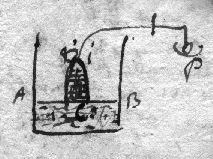
\includegraphics[width=0.90\textwidth]{images/LH035,14,02_122v_Ausschnitt.pdf}\\
\\
\noindent\centering\hspace*{-18mm}[\textit{Fig. 23}]
\end{minipage}
\hspace*{-2mm}
\begin{minipage}[t]{0.61\textwidth}
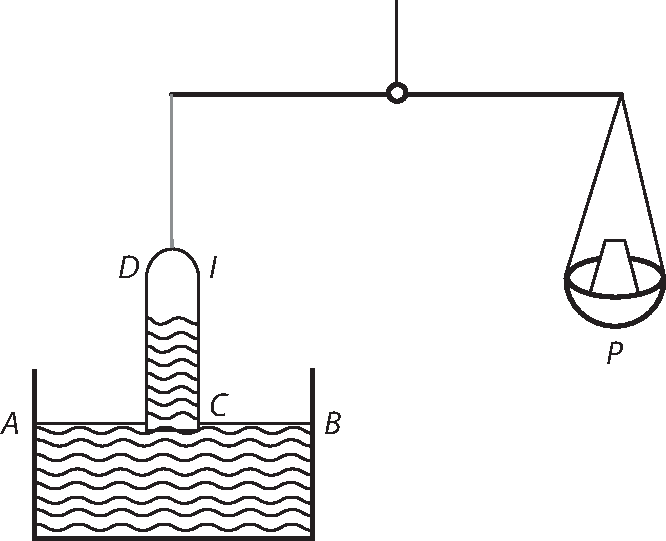
\includegraphics[width=0.90\textwidth]{images/LH035,14,02_122v-d1.pdf}\\
\\
\noindent\centering\hspace*{-2mm}[\textit{Fig. 24, erg. Hrsg. nach Wallis}]
\vspace{1em}
\end{minipage}
\edtext{}{\lemma{\hspace*{1,8mm}[\textit{Fig. 24}]}\killnumber\Cfootnote{\hspace{-1mm}Leibniz' Abzeichnung [\textit{Fig. 23}] nach Vorlage verbessert. Vgl. \cite{00301}a.a.O., Fig. 319 (\cite{01008}\textit{WO} I, S. 1040).}}%
\pend
\vspace*{1em}% PR: Rein provisorisch !!!!
\pstart
Cap. XIV. \setline{1}de Hydrostaticis\protect\index{Sachverzeichnis}{hydrostatica}.
Ubi et de Hydrargyro\protect\index{Sachverzeichnis}{hydrargyrum} suspenso.\\
\hspace*{7,5mm}\edtext{\textit{Si intelligatur tubi\protect\index{Sachverzeichnis}{tubum}
fundus $\displaystyle D.$ fili\protect\index{Sachverzeichnis}{filum} ope
de libra\protect\index{Sachverzeichnis}{libra} pendere}
posito \textit{ex adverso} pondere\protect\index{Sachverzeichnis}{pondus} $\displaystyle P.$
\textit{quo hoc tubo gravato aequiponderet;
requiritur ut aequet pondere tum tubi pondus,
% [...]
tum tantum hydrargyri\protect\index{Sachverzeichnis}{hydrargirum}
quantum aequet cylindrum $\displaystyle CI.$}}{%
\lemma{\textit{Si intelligatur} [...] \textit{cylindrum $\displaystyle CI$}}%
\Cfootnote{\cite{00301}a.a.O., cap. 14, prop. 10, S. 722 (\cite{01008}\textit{WO} I, S. 1040). Zitat mit Auslassungen.\hspace{-4mm}}}
%
\pend
%\newpage% PR: Rein provisorisch !!!!
\vspace*{1em}% PR: Rein provisorisch !!!!
\count\Afootins=1200
\count\Bfootins=1200
\count\Cfootins=1200
%%%%%%%%%%%%%%%%%%%%
%\vspace*{1.5em}% PR: Rein provisorisch !!!!
%\newpage% PR: Rein provisorisch !!!!
\pstart
Ad prop. XI. schol.
\edtext{\textit{Jam ante sex annos tubum 4 pedes longum cum semisse
implendum curavi Hydrargyro ab intermisto aere\protect\index{Sachverzeichnis}{aer} diligenter purgato
(non summa tamen diligentia,}%
[\textit{)}]\edtext{}{\lemma{\textit{)}}\Bfootnote{\textit{erg. Hrsg. nach Vorlage}}}
\textit{eumque sic impletum inverti obturato primum diligenter orificio,
nec prius recluso, quam}
[\textit{infra}]\edtext{}{\lemma{intra}\Bfootnote{\textit{L ändert Hrsg. nach Vorlage}}}
\textit{superficiem Hydrargyri in subjecto vase\protect\index{Sachverzeichnis}{vas} contenti demergeretur,
deinde facta subtus} effluendi \textit{potestate effluxit
Hydrargyri\protect\index{Sachverzeichnis}{hydrargyrum} tubo\protect\index{Sachverzeichnis}{tubum} contenti pars magna
cum impetu\protect\index{Sachverzeichnis}{impetus} notabili,
factisque ob impetum illum vibrationibus\protect\index{Sachverzeichnis}{vibratio} aliquot,
subsistebat tandem ad altitudinem Unciarum\protect\index{Sachverzeichnis}{uncia Anglicana}
pedis Anglicani,\protect\index{Sachverzeichnis}{pes Anglicanus} (plus minus) 29.
Tubumque cum subjecto vase,\protect\index{Sachverzeichnis}{vas} cujus fundo nitebatur apertum tubi orificium,
sed ita ut exeundi et intrandi a vase\protect\index{Sachverzeichnis}{vas} in tubum
Hydrargyro\protect\index{Sachverzeichnis}{hydrargyrum}}
\textit{via non intercluderetur,
in pegma quoddam prius ad id paratum intuli
atque in hunc diem in eo statu conservo.}
% S. 727f. / 1043
At \textit{a Calendis Januariis anni exeuntis 1664 ineuntis 1665,}
cum domi sum, Ephemeridem\protect\index{Sachverzeichnis}{ephemeris} instituo.
Observo autem semper esse supra uncias
[viginti]\edtext{}{\lemma{viginti}\Bfootnote{\textit{erg. Hrsg. nach Vorlage}}}
octo pedis Anglicani,\protect\index{Sachverzeichnis}{pes Anglicanus}
semper infra uncias\protect\index{Sachverzeichnis}{uncia Anglicana} 30,
\textit{semel autem iterumque tantillo super 30}
\edtext{\textit{ascenderat,} et}{%
\lemma{\textit{ascenderat,}}\Bfootnote{%
\textit{(1)}\ \textit{}sed
\textit{(2)}\ \textit{}et
\textit{L}}}
% S. 728 / 1043f.
semel iterumque tantillo
[subsiderat infra 28.]\edtext{}{\lemma{subsiderat infra 28.}\Bfootnote{\textit{erg. Hrsg. nach Vorlage}}}
Altitudinem in Tubo\protect\index{Sachverzeichnis}{tubum Boylii} Boylii,\protect\index{Namensregister}{\textso{Boyle} (Boylius, Boyl), Robert 1627-1691}
tum Oxonii\protect\index{Ortsregister}{Oxford} ageret[,] aliquando deprehendi mea majorem,
\textit{quasi octava parte unius unciae si} bene \textit{memini,
sive quod} Mercurius\protect\index{Sachverzeichnis}{Mercurius} ejus levior,
sive quod alter altero aliquanto depuratior.
\textit{A Scriptoribus Gallis assignari} solent \textit{unciae 27 pedis Parisini.}
% S. 728 / 1044
Sed pes Parisinus\protect\index{Sachverzeichnis}{pes Parisinus} superat Anglicanum\protect\index{Sachverzeichnis}{pes Anglicanus} $\displaystyle\frac{4}{5}$\textsuperscript{tis} unciae nostrae (pedis Anglicani,)
\textit{adeoque unciae Parisinae\protect\index{Sachverzeichnis}{uncia Parisina} 
27 respondent nostris\protect\index{Sachverzeichnis}{uncia Anglicana} 29 quam proxime.}
\protect\rule[-4mm]{0mm}{10mm}$\displaystyle \frac{12}{12\frac{4}{5}} \sqcap \frac{60}{64} \sqcap \frac{27}{28\frac{4}{5}}.$}{%
\lemma{\textit{Jam} [...] $\displaystyle \sqcap \frac{27}{28\frac{4}{5}}$}%
\Cfootnote{\cite{00301}a.a.O., S. 727f. (\cite{01008}\textit{WO} I, S. 1043f.). Zitat mit Auslassungen.}}
%
\pend
\vspace*{1mm}
\pstart
\edtext{\textit{Vis aeris\protect\index{Sachverzeichnis}{aer} Elastica\protect\index{Sachverzeichnis}{vis elastica} vase inclusi,
tantundem praestat}, quantum pondus aperti.}{%
\lemma{\textit{Vis} [...] aperti}%
\Cfootnote{\hspace{-0.7mm}\cite{00301}a.a.O., S. 730 (\cite{01008}\textit{WO} I, S. 1045). Zitat m. Auslassungen.\hspace{-4mm}}}
\edtext{}{\lemma{}\Afootnote{\textit{Am Rand:}
% 550,000 ad 1.
Summa\textsuperscript{[a]} dilatatio aeris nota ad summam compressionem\textsuperscript{[b]} ut 550,000 ad 1.\textsuperscript{[c]}
\vspace{2mm}\\
\footnotesize
\textsuperscript{[a]}
summa
\textit{(1)}\ expansio
\textit{(2)}\ dilatatio
\textit{L}
\quad \quad
\textsuperscript{[b]}
compressionem
\textit{(1)}\ ut 500,000 ad 1
\textit{(2)}\ 550,000 ad 1
\textit{L}
\quad
\textsuperscript{[c]}
ut 550,000 ad 1:
\cite{00301}J. \textsc{Wallis}, \textit{Mechanica}, pars III, cap.14 , London 1670-1671, S. 738 (\cite{01008}\textit{WO} I, S. 1050.).
\vspace{-8mm}% PR: Rein provisorisch.
}}
\pend
\count\Afootins=1200
\count\Bfootins=1200
\count\Cfootins=1200
\pstart
\edtext{\textit{Observavit Boylius\protect\index{Namensregister}{\textso{Boyle} (Boylius, Boyl), Robert 1627-1691}
paradoxis Hydrostaticis in fine
in Gyrinis,\protect\index{Sachverzeichnis}{gyrinus} nostrates, alibi Tad-poles appellant, alibi Hob-nails}[,]
\textit{aqua\protect\index{Sachverzeichnis}{aqua} inclusis valide}
\edtext{compressis,}{%
\lemma{compressis}%
\Cfootnote{In der Vorlage \textit{compressa}.}}
\textit{ubi se satis vivide movebant, sed magnitudine minuta.}}{%
\lemma{\textit{Observavit} [...] \textit{minuta}}%
\Cfootnote{\cite{00301}a.a.O., S. 734 (\cite{01008}\textit{WO} I, S. 1047).
Siehe R.\cite{00239} \textsc{Boyle}, \textit{Hydrostatical Paradoxes}, Oxford 1666, S. 244-247.}}
%
\edtext{Sanguis\protect\index{Sachverzeichnis}{sanguis}
in antlia\protect\index{Sachverzeichnis}{antlia Boyliana} Boyliana\protect\index{Namensregister}{\textso{Boyle} (Boylius, Boyl), Robert 1627-1691}
\edtext{mire spumescit,}{%
\lemma{mire}\Bfootnote{%
\textit{(1)}\ bullescit
\textit{(2)}\ spumescit
\textit{L}}}
imo \textit{in amplissimas bullas\protect\index{Sachverzeichnis}{bulla} se expandit
% [...]
ita ut saponis\protect\index{Sachverzeichnis}{sapo} inter lavandum expansio in bullas huic}
\edtext{[\textit{aeris in sanguine expansioni}]}{\lemma{\textit{aeris} [...] \textit{expansioni}}\Bfootnote{\textit{erg. Hrsg. nach Vorlage}}}
\textit{cedat.
Quodque inde rumpantur fibrae},\protect\index{Sachverzeichnis}{fibra}
vel hinc aestimes,
quod sanguis\protect\index{Sachverzeichnis}{sanguis} qui in grumosam massam coaluisset alioqui,
postea in aere libero liquidus permanet.}{%
\lemma{Sanguis [...] permanet}%
\Cfootnote{J.\cite{00301} \textsc{Wallis}, \textit{Mechanica}, pars III, cap. 14, London 1670-1671, S. 734 (\cite{01008}\textit{WO} I, S. 1047). Zitat mit Auslassungen.}}
%
\edtext{Aer\protect\index{Sachverzeichnis}{aer} in experimentis Florentinis
\textit{absque caloris\protect\index{Sachverzeichnis}{calor} ope}[,]
\textit{solius experimenti\protect\index{Sachverzeichnis}{experimentum Torricellianum}
Torricelliani\protect\index{Namensregister}{\textso{Torricelli}, Evangelista 1608-1647} auxilio expansus,
in molem 173 vicibus pristina majorem.}}{%
\lemma{Aer [...] \textit{majorem}}%
\Cfootnote{\cite{00301}a.a.O., S. 737 (\cite{01008}\textit{WO} I, S. 1049).
Siehe L.\cite{00143} \textsc{Magalotti}, \textit{Saggi di naturali esperien\-ze}, Florenz 1667, S. 40-46.}}
%
\edtext{In machina compressiva\protect\index{Sachverzeichnis}{machina compressiva} societatis regiae,\protect\index{Sachverzeichnis}{Royal Society}
\textit{aer in spatii soliti partem 10 vel 12 etiam} compressus.}{%
\lemma{In machina [...] compressus}%
\Cfootnote{J.\cite{00301} \textsc{Wallis}, \textit{Mechanica}, pars III, cap. 14, London 1670-1671, S. 737 (\cite{01008}\textit{WO} I, S. 1049).}}
%
\edtext{At Boylius\protect\index{Namensregister}{\textso{Boyle} (Boylius, Boyl), Robert 1627-1691} frigore
(circumponendo vasi\protect\index{Sachverzeichnis}{vas}
\edtext{vitreo}{\lemma{vitreo}\Bfootnote{\textit{erg. L}}}
glaciem\protect\index{Sachverzeichnis}{glacies} sale\protect\index{Sachverzeichnis}{sal} mixtam
\textit{eo modo qui in}
\edtext{congelata}{\lemma{congelata}\Cfootnote{In der Vorlage \textit{congelanda}.}}
\textit{aqua adhiberi solet})
% 737 / 1049
contractum aerem\protect\index{Sachverzeichnis}{aer} reperit
\textit{in spatium quod erat ad pristinum ut}
11 \textit{ad 158 plus}
[\textit{minus},]\edtext{}{\lemma{\textit{minus},}\Bfootnote{\textit{erg. Hrsg. nach Vorlage}}}
aqua\protect\index{Sachverzeichnis}{aqua} immissa
quae frigore\protect\index{Sachverzeichnis}{frigor} expandebatur,
circummissa glacie vel nive\protect\index{Sachverzeichnis}{nivis} sale
\edtext{mixta contractus}{%
\lemma{mixta}\Bfootnote{%
\textit{(1)}\ expansus est
\textit{(2)}\ contractus
\textit{L}}}
\protect\rule[-4mm]{0mm}{10mm}aer\protect\index{Sachverzeichnis}{aer} in partem $\displaystyle\frac{1}{40}.$}{%
\lemma{At Boylius [...] $\displaystyle\frac{1}{40}$}%
\Cfootnote{\cite{00301}a.a.O., S. 737f. (\cite{01008}\textit{WO} I, S. 1049).}}
%
[123~r\textsuperscript{o}] %%%%%%%%%%  HIER BEGINNT BLATT 123r. 
%
\pend
\pstart
Prop. XIII de Hydrostaticis,\protect\index{Sachverzeichnis}{hydrostatica} Scholio prop.
[XIII]\edtext{}{\lemma{XII}\Bfootnote{\textit{L ändert Hrsg.}}}
refert \edtext{experimentum illud notabile publicatum ab Hugenio.\protect\index{Namensregister}{\textso{Huygens} (Hugenius, Ugenius, Hugens, Huguens), Christiaan 1629-1695}}{%
\lemma{experimentum [...] Hugenio}%
\Cfootnote{C.\cite{00062} \textsc{Huygens}, \textit{Extrait d'une lettre}, \textit{JS} (1672), S. 134f. (\cite{00113}\textit{HO} VII, S. 202f.).
Siehe hierzu \textit{LSB} VIII, 1 N. 39.\cite{01069}}}
%
\edtext{%
\textit{Observaverat Boylius}\protect\index{Namensregister}{\textso{Boyle} (Boylius, Boyl), Robert 1627-1691}
ut \textit{ex Experimentis ejus Physico-Mechanicis anno 60 editis, Experimento 17. ante monuimus;
Hydrargyrum}\protect\index{Sachverzeichnis}{hydrargyrum}
\edtext{in}{\lemma{in}\Cfootnote{In der Vorlage \textit{intra}.}}
\textit{antliam\protect\index{Sachverzeichnis}{antlia} suam
Tubo\protect\index{Sachverzeichnis}{tubum} suspensum,
subducto aere\protect\index{Sachverzeichnis}{aer} gradatim descendere,
% [...]
non ita tamen quin} quacunque adhibita diligentia
\textit{supra stagnantis inferius} Mercurii\protect\index{Sachverzeichnis}{mercurius}
\textit{superficiem contra quam speraverat
extaret adhuc ad altitudinem unciae\textso{ vel saltem semiunciae }%
(praesertim si ab aere prius depuratum fuerat)
cui in aqua\protect\index{Sachverzeichnis}{aqua} respondent 
pedis\protect\index{Sachverzeichnis}{pes} unciae\protect\index{Sachverzeichnis}{uncia} minimum 7 aut 8.
Idemque in aqua expertus immissis in antliam tubis brevibus,
puta, 5 aut 6 unciarum pedis, ea repletis,
aquam reperit, saltem si ab aere prius depurgata fuerat,
non \edlabel{035,14,02_123r_z1}%
\edtext{}{{\xxref{035,14,02_123r_z1}{035,14,02_123r_z2}}%
\lemma{\textit{descendere.}}\Bfootnote{%
\textit{(1)}\ \textit{Idem in aqua expertus immissis in antliam tubis brevibus puta 5 aut 6 unciarum}
\textit{(2)}\ Cumque Hugenius
\textit{(a)}\ viso libro ann
\textit{(b)}\ visa Machina Boyliana
\textit{L}}}%
descendere.}}{%
\lemma{\textit{Observaverat} [...] \textit{descendere}}%
\Cfootnote{J.\cite{00301} \textsc{Wallis}, \textit{Mechanica}, pars III, cap. 14, London 1670-1671, S. 739 (\cite{01008}\textit{WO} I, S. 1050). Zitat mit Auslassungen.
Siehe R.\cite{00015} \textsc{Boyle}, \textit{New experiments physico-mechanicall}, Oxford 1660, S. 106-129% (\cite{00017}\textit{BW} I, S. ????)
.}}\edtext{
% 1670-1671, S. 739 (WO I, S. 1050)
%
Cumque Hugenius\protect\index{Namensregister}{\textso{Huygens} (Hugenius, Ugenius, Hugens, Huguens), Christiaan 1629-1695}
visa \protect\index{Sachverzeichnis}{machina Boyliana}Machina Boyliana\edlabel{035,14,02_123r_z2}
similem domi elaborare curasset,
idem \textit{immisso in antliam tubo breviusculo} deprehendit idque
\textit{\edtext{suis literis}{\lemma{suis literis}\Cfootnote{Insbesondere Huygens Briefe an R. Moray Nr. 963 (3. Februar 1662)\cite{01074} und Nr. 1032 (14. Juli 1662)\cite{01075} mit der Beilage Nr. 1033\cite{01076} in \textit{HO} IV, S. 23-25 und 171-175.\cite{00113}}}
ut notabilem in doctrina Boyliana
% [...]
difficultatem objecit.
Cui \edtext{respondit Boylius\protect\index{Namensregister}{\textso{Boyle} (Boylius, Boyl), Robert 1627-1691}}{\lemma{respondit Boylius}\Cfootnote{Siehe den Brief Nr. 1056 (R. Boyle an R. Moray, Juli 1662)\cite{01077} in \textit{HO} IV, S. 217-220.\cite{00113}}}
rem plane ita esse,}
videri autem oriri ex eo quod antlia\protect\index{Sachverzeichnis}{antlia}
non penitus aere\protect\index{Sachverzeichnis}{aer} exhausta.}{%
\lemma{Cumque [...] exhausta}%
\Cfootnote{J.\cite{00301} \textsc{Wallis}, \textit{Mechanica}, pars III, cap. 14, London 1670-1671, S. 739f. (\cite{01008}\textit{WO} I, S. 1050f.). Zitat mit Auslassungen.}}
%
%\edtext{%
%\textit{Observaverat Boylius}\protect\index{Namensregister}{\textso{Boyle} (Boylius, Boyl), Robert 1627-1691}
%ut \textit{ex Experimentis ejus Physico-Mechanicis anno 60 editis, Experimento 17. ante monuimus;
%Hydrargyrum}\protect\index{Sachverzeichnis}{hydrargyrum}
%\edtext{in}{\lemma{in}\Cfootnote{In der Vorlage \textit{intra}.}}
%\textit{antliam\protect\index{Sachverzeichnis}{antlia} suam
%Tubo\protect\index{Sachverzeichnis}{tubum} suspensum,
%subducto aere\protect\index{Sachverzeichnis}{aer} gradatim descendere,
%% [...]
%non ita tamen quin} quacunque adhibita diligentia
%\textit{supra stagnantis inferius} Mercurii\protect\index{Sachverzeichnis}{mercurius}
%\textit{superficiem contra quam speraverat
%extaret adhuc ad altitudinem unciae\textso{ vel saltem semiunciae }%
%(praesertim si ab aere prius depuratum fuerat)
%cui in aqua\protect\index{Sachverzeichnis}{aqua} respondent 
%pedis\protect\index{Sachverzeichnis}{pes} unciae\protect\index{Sachverzeichnis}{uncia} minimum 7 aut 8.
%Idemque in aqua expertus immissis in antliam tubis brevibus,
%puta, 5 aut 6 unciarum pedis, ea repletis,
%aquam reperit, saltem si ab aere prius depurgata fuerat,
%non descendere.}}{%
%\lemma{\textit{Observaverat} [...] \textit{descendere}}%
%\Cfootnote{J.\cite{00301} \textsc{Wallis}, \textit{Mechanica}, pars III, cap. 14, London 1670-1671, S. 739 (\cite{01008}\textit{WO} I, S. 1050). Zitat mit Auslassungen.
%Siehe R.\cite{00015} \textsc{Boyle}, \textit{New experiments physico-mechanicall}, Oxford 1660, S. 106-129% (\cite{00017}\textit{BW} I, S. ????)
%.}}\edtext{
%% 1670-1671, S. 739 (WO I, S. 1050)
%\edtext{%
%Cumque Hugenius\protect\index{Namensregister}{\textso{Huygens} (Hugenius, Ugenius, Hugens, Huguens), Christiaan 1629-1695}
%visa Machina Boyliana\protect\index{Sachverzeichnis}{machina Boyliana}}{%
%\lemma{\textit{descendere.}}\Bfootnote{%
%\textit{(1)}\ \textit{Idem in aqua expertus immissis in antliam tubis brevibus puta 5 aut 6 unciarum}
%\textit{(2)}\ Cumque Hugenius
%\textit{(a)}\ viso libro ann
%\textit{(b)}\ visa Machina Boyliana
%\textit{L}}}
%similem domi elaborare curasset,
%idem \textit{immisso in antliam tubo breviusculo} deprehendit idque
%\textit{\edtext{suis literis}{\lemma{suis literis}\Cfootnote{Insbesondere Huygens Briefe an R. Moray Nr. 963 (3. Februar 1662)\cite{01074} und Nr. 1032 (14. Juli 1662)\cite{01075} mit der Beilage Nr. 1033\cite{01076} in \textit{HO} IV, S. 23-25 und 171-175.\cite{00113}}}
%ut notabilem in doctrina Boyliana
%% [...]
%difficultatem objecit.
%Cui \edtext{respondit Boylius\protect\index{Namensregister}{\textso{Boyle} (Boylius, Boyl), Robert 1627-1691}}{\lemma{respondit Boylius}\Cfootnote{Siehe den Brief Nr. 1056 (R. Boyle an R. Moray, Juli 1662)\cite{01077} in \textit{HO} IV, S. 217-220.\cite{00113}}}
%rem plane ita esse,}
%videri autem oriri ex eo quod antlia\protect\index{Sachverzeichnis}{antlia}
%non penitus aere\protect\index{Sachverzeichnis}{aer} exhausta.}{%
%\lemma{Cumque [...] exhausta}%
%\Cfootnote{J.\cite{00301} \textsc{Wallis}, \textit{Mechanica}, pars III, cap. 14, London 1670-1671, S. 739f. (\cite{01008}\textit{WO} I, S. 1050f.). Zitat mit Auslassungen.}}
%
\edtext{%
Sed re postea amplius discussa
reperit Brounckerus\protect\index{Namensregister}{\textso{Brouncker} (Brunckerus), William Viscount 1620-1684}
\textit{se Hydrargyrum\protect\index{Sachverzeichnis}{hydrargyrum} sic suspensum tenuisse
ultra solitam altitudinem ad aequipondium necessariam, 29} vel \textit{30.
% 1670-1671, S. 740 (WO I, S. 1051)
Nempe ad uncias\protect\index{Sachverzeichnis}{uncia} usque 34.}
Boylius\protect\index{Namensregister}{\textso{Boyle} (Boylius, Boyl), Robert 1627-1691}
idem in altitudine unciarum 52.
Tandem \edtext{Praeses\protect\index{Namensregister}{\textso{Brouncker} (Brunckerus), William Viscount 1620-1684}}{%
\lemma{Praeses}\Cfootnote{William Brouncker, 1662 bis 1677 Vorsitzender der Royal Society.}}
in altitudine 55.
pollicitus se rem porro tentaturum.
\textit{Quae} \edtext{\textit{ex regestis Societatis\protect\index{Sachverzeichnis}{Royal Society} anno 1662. 1663 liquent.}}{\lemma{\textit{ex} [...] \textit{liquent}}\Cfootnote{Keine spezifischen Berichte über diese Messungen lassen sich in den ersten Heften der \textit{PT} (1665-1670) ermitteln. Siehe aber den Brief Nr. 1171 (R. Boyle an H. Oldenburg, 8. Novemeber 1663)\cite{01078} in \textit{HO} IV, S. 437-440.\cite{00113}}}
% 1670-1671, S. 740 (WO I, S. 1051)
Inde frequenti experientia deprehensum ad 60 usque et plures uncias suspendi,
\textit{atque ita suspensum}
[\textit{per}]\edtext{}{\lemma{ad}\Bfootnote{\textit{L ändert Hrsg. nach Vorlage.}}}
\textit{dies aliquot consistere,
sed concussione facta,
vel tantillo aere admisso,
statim praecipitari ad}
\edtext{fundum.}{\lemma{fundum}\Cfootnote{In der Vorlage \textit{Aequilibrium}.}}}{%
\lemma{Sed re [...] fundum}%
\Cfootnote{J.\cite{00301} \textsc{Wallis}, \textit{Mechanica}, pars III, cap. 14, London 1670-1671, S. 740 (\cite{01008}\textit{WO} I, S. 1051).}}
%
\edtext{%
\textit{Suspicatur Brounckerus\protect\index{Namensregister}{\textso{Brouncker} (Brunckerus), William Viscount 1620-1684}
aeris\protect\index{Sachverzeichnis}{aer} pondus\protect\index{Sachverzeichnis}{pondus} multo majus esse,
quam ut altitudini Hydrargyri unciarum\protect\index{Sachverzeichnis}{uncia} plus minus 29 respondeat,
sed ab aere intus latente, nisi expurgetur,
ad eam usque altitudinem}
\edtext{depressum}{\lemma{depressum}\Cfootnote{In der Vorlage (irrtümlich) \textit{depressam}.}}
\textit{esse hydrargyrum.\protect\index{Sachverzeichnis}{hydrargirium}
At ubi expurgatur aer nihilque tum supersit quod externi aeris ponderi se opponat,
praeter nudum hydrargyri pondus, rem secus deprehendi};
et \textit{hydrargyrum ab aeris aequipondio altius sustineri.}}{%
\lemma{\textit{Suspicatur} [...] \textit{sustineri}}%
\Cfootnote{\cite{00301}J.\cite{00301} \textsc{Wallis}, \textit{Mechanica}, pars III, cap. 14, London 1670-1671, S. 741f. (\cite{01008}\textit{WO} I, S. 1052).}}
% 
(+~Hoc obscure.~+)
\pend
\count\Afootins=1100
\count\Bfootins=1100
\count\Cfootins=1100
\pstart
\edtext{%
Pondus [aquae]\edtext{}{\lemma{Hydrargyri}\Bfootnote{\textit{L ändert Hrsg. nach Vorlage}}}
est ad pondus [Hydrargyri]\edtext{}{\lemma{aquae}\Bfootnote{\textit{L ändert Hrsg. nach Vorlage}}}
ut 1 ad 14 seu potius
ut Boylius\protect\index{Namensregister}{\textso{Boyle} (Boylius, Boyl), Robert 1627-1691}
ex suis \edtext{experimentis, ad \protect\rule[-4mm]{0mm}{10mm}$\displaystyle 13 \frac{3}{4}.$}{%
\lemma{experimentis,}\Bfootnote{%
\textit{(1)}\ ut $\displaystyle 13 \frac{3}{4}$ ad
\textit{(2)}\ ad $\displaystyle 13 \frac{3}{4}$
\textit{L}}}
Marinus Getaldus\protect\index{Namensregister}{\textso{Ghetaldi} (Getaldus), Marino 1566-1626} in \textit{Archimede promoto}
%
$\displaystyle 13 \frac{4}{7}.$
Boylius\protect\index{Namensregister}{\textso{Boyle} (Boylius, Boyl), Robert 1627-1691}
in \textit{Conti\-nuatione Experimentorum Physico-Mechanicorum} Experim. 15.
%
\textit{quo tempore altitudo \mercury\textsuperscript{ii}\protect\index{Sachverzeichnis}{Mercurius}
propter athmosphaerae aequipondium suspensi
\edtext{fuit unciarum pedis\protect\index{Sachverzeichnis}{pedes} \protect\rule[-4mm]{0mm}{10mm}$\displaystyle 29 \frac{1}{4}$ proxime,}{%
\lemma{fuit}\Bfootnote{%
\textit{(1)}\ \textit{}pedum 33 unciarum  6. hoc est pedum $\displaystyle 33 \frac{1}{2}$
\textit{(2)}\ \textit{unciarum} [...] \textit{proxime,}
\textit{L}}}}
% 1670-1671, 742 / WO I, 1052
aqua\protect\index{Sachverzeichnis}{aqua} suctione elevari potuit ad pedes 33 uncias 6.
Nam si multiplices uncias \protect\rule[-4mm]{0mm}{10mm}$\displaystyle 29\frac{1}{4}$ per $\displaystyle 13\frac{3}{4}$
habebis uncias 402 proxime, seu 33 cum 6 unciis.}{%
\lemma{Pondus [...] unciis}%
\Cfootnote{\cite{00301}a.a.O., S. 742 (\cite{01008}\textit{WO} I, S. 1052). Siehe R.\cite{01062} \textsc{Boyle}, \textit{A Continuation of New Experiments Physico-Mechanical}, Oxford 1669, S. 45.  M.\cite{00312} \textsc{Ghetaldi}, \textit{Promotus Archimedis, seu De variis corporum generibus gravitate et magnitudine comparatis}, Rom 1603, S. 32.}}
%
\pend
%\vspace*{0.5em}
\newpage% PR: Rein provisorisch !!!
\count\Afootins=1200
\count\Bfootins=1500
\count\Cfootins=1500
\pstart
\begin{wrapfigure}[22]{l}{0.28\textwidth}
\vspace{-5mm}
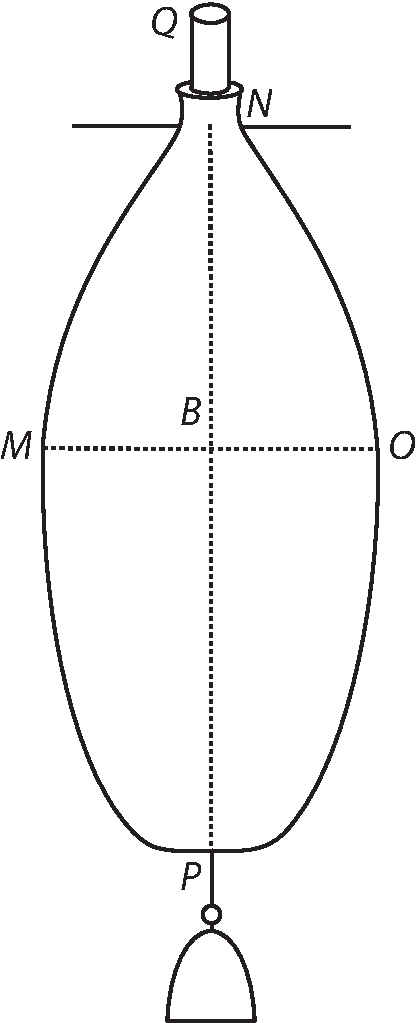
\includegraphics[trim = 0mm -2mm -5mm 0mm, clip, width=0.28\textwidth]{images/LH035,14,02_123r-d1.pdf}\\
\noindent \centering [\textit{Fig. 25, erg. Hrsg. nach Wallis}]\edtext{}{\lemma{\hspace*{1,8mm}[\textit{Fig. 25}]}\killnumber\Cfootnote{Vgl. \cite{00301}a.a.O., Fig. 333 (\cite{01008}\textit{WO} I, S. 1056).}}
\end{wrapfigure}
In Epilogo ex Miscellaneis prop. 3. habet%
\edtext{}{\lemma{}\Afootnote{\textit{Am Rand:} Vis\protect\index{Sachverzeichnis}{vis} flatus\protect\index{Sachverzeichnis}{flatus}
aequalis vi musculorum\protect\index{Sachverzeichnis}{musculus} pectus\protect\index{Sachverzeichnis}{pectus} comprimentium.}}
Wallisius\protect\index{Namensregister}{\textso{Wallis} (Wallisius), John 1616-1703}
\edtext{%
se vidisse Oxoniae\protect\index{Ortsregister}{Oxford} 1651 in conventu studiosorum institutum
\edtext{experimentum,\protect\index{Sachverzeichnis}{experimentum} (non ut novum, sed ut vetus[,] ut repetendum).}{%
\lemma{experimentum,}\Bfootnote{%
\textit{(1)}\ ut saepius repetiturum
\textit{(2)}\ (non [...] repetendum)
\textit{L}}}
Nempe si vesicae\protect\index{Sachverzeichnis}{vesica}
\textit{cervix pegmati\protect\index{Sachverzeichnis}{pegma} seu}
\edtext{\textit{fulcro\protect\index{Sachverzeichnis}{fulcrum}} alicubi}{%
\lemma{\textit{fulcro}}\Bfootnote{%
\textit{(1)}\ aliquo
\textit{(2)}\ alicubi
\textit{L}}}
\textit{firmo figatur,
ita tamen ut per calamum seu fistulam $\displaystyle Q$ inflari possit
fundoque affigatur pondus $\displaystyle P,$
experimento\protect\index{Sachverzeichnis}{experimentum} compertum est
flatu spiritus humani\protect\index{Sachverzeichnis}{flatus}
inflata vesica\protect\index{Sachverzeichnis}{vesica} adeoque lateribus distentis et longitudine contracta
pondus\protect\index{Sachverzeichnis}{pondus} librarum\protect\index{Sachverzeichnis}{libra} 50. 60. 70. aut etiam plurium
% [...]
notabiliter} (+~explicanda erat quantitas,
circiter~+) \textit{elevari posse.}
% 1670-1671, 759.
Considerandum \textit{ad quantam distantiam et quam celeri fortique motu,
globus argillaceus\protect\index{Sachverzeichnis}{globus argillaceus} flando expelli soleat
ex tubo oblongo\protect\index{Sachverzeichnis}{tubum}
quali in occidendis avibus\protect\index{Sachverzeichnis}{avis} utuntur.}
% 1670-1671, 759.
Praesertim cum hic magna spiritus copia parum attollatur pondus\protect\index{Sachverzeichnis}{pondus}}{%
\lemma{se vidisse [...] pondus}%
\Cfootnote{J.\cite{00301} \textsc{Wallis}, \textit{Mechanica}, pars III, cap. 15, London 1670-1671, S. 759 (\cite{01008}\textit{WO} I, S. 1056). Zitat mit Auslassungen.}}
%
(+~potuisset vesica immergi Hydrargyro, et inde inflari~+).\\
%\newpage% PR: Rein provisorisch !!!
%\vspace*{1.0em}% PR: Rein provisorisch !!!!
%%%%%%%%%%%%%%%%%%%% PR: Bitte, Abbildungen korrekt setzen. Danke.
%\pstart
% \vspace*{2em}
%\noindent\centering
%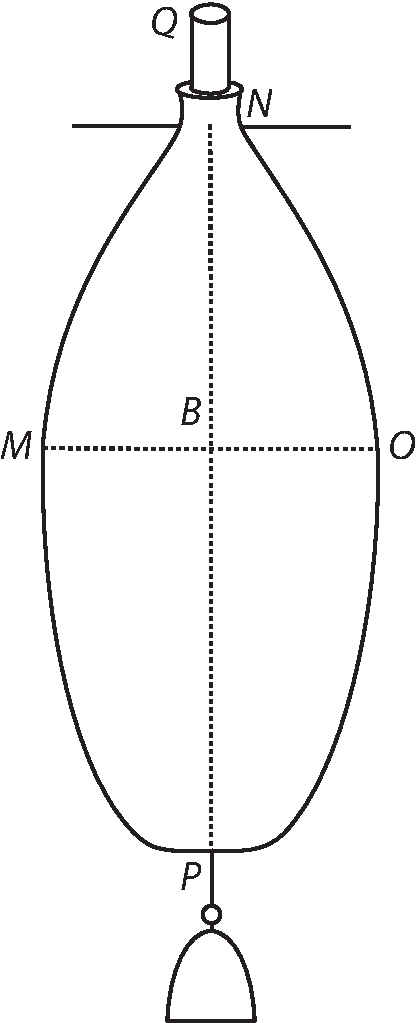
\includegraphics[width=0.3\textwidth]{images/LH035,14,02_123r-d1.pdf}\\%
%\vspace*{1.0em}%
%[\textit{Fig. 25, erg. Hrsg. nach Wallis}]\edtext{}{\lemma{\hspace*{1,8mm}[\textit{Fig. 25}]}\killnumber\Cfootnote{Vgl. \cite{00301}a.a.O., Fig. 333 (\cite{01008}\textit{WO} I, S. 1056).}}
%\newpage
%\vspace*{2.0em}%
\hspace*{7.0mm}
Subjiciuntur\textso{ quaestiones aliquot  Mechanicae.}\\
\hspace*{7.0mm}
\edtext{%
\textit{Cur qui ad erectum murum\protect\index{Sachverzeichnis}{murus} stat erectus,
dorso et utrisque calcibus murum attingens,
non potest nisi promoto pedum\protect\index{Sachverzeichnis}{pes} altero
nummum\protect\index{Sachverzeichnis}{nummus} humi jacentem prorsum incurvatus tollere
quin} praecipitetur[?]
\textit{Ratio petenda a situ centri gravitatis\protect\index{Sachverzeichnis}{centrum gravitatis}:
quippe cum fulcrum\protect\index{Sachverzeichnis}{fulcrum} corporis sit in pedibus,
qui cadere non volet hoc curare debet,
ut totius corporis centrum gravitatis pedibus emineat,
saltem non extra eorum extrema hac vel illac ulterius deflectat,
quam ut musculorum\protect\index{Sachverzeichnis}{musculus}
ac tendinum\protect\index{Sachverzeichnis}{tendo} vires\protect\index{Sachverzeichnis}{vis}
sic positum sustinere valeant et revocare.}
% 1670-1671, 767 / WO I, 1061
(+~Hinc vis illa musculorum et tendinum mensurari poterit,
\edtext{ex quanta scilicet altitudine}{%
\lemma{ex}\Bfootnote{%
\textit{(1)}\ eo
\textit{(2)}\ quanta scilicet altitudine
\textit{L}}}
possit elevare nummum, ita ut non cadat.~+)
\textit{Hinc qui erectus stat, stat firmus,
utpote qui totam corporis molem\protect\index{Sachverzeichnis}{molis} habet pedibus supereminentem.
Qui vero quid humi tollere vult dum demissum caput protendit antrorsum,
nates retrorsum tendit, quo fiat aequilibrium,
centrumque totius pedibus seu fulcro superemineat,}
aut \textit{extra pedum\protect\index{Sachverzeichnis}{pes} ambitum}
parum \textit{deflectat.}
% 1670-1671, 767 / WO I, 1061
Sed quia in nostro casu propter murum\protect\index{Sachverzeichnis}{murus} hoc non potest,
\textit{praecipitatur} si \textit{totius centrum positum
extra fulcrum seu fulcrorum\protect\index{Sachverzeichnis}{fulcrum}
\edtext{extremum ambitum,}{%
\lemma{extremum}\Bfootnote{%
\textit{(1)}\ ambigum
\textit{(2)}\ \textit{ambitum}
\textit{L}}}
magis quam ut valeant tendines id oneris\protect\index{Sachverzeichnis}{onus} ferre
iterumque sublevare.
Saltem nisi vertebrarum\protect\index{Sachverzeichnis}{vertebra} tendines\protect\index{Sachverzeichnis}{tendo}
musculique\protect\index{Sachverzeichnis}{musculus} eo spectantes admodum robusti fuerint.
Hinc est etiam, quod alii fortius alii mollius terram\protect\index{Sachverzeichnis}{terra} ambulando feriant,
sonitumque majorem minoremve in sonoro pavimento edant.
Nempe}
% 1670-1671, 767f. / WO I, 1061
%
[123~v\textsuperscript{o}] %%%%%%%%%%  HIER BEGINNT BLATT 123v. 
%
\textit{duo sunt incedendi modi,}
etsi \textit{id pauci animadvertant.
Alii dum pedem\protect\index{Sachverzeichnis}{pes} promovendum attollunt}[,]
\textit{corporis centrum \edtext{gravitatis\protect\index{Sachverzeichnis}{centrum gravitatis}
a reliqui pedis perpendiculo}{%
\lemma{gravitatis a}\Bfootnote{%
\textit{(1)}\ reliqui corporis perpendiculo
\textit{(2)}\ \textit{reliqui pedis perpendiculo}
\textit{L}}}
non prius amovent quam pes promotus
iterum Terram\protect\index{Sachverzeichnis}{terra} attingat.
Atque hoc Choro-didascali seu artis saltatoriae Magistri
si rem suam intelligant inprimis curare debent discipulis
insinuandum, quo saltem uni pedi insistens,
corpus agile in omnem partem
prout opus convertere paratus sit.
Alii vero festinantiores, dum pedem promovent,
promovent simul centrum gravitatis,
quod itaque relicto priore fulcro\protect\index{Sachverzeichnis}{fulcrum}
procidere statim incipit
donec pes promotus terram\protect\index{Sachverzeichnis}{terra}
iterum attingens casurum sustineat.}
% Wallis, Mechanica, London 1670-1671, S. 768.
Et horum incessus\protect\index{Sachverzeichnis}{incessus} est casus et sustentatio alternata.
Atque hi proinde et fortius terram feriunt.
Hinc patet et \textit{cur alii
\edtext{aliis saepius}{%
\lemma{aliis}\Bfootnote{%
\textit{(1)}\ fortius
\textit{(2)}\ \textit{saepius}
\textit{L}}}
titubent, et cadant.}
% Wallis, Mechanica, London 1670-1671, S. 768
Nam si is qui centrum gravitatis\protect\index{Sachverzeichnis}{centrum gravitatis} promovet
\textit{promoto pedi mox statuminando} confidit,
fieri potest ut pes\protect\index{Sachverzeichnis}{pes} statuminandus
\textit{vacillet, aut infidae terrae\protect\index{Sachverzeichnis}{terra} se committat,
aut fulcro expectato destituatur,}
% Wallis, Mechanica, London 1670-1671, S. 768
cadit corpus vel titubat saltem.}{%
\lemma{\textit{Cur} [...] saltem}%
\Cfootnote{\cite{00301}a.a.O., prop. 4, S. 767f. (\cite{01008}\textit{WO} I, S. 1061). Zitat mit Auslassungen.\hspace{20mm}}}
%
\pend
\pstart
\edtext{%
Funambuli\protect\index{Sachverzeichnis}{funambulus} si \textit{dextrorsum casuri essent,
protendunt brachium\protect\index{Sachverzeichnis}{brachium} sinistrum,
qui sinistrorsum dextrum,
qui retrorsum, alterum vel utrumque porrigunt,
qui prorsum retrahunt.
%Wallis, Mechanica, London 1670-1671, S. 768.
Atque} in \textit{idem intenti sunt athletae\protect\index{Sachverzeichnis}{athleta} colluctantes,
qui Antagonistae}
\edtext{corpus}{\lemma{corpus}\Cfootnote{In der Vorlage \textit{corporis}.}}
\textit{varie torquendo,
centrum gravitatis extra}
\edtext{fulcri}{\lemma{fulcri}\Cfootnote{In der Vorlage \textit{fulcrorum}.}}
\textit{ambitum}
promovere student.
% Wallis, Mechanica, London 1670-1671, S. 768.
\textit{Qui promissis brachiis incedunt,
dum pedem dextrum promovent, promovent sinistrum brachium,
dum sinistrum pedem, dextrum brachium.\protect\index{Sachverzeichnis}{brachium}
Quippe hac alternartione totius centrum melius retinetur in perpendiculo
duobus pedibus\protect\index{Sachverzeichnis}{pes}
seu fulcris\protect\index{Sachverzeichnis}{fulcrum} intermedio}[,]
\textit{ne qua propendeat totique casum minitetur.}}{%
\lemma{Funambuli [...] \textit{minitetur}}%
\Cfootnote{\cite{00301}a.a.O., S. 768f. (\cite{01008}\textit{WO} I, S. 1061f.). Zitat mit Auslassungen.\hspace{-2mm}}}
% Wallis, Mechanica, London 1670-1671, S. 769.
\pend
\count\Afootins=1300
\count\Bfootins=1000
\count\Cfootins=1000
\newpage
\pstart
\begin{wrapfigure}[19]{l}{0.29\textwidth}
\vspace{-4mm}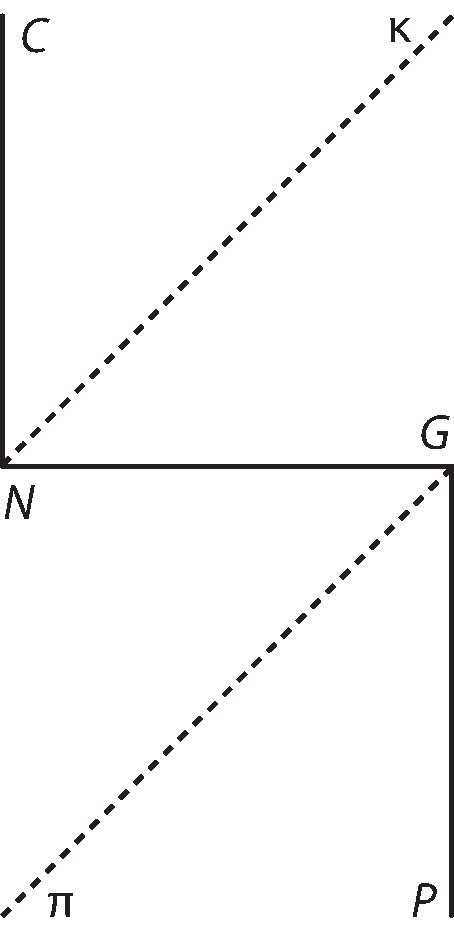
\includegraphics[trim = 0mm -3mm -5mm 0mm, clip, width=0.285\textwidth]{images/LH035,14,02_123v-d1.pdf}\\
\noindent
\centering
[\textit{Fig. 26}]\edtext{}{\lemma{\hspace*{1,8mm}[\textit{Fig. 26}]}\killnumber\Cfootnote{Vgl. \cite{00301}a.a.O., Fig. 336 (\cite{01008}\textit{WO} I, S. 1062).}}
\end{wrapfigure}
%%%%%%%%%
\edtext{%
Hinc inter Aristotelis\protect\index{Namensregister}{\textso{Aristoteles}, 384-322 v. Chr.}
\textit{quaestiones Mechanicas}[:] 
\textit{qui sedet, non potest se in rectam erigere
nisi protenso capite vel pedibus retractis.
%
Nempe qui sedet in situ $\displaystyle CNGP.$
factis angulis rectis in} punctis $\displaystyle N$ et $\displaystyle G.$
\textit{longe majorem corporis partem habet a $\displaystyle G$ versus $\displaystyle N$ positam,
(nempe totam partem $\displaystyle CNG$ a capite ad ge\-nua;)
adeoque centrum gravitatis,\protect\index{Sachverzeichnis}{centrum gravitatis}
ejusve perpendiculum procul a $\displaystyle G$ versus $\displaystyle N.$
Cum itaque stanti futurum sit fulcrum\protect\index{Sachverzeichnis}{fulcrum}
in pedibus\protect\index{Sachverzeichnis}{pes} $\displaystyle P$;
adeoque manentibus ut prius cruribus $\displaystyle GP$ in situ perpendiculari;
revocandum sit totius $\displaystyle CNG$ centrum ad perpendiculum $\displaystyle GP$
ut ipsi $\displaystyle G$ superemineat,
vix aut ne vix illud fiet,
nisi supra modum robustos supponamus musculos\protect\index{Sachverzeichnis}{musculus}
tendinesque\protect\index{Sachverzeichnis}{tendo} eo spectantes}[;]
\textit{erigendus est enim rotationis centro $\displaystyle G$ vectis\protect\index{Sachverzeichnis}{vectis}
$\displaystyle GN$ (et ipse gravis) onere\protect\index{Sachverzeichnis}{onus}
$\displaystyle NC$ in extremo onustus.
Si vero retrahantur pedes a $\displaystyle P$ ad $\displaystyle\pi$
% [...]
vel caput protendatur a $\displaystyle C$ ad $\displaystyle\kappa$ quo}
%Wallis, Mechanica, London 1670-1671, S. 769.
fulcrum centro gravitatis\protect\index{Sachverzeichnis}{centrum gravitatis} subjiciatur,
\textit{magno onere}
\edtext{levantur}{\lemma{levantur}\Cfootnote{In der Vorlage \textit{liberantur}.}}
\textit{musculi tendinesque.}}{%
\lemma{Hinc [...] \textit{tendinesque}}%
\Cfootnote{\cite{00301}a.a.O., S. 769 (\cite{01008}\textit{WO} I, S. 1062). Zitat mit Auslassungen.
Siehe \cite{01002}\textsc{Aristoteles}, \textit{Mech.} 30, 857b21-858a2.}} % Quaestiones mechanicae, Venedig 1585, S. 532.
%
\edtext{%
\textit{Hinc anser horrei ostium intrans utcunque altum
% [...]
caput\protect\index{Sachverzeichnis}{caput} demittit.}
% Wallis, Mechanica, London 1670-1671, S. 768.
Quod aliqui interpretantur ex simplicitate evitare velle capitis impactum,
sed vera ratio, quod limen\protect\index{Sachverzeichnis}{limen} superare conans,
\textit{pedum antecedente limini imposito
circa quod fulcrum\protect\index{Sachverzeichnis}{fulcrum} seu motus centrum}
% Wallis, Mechanica, London 1670-1671, S. 769.
rotanda totius corporis moles\protect\index{Sachverzeichnis}{moles}
seu \textit{centrum gravitatis}[,]
\textit{rotationem facilitat porrecto capite ultra limen,\protect\index{Sachverzeichnis}{limen}
adeoque aucta ipsius gravitatione\protect\index{Sachverzeichnis}{gravitatio} centrum totius}
[\textit{propius}]\edtext{}{\lemma{proprius}\Bfootnote{\textit{L ändert Hrsg. nach Vorlage}}}
% Wallis, Mechanica, London 1670-1671, S. 769.
\textit{fulcro\protect\index{Sachverzeichnis}{fulcrum} admovet.}
Idemque facimus, dum gradum, scalas\protect\index{Sachverzeichnis}{scala} montem ascendimus.}{%
\lemma{\textit{Hinc} [...] ascendimus}%
\Cfootnote{\cite{00301}J. \textsc{Wallis}, \textit{Mechanica}, pars III, cap. 15, London 1670-1671, S. 769f. (\cite{01008}\textit{WO} I, S. 1062). Zitate mit Auslassungen.}}
%
\pend
\pstart
\edtext{%
Ex eadem causa
\textit{Bajuli cum onus humeris seu tergo gestant
se antrorsum incurvant, si ulnis retrorsum,
et ancilla si aquae situlam promisso brachio sinistro ferat
dextrorsum se incurvat (}%
\edtext{exerto}{\lemma{exerto}\Cfootnote{In der Vorlage \textit{extento}.}}
\textit{etiam brachio\protect\index{Sachverzeichnis}{brachium} dextro)
si dextro sinistrorsum,
si utroque recta incedit,
similiterque si capiti impositam ferat.}
% Wallis, Mechanica, London 1670-1671, S. 770.
Vidi qui cum pondus\protect\index{Sachverzeichnis}{pondus} manibus jaceret,
\textit{cecidit ipse retrorsum.
Nempe quo corporis ponderisque commune centrum gravitatis
fulcro\protect\index{Sachverzeichnis}{fulcrum} immineret,
corporis centrum gravitatis\protect\index{Sachverzeichnis}{centrum gravitatis} nonnihil}
\edtext{loco}{\lemma{loco}\Cfootnote{In der Vorlage \textit{retro}.}}
\textit{motum erat, quod itaque ipsum,
post separatum quod manibus gestabat pondus,\protect\index{Sachverzeichnis}{pondus}
ita retraxit, ut antequam se in debitum situm}
\edtext{retrahere}{\lemma{retrahere}\Cfootnote{In der Vorlage \textit{restituere}.}}
\textit{posset, retro ceciderit.}}{%
\lemma{Ex eadem [...] \textit{ceciderit}}%
\Cfootnote{\cite{00301}a.a.O., S. 770 (\cite{01008}\textit{WO} I, S. 1062f.). Zitate mit Auslassungen.}}
% 
\pend
\pstart
Wallisius\protect\index{Namensregister}{\textso{Wallis} (Wallisius), John 1616-1703}
in suis notis id observat.
Non males ut literas adhibeat,
quae initialibus respondeant rei de qua agitur,
ut tempus\protect\index{Sachverzeichnis}{tempus} $\displaystyle t.$
pondus\protect\index{Sachverzeichnis}{pondus} $\displaystyle p.$
celeritas\protect\index{Sachverzeichnis}{celeritas} $\displaystyle c.$
vis,\protect\index{Sachverzeichnis}{vis} $\displaystyle v.$
impedimentum:\protect\index{Sachverzeichnis}{impedimentum} $\displaystyle i.$ etc. 
\pend
\vspace*{1em}
\pstart
% \noindent
\edtext{%
In capite V de calculo de centro gravitatis\protect\index{Sachverzeichnis}{centrum gravitatis} prop. 22.
notat Elementa curvae cycloeidis,\protect\index{Sachverzeichnis}{cycloeides}
axe\protect\index{Sachverzeichnis}{axis} in partes aequales innumeras diviso
esse ut secundanorum reciproca.}{%
\lemma{In capite [...] reciproca}%
\Cfootnote{\cite{00301}a.a.O., pars II, cap. 5, S. 429f. (\cite{01008}\textit{WO} I, S. 839).}}
%
[124~r\textsuperscript{o}] %%%%%%%%%%  HIER BEGINNT BLATT 124r. 
%
\pend
\pstart
\edtext{%
Primus observavit Wallisius,\protect\index{Namensregister}{\textso{Wallis} (Wallisius), John 1616-1703}
\textit{non} tantum \textit{semicycloeidem esse semicirculi triplam,
quod pridem innotuit,
sed et illius portiones hujus} portionibus \textit{respective esse triplas},
nempe $\displaystyle \beta b \tau\, \sqcap\, [3]\edtext{}{\lemma{3}\Bfootnote{\textit{erg. Hrsg. nach Vorlage}}} B \alpha B.$}{%
\lemma{Primus [...] $\displaystyle B \alpha B$}%
\Cfootnote{\cite{00301}a.a.O., S. 459 (\cite{01008}\textit{WO} I, S. 859). Zitat mit Auslassungen.}}
\pend
\pstart
\edtext{In libro hoc de motu,
Wallisius\protect\index{Namensregister}{\textso{Wallis} (Wallisius), John 1616-1703}
calculum ad omnes casus producit,
quod in libro de Cycloeide non fecerat,
principiis tantum exhibitis.}{\lemma{ In libro [...] exhibitis}%
\Cfootnote{\cite{00301}a.a.O., S. 458 (\cite{01008}\textit{WO} I, S. 858). Siehe J.\cite{00314} \textsc{Wallis}, \textit{Tractatus duo. Prior, de cycloide et corporibus inde genitis. Posterior ... de cissoide et corporibus inde genitis}, Oxford 1659, S. 1-74 (\cite{01008}\textit{WO} I, S. 499-541).}}
%
\edtext{%
Laloverae\protect\index{Namensregister}{\textso{Lalouv\`ere} (La Loubère, Lalovera), Antoine de 1600-1664}
calculus convenit \edtext{Wallisiano,
ex octo non nisi in duobus error.}{%
\lemma{Wallisiano,}\Bfootnote{%
\textit{(1)}\ exceptis in octo locis, error
\textit{(2)}\ exceptis
\textit{(3)}\ ex octo [...] error
\textit{L}}}}{%
\lemma{Laloverae [...] error}%
\Cfootnote{J.\cite{00301} \textsc{Wallis}, \textit{Mechanica}, pars II, cap. 5, London 1670-1671, S. 463-465 (\cite{01008}\textit{WO} I, S. 861f.). Siehe A.\cite{01057} \textsc{Lalouvère}, \textit{Veterum geometria promota in septem de cycloide libris}, Toulouse 1660.}}
\pend
%\newpage% PR: Rein provisorisch !!!
\vspace*{2.5em}
\pstart
\noindent\centering\setline{16}
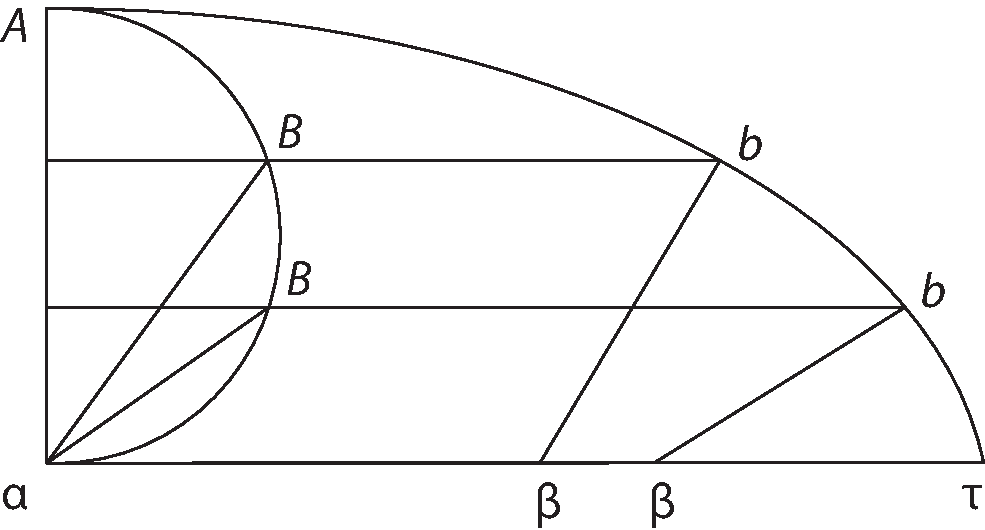
\includegraphics[width=0.58\textwidth]{images/LH035,14,02_124r-d1.pdf}\\%
\vspace*{0.2em}%
[\textit{Fig. 27}]\edtext{}{\lemma{\hspace*{1,8mm}[\textit{Fig. 27}]}\killnumber\Cfootnote{Vgl. \cite{00301}a.a.O., Fig. 166 (\cite{01008}\textit{WO} I, S. 802).}}
\pend
%\newpage
\count\Afootins=1200
\count\Bfootins=1000
\count\Cfootins=1000
\pstart
\edtext{%
Torricellii\protect\index{Namensregister}{\textso{Torricelli}, Evangelista 1608-1647}
\textit{Apologiam edidit Carolus Dati,}\protect\index{Namensregister}{\textso{Dati}, Carlo Roberto 1619-1676}
vel \textit{quisquis alius sub ficto nomine Timauri Antiatis,\protect\index{Namensregister}{\textso{Antiate}, Timauro \textit{siehe} Dati, Carlo Roberto} Florentiae 1663 lingua Italica.}}{%
\lemma{Torricellii [...] \textit{Italica}}%
\Cfootnote{J.\cite{00301} \textsc{Wallis}, \textit{Mechanica}, pars II, cap. 5, London 1670-1671, S. 462 (\cite{01008}\textit{WO} I, S. 860). Zitat mit Auslassungen. Siehe C.\cite{00032} \textsc{Dati}, \textit{Lettera a Filaleti di Timauro Antiate della vera storia della cicloide, e della famosissima esperienza dell'argento vivo}, Florenz 1663.}}
%
\pend
\pstart
\edtext{%
Collinius\protect\index{Namensregister}{\textso{Collins} (Collinius), John 1625-1683}
Wallisio\protect\index{Namensregister}{\textso{Wallis} (Wallisius), John 1616-1703}
1665 proposuerat \textit{tanquam rem maxime desideratam et quotidiani usus,
in mensurandis vasis vinariis partim depletis.}}{%
\lemma{Collinius [...] \textit{depletis}}%
\Cfootnote{J.\cite{00301} \textsc{Wallis}, \textit{Mechanica}, pars II, cap. 5, prop. 25, London 1670-1671, S. 477f. (\cite{01008}\textit{WO} I, S. 870). Wallis weist dort auf einen Brief von Collins mit Datum 12. August 1665 hin.}}
%
\edtext{%
Respondit Wallisius:\protect\index{Namensregister}{\textso{Wallis} (Wallisius), John 1616-1703}
\textit{redigendum esse expositum sphaeroeidos
vel dolii Truncati frustum, ad}
\edtext{inscriptum}{\lemma{inscriptum}\Cfootnote{In der Vorlage \textit{inscriptae}.}}
\textit{sphaerae frustum correspondens,
ad quod frustum
\edtext{illud sphaeroeidos eam}{%
\lemma{illud}\Bfootnote{%
\textit{(1)}\ sphaeroeidis eum
\textit{(2)}\ \textit{sphaeroeidos eam}
\textit{L}}}
habebit rationem,
quam habet sphaeroeidis axis ad diametrum sphaerae,
propter plana sphaeroeidis parallelis sphaerae
\edtext{planis correspondentibus aequalia,}{%
\lemma{planis}\Bfootnote{%
\textit{(1)}\ respondentia
\textit{(2)}\ \textit{correspondentibus aequalia}
\textit{L}}}
sed ab invicem ea ratione longius remota
quam habet Axis sphaeroeideos, ad axem sphaerae.
Illud autem sphaerae frustum,
considerandum esse tanquam ex pyramidibus conflatum,
communem verticem
\edtext{habentibus centrum}{%
\lemma{habentibus}\Bfootnote{%
\textit{(1)}\ in centro
\textit{(2)}\ \textit{centrum}
\textit{L}}}
sphaerae basesque in frusti superficie continuas}
\edtext{ipsum}{\lemma{ipsum}\Cfootnote{In der Vorlage \textit{ipsam}.}}
\textit{complentes.
Quorum quidem, quae bases planas habent, facile exhiberi posse;
cum plana illa}
\edtext{aliud}{\lemma{aliud}\Cfootnote{In der Vorlage \textit{alia}.}}
\textit{non sint quam circulorum portiones,
notis methodis exhibendae, earumque a centro distantiae
(altitudinem determinantes)
\edtext{facile exquirantur.}{%
\lemma{facile}\Bfootnote{%
\textit{(1)}\ exhibeantur
\textit{(2)}\ \textit{exquirantur}
\textit{L}}}
Quod autem ad eas innumeras}
[\textit{attinet}],\edtext{}{\lemma{continet}\Bfootnote{\textit{L ändert Hrsg. nach Vorlage}}}
\textit{quarum exiguae bases superficiem curvam complent,
cum basium aggregatum sit ea ipsa superficies curva,
et communis omnium altitudo,
radius sphaerae}[,]
\textit{id unum superesse posse difficultatis
ut exhibeatur illa superficies curva.
Id autem quicquid sit difficultatis
jam a se olim explicatum esse}
ait Wallisius\protect\index{Namensregister}{\textso{Wallis} (Wallisius), John 1616-1703}
\edtext{\textit{in subjunctis ad calcem tractatus de Cycloeide, pag. 122
(sed quae inferenda fuerant pag. 23. § 68)
ubi docetur figuram quamlibet in superficie sphaerae circulorum quorumvis
(sive maximorum, sive minimorum) arcubus terminatam quadrare.}}{%
\lemma{\textit{in subjunctis} [...] \textit{quadrare}}%
\Cfootnote{J.\cite{00314} \textsc{Wallis}, \textit{Tractatus duo}, Oxford 1659, S. 122 und S. 23 (\cite{01008}\textit{WO} I, S. 511).}}
\textit{Adeoque rem} illam non amplius inter desiderata censendam.}{%
\lemma{Respondit [...] censendam}%
\Cfootnote{\cite{00301}J.\cite{00301} \textsc{Wallis}, \textit{Mechanica}, pars II, cap. 5, London 1670-1671 S. 478 (\cite{01008}\textit{WO} I, S. 870f.).}}
%
\edtext{%
Haec Wallisius\protect\index{Namensregister}{\textso{Wallis} (Wallisius), John 1616-1703}
cap. V. prop. 26 fusius explicat.}{
\lemma{Haec [...] explicat}%
\Cfootnote{J.\cite{00301} \textsc{Wallis}, \textit{Mechanica}, pars II, cap. 5, London 1670-1671, S. 479-487 (\cite{01008}\textit{WO} I, S. 871-877).}}
%
\pend
\count\Afootins=1500
\count\Bfootins=1500
\count\Cfootins=1500
\pstart
\edtext{%
Wallis\protect\index{Namensregister}{\textso{Wallis} (Wallisius), John 1616-1703}
cap. V. prop. 28 monet \textit{in scholio} suae \textit{prop. 45 Arithm. infin.
in assignanda ratione quam habet figura spiralis ad sectorem conterminum
prout crescunt $\displaystyle MT$ radii in angulorum $\displaystyle AMT$
% [$\displaystyle PMT$]\edtext{}{\lemma{$\displaystyle AMT$}\Bfootnote{\textit{L ändert Hrsg. nach Vorlage}}}
ratione simpla, duplicata, \edtext{triplicata, quadruplicata}{\lemma{triplicata, quadruplicata}\Bfootnote{\textit{erg. L}}} etc.
Cum juxta demonstrationis tenorem
dicendum erat} esse \textit{ut 1 ad 3. 5. 7. 9 etc.
nescio qua incuria} irrepsit
\textit{ut 1 ad 3. 4. 5. 6 etc.
Quod cum non adverteret
Steph. ab Angelis,}\protect\index{Namensregister}{\textso{Angeli}, Stefano degli (Stephanus ab Angelis) 1623 - 1697}
prolixe refutatum ivit,
cum potuisset tribus verbis
\edtext{emendare, cum demonstratio}{%
\lemma{emendare, cum}\Bfootnote{%
\textit{(1)}\ in demostration
\textit{(2)}\ \textbar\ in \textit{streicht Hrsg.}\ \textbar\ demonstratio
\textit{L}}}
esset bona,
et ipse illo principio usus sit ad justum \textit{de spiralibus} volumen,
quod tamen adhuc longe angustius,
\edtext{quam unicum illud scholium.}{%
\lemma{quam}\Bfootnote{%
\textit{(1)}\ corollaria
\textit{(2)}\ unicum illud scholium
\textit{L}}}}{%
\lemma{Wallis [...] scholium}%
\Cfootnote{\cite{00301}a.a.O., S. 530 (\cite{01008}\textit{WO} I, S. 903f.). Siehe J.\cite{00315} \textsc{Wallis}, \textit{Arithmetica infinitorum}, Oxford 1656, S. 36f. (\cite{01008}\textit{WO} I, S. 385). S.\cite{01058} \textsc{degli Angeli}, \textit{De infinitorum spiralium spatiorum mensura}, Venedig 1660, S. 114-126.}}
%
\pend
%\newpage% PR: Rein provisorisch !!!!
\vspace*{2.0em}% PR: Rein provisorisch !!!!
%%%%%%%%%%%%%%%%%%%% PR: Bitte, Abbildungen korrekt setzen. Danke.
\pstart
% \vspace*{2em}
\noindent\setline{11}\centering
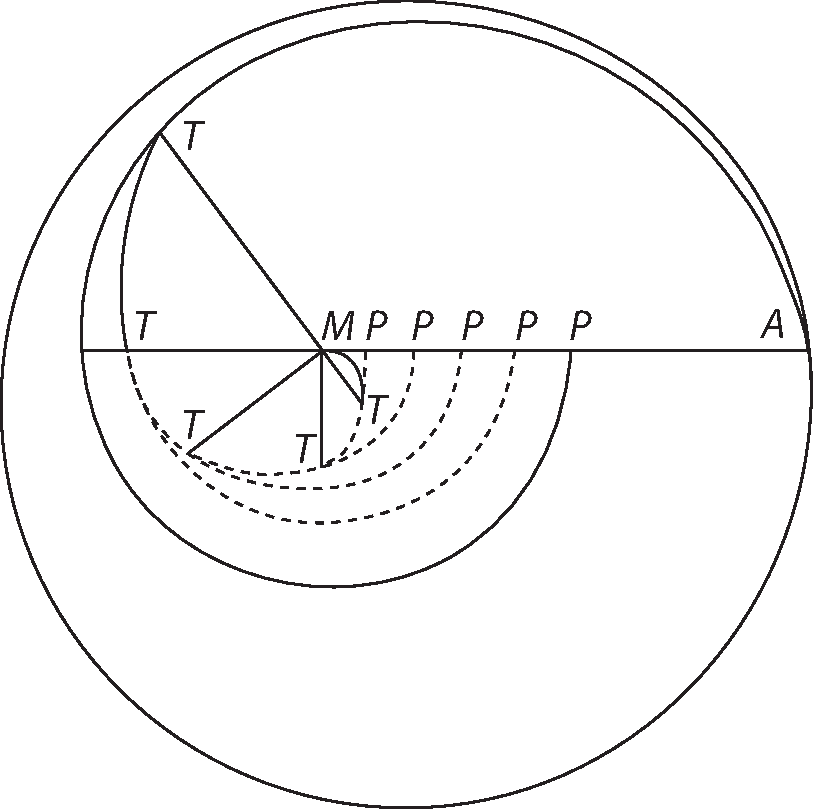
\includegraphics[width=0.56\textwidth]{images/LH035,14,02_124r-d2.pdf}\\%
%\vspace*{-0.3em}%
\rule[-4mm]{0mm}{10mm}[\textit{Fig. 28, erg. Hrsg. nach Wallis}]\edtext{}{\lemma{\hspace*{1,8mm}[\textit{Fig. 28}]}\killnumber\Cfootnote{Vgl. Abbildung in J.\cite{00315} \textsc{Wallis}, \textit{Arithmetica infinitorum}, Oxford 1656, S. 37 (\cite{01008}\textit{WO} I, S. 385).}}
\pend
\newpage
\count\Afootins=1100
\count\Bfootins=1100
\count\Cfootins=1100
\pstart
Cap. V. prop. 32.
% Wallis, Mechanica, London 1670-1671, S. 556.
\edtext{%
Habet Wallis\protect\index{Namensregister}{\textso{Wallis} (Wallisius), John 1616-1703}
inventum Wrenni\protect\index{Namensregister}{\textso{Wren} (Wrennus), Christopher 1632-1723}
\textit{qui solidum Hyperbolicum Convexo}[-]\textit{Concavum torni\protect\index{Sachverzeichnis}{tornus} ope,
acie dolabrae\protect\index{Sachverzeichnis}{dolabra} rectilinea obliquo ad axem situ posita conficere docuit.}}{%
\lemma{Habet [...] \textit{docuit}}%
\Cfootnote{J.\cite{00301} \textsc{Wallis}, \textit{Mechanica}, pars II, cap. 5, prop. 31, London 1670-1671, S. 555 (\cite{01008}\textit{WO} I, S. 930). Siehe C. \textsc{Wren}, \textit{Generatio corporis cylindroidis hyperbolici}, \textit{PT} 4 (1669), S.~961f.,\cite{01059} sowie \textit{A Descritption of C. Wren's Engin, designed for grinding Hyperbolical Glasses}, \textit{PT} 4 (1669), S. 1059f.\cite{01064}}}
%
Nimirum ita Wrennus,\protect\index{Namensregister}{\textso{Wren} (Wrennus), Christopher 1632-1723}
\edtext{%
\textit{si in quacunque ab axe torni distantia ponatur acies dolabrae recta,
in situ ad illum axem\protect\index{Sachverzeichnis}{axis}
(non parallelo, ut in tornando Cylindro, sed quocunque)
obliquo formabitur torno Cylindroeides Hyperbolicum convexo}[-]\textit{concavum.
% .
Et quidem ea Hyperbola,\protect\index{Sachverzeichnis}{hyperbola}
cujus semiaxis transversus aequatur minimae distantiae aciei dolabrae ab axe Cylindroeidis
(seu semidiametro basis inscripti Cylindri),
axisque conjugatus cum Asymptoto\protect\index{Sachverzeichnis}{asymptotos} eum}
\edtext{faciunt}{\lemma{faciunt}\Cfootnote{In der Vorlage (irrtümlich) \textit{faciat}.}}
\textit{angulum quem facit dolabrae acies recta cum recta axi torni parallela.
Unde patet methodus Cylindroeides torno formandi,
cujus sectio per axem data, sit data Hyperbola.
Solidi hujus sectiones plano factae}[,]
\textit{si planum illud sit ad axem solidi rectum}[,]
\textit{sunt Circuli.
Si ad axem minus obliquum quam est Asymptotos,}
\protect\index{Sachverzeichnis}{ellipsis}[\textit{Ellipses}].\edtext{}{\lemma{Ellipsis}\Bfootnote{\textit{L ändert Hrsg. nach Vorlage}}}
\textit{Si similiter inclinatum sit atque ipsa Asymptotos}[,]
\textit{sunt parabolae,\protect\index{Sachverzeichnis}{parabola}
vel si etiam per centrum sit, parallelogrammum.
Si adhuc obliquius secet axem, vel etiam sit axi parallelum,
oppositae Hyperbolae}[,]
\textit{vel si axi parallelum\protect\index{Sachverzeichnis}{axis}
atque per verticem hyperbolae genetricis}
\edtext{\lbrack%
\edtext{}{\lemma{\lbrack aut}\Cfootnote{Eckige Klammer von Leibniz.}}%
aut etiam si hyperbolam hanc ubivis tangat,
ut adscripsit \protect\index{Namensregister}{\textso{Huygens} (Hugenius, Ugenius, Hugens, Huguens), Christiaan 1629-1695}%
Hugenius\rbrack%
\edtext{}{\lemma{Hugenius\rbrack}\Cfootnote{Eckige Klammer von Leibniz.}}%
}{\lemma{aut etiam [...] Hugenius}\Cfootnote{Was Leibniz offenbar als Huygens' Bemerkung bewertet hat, ist eigent\-lich nur eine Ergänzung, die Huygens aus der Liste der \textit{Emendanda} am Ende des zweiten Bandes von Wallis' \textit{Mechanica} (nach S. 771) übernommen und an der gehörigen Textstelle im ersten Band eingefügt hatte.}}
\textit{opposita Triangula.}}{%
\lemma{\textit{si in} [...] \textit{Triangula}}%
\Cfootnote{J.\cite{00301} \textsc{Wallis}, \textit{Mechanica}, pars II, cap. 5, prop. 32, London 1670-1671, S. 556 (\cite{01008}\textit{WO} I, S. 930).}}
%
\pend
\pstart
\edtext{%
\textit{Intelligatur \edtext{fig. 215}{\lemma{fig. 215}\Cfootnote{Vgl. die Abbildung [\textit{Fig. 30}] auf S. \pageref{LH35,14,02_124r_ref-1}.}}
acies dolabrae\protect\index{Sachverzeichnis}{dolabra} recta}
[$\displaystyle AOO$],\edtext{}{\lemma{$\displaystyle AOO$}\Bfootnote{\textit{erg. Hrsg. nach Vorlage}}}
\textit{in quacunque ab axe\protect\index{Sachverzeichnis}{axis} cylindroeidis
torno\protect\index{Sachverzeichnis}{tornus} conficiendi distantia situ quocunque obliquo (ad axem illum) posita.
Manifestum est per rectam illam $\displaystyle AOO$ transiturum esse planum aliquod ut $\displaystyle OA\alpha$
cui parallelus sit cylindroeidis axis $\displaystyle C\delta .$
Rectamque aliquam in eo plano axi parallelam,
ut $\displaystyle A\alpha\alpha$
(nempe ex parallelis eam quae sit axi proxima)
lineam contactus} illam \textit{esse,
qua planum illud tangat cylindrum
(cylindroeidi inscriptum)
cujus \edtext{axis $\displaystyle C\delta,$}{%
\lemma{axis}\Bfootnote{%
\textit{(1)}\ $\displaystyle OD$
\textit{(2)}\ $\displaystyle C\delta$
\textit{ L}}}
et basis radius $\displaystyle CA$
(quae est minima distantia aciei dolabrae\protect\index{Sachverzeichnis}{dolabra}
quantum opus sit}
%
[124~v\textsuperscript{o}] %%%%%%%%%%  HIER BEGINNT BLATT 124v.
%
\textit{continuatae ab axe cylindri seu cylindroeidis formandi)
sumtisque in axe
$\displaystyle C\delta\delta$ partibus continue aequalibus $\displaystyle C\delta,$ $\displaystyle \delta\delta,$ etc.
atque ad eum perpendicularibus $\displaystyle CA,$ $\displaystyle \delta\alpha,$ etc.
erectisque itidem ad planum $\displaystyle CA\alpha$ perpendicularibus, $\displaystyle \alpha O,$ $\displaystyle \alpha O,$ etc.
manifestum est rectas $\displaystyle \alpha O$ esse ut 1. 2. 3 etc.}
% [...]
et [earum]\edtext{}{\lemma{eorum}\Bfootnote{\textit{L ändert Hrsg. nach Vorlage}}}
\textit{quadrata, ut horum quadrata, et propterea
(propter angulum $\displaystyle \delta\alpha O$ rectum rectasque $\displaystyle \alpha\delta$ invicem aequales)
junctis omnibus $\displaystyle O\delta$ quadrata harum esse,
ut quadrata numerorum illa aequalibus quadratis aucta.\\
%%
\hspace*{7,5mm}%
Adeoque si torni ope circa axem $\displaystyle C\delta$ (fig. 215) describi intelligantur
in Cylindroeide Circuli quorum radii sint ipsae $\displaystyle \delta O$ rectae,
sectio per axem exhibebit ipsum $\displaystyle \delta CAO$
\edtext{figurae 214}{\lemma{figurae 214}\Cfootnote{Vgl. die Abbildung [\textit{Fig. 29}] auf S. \pageref{LH35,14,02_124v_ref-1}.}} planum.
Erunt utique circulorum illorum radii planum complentes ipsis $\displaystyle \delta O$ utriusvis figurae aequales.
Nempe si in binis figuris, sumtis tum $\displaystyle AC$ aequalibus,
tum aequalibus $\displaystyle C\delta$ respectivis, sumantur $\displaystyle \alpha O$
fig. 215 ipsis $\displaystyle C\delta$ fig. 214 respectivis aequales.
Quod fit sumto $\displaystyle OA\alpha$
\edtext{fig. 215 angulo semirecto}{%
\lemma{fig. 215}\Bfootnote{%
\textit{(1)}\ \textit{}ipsis $\displaystyle C\delta$ fig. 214 respectivis aequales
\textit{(2)}\ \textit{angulo semirecto}
\textit{L}}}
(qualis est in fig. 214. $\displaystyle \delta CM$
quem cum axe conjugato $\displaystyle C\delta$ facit Asymptotos $\displaystyle CM.$}%
[\textit{)}]\edtext{}{\lemma{\textit{)}}\Bfootnote{\textit{erg. Hrsg. nach Vorlage}}}
\textit{Si vero alius sit angulus $\displaystyle OA\alpha$ quam semirectus,
illi congruet Hyperbolae quae similem habeat angulum $\displaystyle \delta CM.$
ut nempe $\displaystyle C\delta$ fig. 214. 215. sint respectivis $\displaystyle \alpha O$ fig. 215 aequales.\\
%%
\hspace*{7,5mm}%
Constat itaque non modo cylindroeides hujusmodi torno formari posse,
cujus sectio per axem sit Hyperbola,
sed et quae sit data Hyperbola.
Quippe exponatur Hyperbola AOO fig. 214 quaelibet,
cujus centrum $\displaystyle C.$ semiaxis transversus $\displaystyle CA.$ axis
\edtext{conjugatus $\displaystyle C\delta.$}{%
\lemma{conjugatus}\Bfootnote{%
\textit{(1)}\ $\displaystyle CD.$
\textit{(2)}\ $\displaystyle C\delta.$
\textit{L}}}
et Asymptota $\displaystyle CM.$
cui similem imperatum sit torno exhibere.
Hoc tantum curandum erit,
nempe ut $\displaystyle CA$ fig. 215 sit aequalis ipsi $\displaystyle CA$
fig.} [\textit{214}]\edtext{}{\lemma{215}\Bfootnote{\textit{L ändert Hrsg. nach Vorlage}}}
\textit{sitque angulus $\displaystyle \alpha AO$ fig. 215 ipsi $\displaystyle \delta CM$ fig. 214
quem cum Asymptoto facit axis conjugatus, aequalis.}\\
%%
\hspace*{7,5mm}%
Hoc idem solidum fit
\textit{conversione Hyperbolae
\edtext{$\displaystyle AOO$}{\lemma{$\displaystyle AOO$}\Cfootnote{In der Vorlage $\displaystyle OAO.$}}
fig.}\edtext{ \edtext{214}{\lemma{214}\Cfootnote{In der Vorlage \textit{216}. Wallis bezieht sich hierbei auf eine weitere Abbildung, die Leibniz nicht berücksichtigt.}}%
}{\lemma{\textit{fig.}}\Bfootnote{
\textit{(1)}\ \textit{216}
\textit{(2)}\ 214
\textit{L}}}
\textit{circa axem}
\edtext{\textit{conjugatum} $\displaystyle C\delta.$%
\edtext{}{\lemma{$\displaystyle C\delta$}\Cfootnote{In der Vorlage $\displaystyle \delta C\delta.$}}}{%
\lemma{\textit{conjugatum}}\Bfootnote{%
\textit{(1)}\ $\displaystyle CD.$
\textit{(2)}\ $\displaystyle C\delta.$
\textit{L}}}}{%
\lemma{\textit{Intelligatur} [...] \textit{conjugatum} $\displaystyle C\delta$}%
\Cfootnote{J.\cite{00301} \textsc{Wallis}, \textit{Mechanica}, pars II, cap. 5, London 1670-1671, S. 558f. (\cite{01008}\textit{WO} I, S. 931f.). Zitat mit Auslassungen.}}
%
\pend
\pstart
Egregium hoc sane est
Wrenni\protect\index{Namensregister}{\textso{Wren} (Wrennus), Christopher 1632-1723} inventum,
et videndum \edtext{an quid simile pro Ellipsi et parabola}{%
\lemma{an}\Bfootnote{%
\textit{(1)}\ Circulus, Ellipsis et para
\textit{(2)}\ Sphaera,
\textit{(3)}\ \textit{}quid [...] parabola
\textit{L}}}
comminisci liceat, utendo
\edtext{scilicet acie non}{%
\lemma{scilicet}\Bfootnote{%
\textit{(1)}\ non
\textit{(2)}\ acie non
\textit{L}}}
rectilinea sed circulari.
Ita enim fiet figurae obliqua aciei circularis
\edtext{positione tornatae constructio}{%
\lemma{positione}\Bfootnote{%
\textit{(1)}\ descriptae
\textit{(2)}\ tornatae
\textit{(a)}\ descriptio
\textit{(b)}\ constructio
\textit{L}}}
non difficilior, quam quae est sphaerae.  
\pend
\newpage% PR: Rein provisorisch !!!
\pstart
\begin{minipage}[t]{0.50\textwidth}
\hspace*{-10mm}
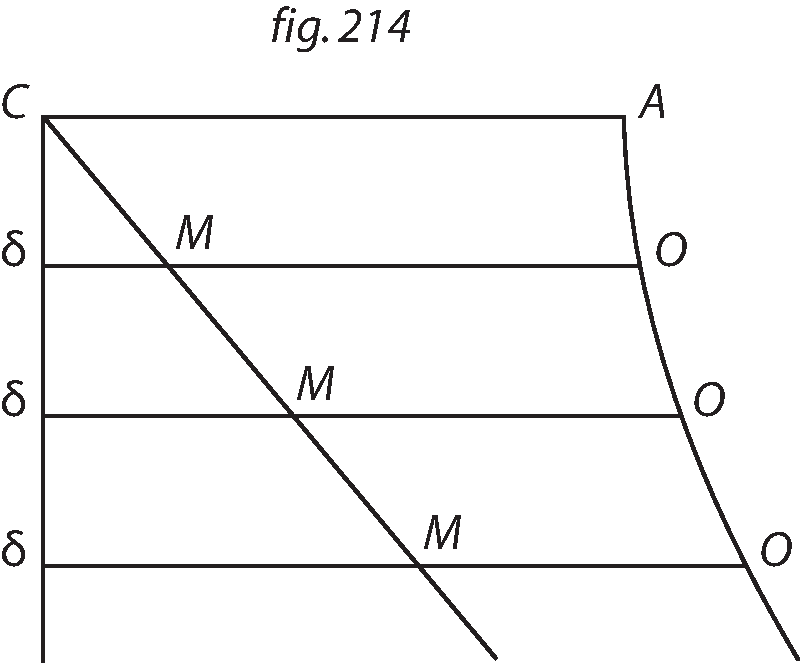
\includegraphics[width=0.9\textwidth]{images/LH035,14,02_124v-d1.pdf}\\
\\
\noindent\centering\hspace*{-10mm}[\textit{Fig. 29}]\label{LH35,14,02_124v_ref-1}
\end{minipage}
\hspace*{-5mm}
\begin{minipage}[t]{0.50\textwidth}
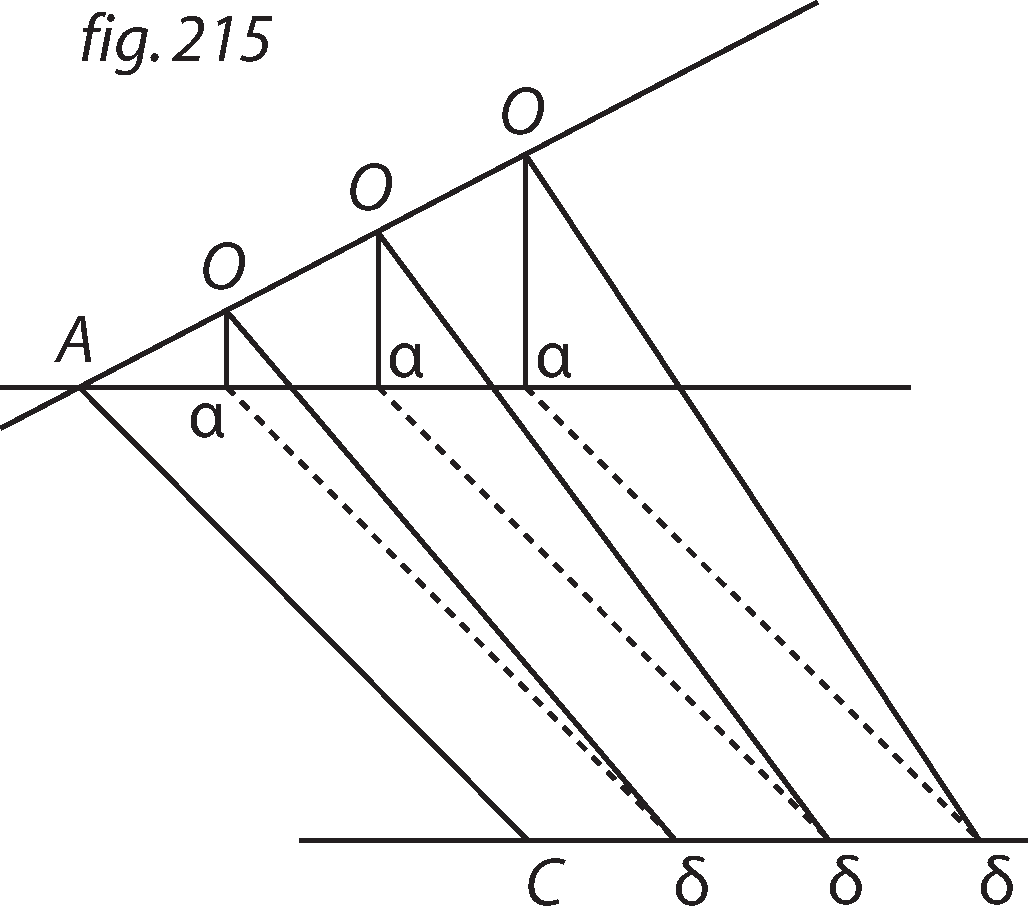
\includegraphics[width=0.83\textwidth]{images/LH035,14,02_124v-d2.pdf}\\
\\
\noindent\centering%\hspace*{-10mm}
[\textit{Fig. 30}]\label{LH35,14,02_124r_ref-1}
% \vspace{1em}% PR: Rein provisorisch !!!
\end{minipage}
\edtext{}{\lemma{\hspace*{1,8mm}[\textit{Fig. 29}]}\killnumber\Cfootnote{Vgl. \cite{00301}a.a.O., Fig. 214 (die Abbildung fehlt in \cite{01008}\textit{WO} I).}}%
\edtext{}{\lemma{\hspace*{1,8mm}[\textit{Fig. 30}]}\killnumber\Cfootnote{Vgl. \cite{00301}a.a.O., Fig. 215 (\cite{01008}\textit{WO} I, S. 931).}}%
\pend
\count\Afootins=1500
\count\Bfootins=1500
\count\Cfootins=1500
%%%%
%%%% ENDE von Bl. 124v und vom ganzen Stück.